\chapter{Analyse du rehaussement}
\label{sec:Analysis}
Nous avons présenté dans les chapitres précédents les problématiques liées aux images médicales (Chap. 1), puis nous avons illustré les grandes familles de rehaussement de vaisseaux (Chap. 2). Nous avons ensuite construit un banc de test capable d'évaluer l'influence du rehaussement sur des zones d'intérêt précises (Chap. 3). Enfin, nous avons traité un ensemble de bases de données publiques de manière à définir 6 zones d'intérêt spécifiques dont nous rappelons brièvement les notations :

\begin{itemize}
\item Un masque global de l'organe \maskglobal.
\item Un masque de voisinage (union des zones internes et externes adjacentes des vaisseaux)  \maskvascular.
\item Des masques de voisinage des vaisseaux basés sur la taille : \maskvesselLarge, \maskvesselMedium, \maskvesselSmall.
\item Un masque des bifurcations \maskbif.
\end{itemize}

\section{Conditions initiales}

Dans ce chapitre, nous mettons à profit l'ensemble des connaissances et outils vus précédemment afin d'analyser en détail sept filtres de rehaussement de vaisseaux. Pour commencer, nous récapitulons rapidement les bases de données utilisées ainsi que les filtres sélectionnés avant de définir les métriques et la méthode d'évaluation utilisée.

\subsection{Base de données}
Nous avons à disposition trois bases de données présentées dans le Chap. 2 : l'Ircad, une base de 20 volumes en tomodensitométrie ; trois versions de VascuSynth, contenant chacune 120 volumes, définies avec différents niveaux de bruit ricien $\sigma=\{2,4,6\}$ et Bullitt, une base de 33 volumes IRM en phase T2, auquel on a ajouté du bruit ricien ($\sigma=4$) et des biais en intensités. Nous disposons, pour ces jeux de données, des vérités terrains binaires des vaisseaux ainsi que des masques construits précédemment et rappelés en début de chapitre.

Le choix de cette évaluation par zones permet d'enrichir significativement l'analyse, par rapport à une analyse globale classique. En effet, le rehaussement global et le rehaussement vasculaire local peuvent être de qualités très différentes. C'est par exemple le cas de filtres sensibles aux structures en plateaux telles que les bordures des organes. L'évaluation par taille apporte, elle aussi, une information supplémentaire sur les limites du rehaussement à l'échelle macro et microscopique. Elle permet de plus de quantifier quelle partie du réseau vasculaire rehaussé participe le plus aux performances globales. Enfin, la répartition en zones permet d'évaluer les performances des filtres sur des parties peu représentatives de l'ensemble du réseau vasculaire, mais qui peuvent être critiques dans certaines applications. C'est par exemple le cas des bifurcations pour le suivi de lignes centrales.

Les sept filtres choisis pour cette analyse sont ceux détaillés dans le Chap. 2 et dont la construction cherche à répondre à des problématiques spécifiques différentes. Ces particularités sont résumées dans la table \ref{tab:diffMethods}. 

\begin{table}[ht]
  \begin{center}
    \resizebox{\textwidth}{!}{
\begin{tabular}{l|l|l|l}
Méthode                               & Base                  &  Idée principale                              &   Date  \\ \hline  \hline 
Sato et al.      & Hessienne               & Reconnexion des vaisseaux et contrôle du bruit  & 1997   \\ \hline
Frangi et al.    & Hessienne             & Contrôle du bruit ainsi que des structures en plateaux et sphériques   & 1998   \\ \hline
Meijering et al. & Hessienne             & Détection de structures fines                          & 2004 \\ \hline
OOF et al.       & Flux               & Contraindre de l'analyse à la surface d'une sphère pour limiter le débordement de la réponse               & 2010 \\ \hline
Jerman et al.    & Hessienne             & Augmenter l'homogénéité de la réponse et simplifier la paramétrisation            & 2016 \\ \hline
Zhang et al.     & Hessienne              & Limiter le rehaussement des bordures du foie         & 2018 \\ \hline
RORPO et al.     & Morphologie            & Discriminer les structures tubulaires par un vote de chemins orientés                         & 2018  
\end{tabular}
    }
\end{center}
\caption{Liste des filtres disponibles dans le banc de test ainsi que leur principale caractéristique.}
\label{tab:diffMethods}
\end{table}

\section{Métriques}

Pour cette expérience, nous utilisons plusieurs métriques. La majorité des métriques utilisées repose sur la comparaison voxel à voxel entre le résultat binarisé d'un filtre et un jeu de paramètres donné.

On peut classifier les voxels selon 4 classes différentes : Les vrais positifs ($VP$) lorsqu'il y a une correspondance 1-1 entre le $i^{ème}$ voxel du résultat binaire et le $i^{ème}$ voxel de la vérité terrain, les vrais négatifs ($VN$) pour une correspondance 0-0, les faux positifs ($FP$) lors d'une correspondance 1-0 et les faux négatifs ($FN$) pour une correspondance 1-0. Ces quatres classes quelques fois représentés sous la forme d'une matrice de confusion (Tab. \ref{tab:confusion_matrix}).

\begin{table}
  \centering
  \begin{tabular}{ cccc }
    \hline
                                      &   &\multicolumn{2}{c}{Vérité terrain} \\
                                      &   & 0  & 1 \\
      \multirow{2}{*}{prédiction}     & 0 & VN & FN \\
                                      & 1 & FP & VP  \\
    \hline
  \end{tabular}
  \caption{Matrice de confusion. $VN$ : Vrais négatifs, $FP$ : faux positifs, $FN$ : faux négatifs, $VP$ : Vrais positifs}
  \label{tab:confusion_matrix}
\end{table}

Un certain nombre de métriques issues de ces quantités sont utilisées de manière classique dans la littérature. Ces métriques sont définies entre $0$ et $1$, avec $1$ le meilleur score possible. 

\paragraph{Précision}
La précision représente la proportion de voxels prédits positifs par rapport à la proportion de voxels positifs prédits totaux.
\begin{equation}
  Précision = \frac{VP}{VP+FP}
\end{equation}

Cette mesure permet d'évaluer la proportion de voxels correctement classifiés par rapport aux voxels prédits positifs.

\paragraph{Sensibilité}

La sensibilité est la proportion de voxels positifs prédits parmi les positifs réels.

\begin{equation}
  Sensibilité = \frac{VP}{P} = \frac{VP}{VP+FN}
\end{equation}

Cette mesure permet d'évaluer si le filtre est capable de détecter tous les vaisseaux annotés par la vérité terrain et dans quelle proportion certains vaisseaux ne sont pas détectés. 

\paragraph{Spécificité}

La spécificité est la proportion de voxels négatifs correctement prédits parmi les voxels négatifs réels.

\begin{equation}
  Spécificité = \frac{VN}{N} = \frac{VN}{VN+FP}
\end{equation}

Cette mesure permet d'évaluer si le filtre rehausse des structures non annotées dans la vérité terrain. Elle est l'équivalent pour les vrais négatifs de la sensibilité.

\paragraph{Justesse}

La justesse, est une métrique plus large que la précision. Elle prend en compte le classement correct des voxels positifs et négatifs. 

\begin{equation}
  Justesse = \frac{VP+VN}{P+N} = \frac{VP+VN}{VP+VN+FP+FN}
\end{equation}

La précision mesure la qualité de la classification globale, à la fois le bon rehaussement et à la fois l'absence de faux rehaussement.

Bien que toutes ces mesures soient informatives d'un aspect particulier de la segmentation, elles n'ont pas toutes le même poids. En effet, les vaisseaux représentent moins de 5 \percent{}de l'ensemble des voxels d'un volume. Le poids des voxels négatifs peut donc dans une certaine mesure être très supérieur au poids des voxels positifs. On peut ainsi être amené avec la justesse à sous-estimer des erreurs de segmentation. Les mesures les plus significatives pour nos expériences parmi ces mesures, sont la sensibilité et la précision.


\paragraph{Dice}

Le score de Dice, aussi connu sous le nom de F1-score est une mesure de recouvrement entre le volume binaire de la vérité terrain et le volume binaire prédit. Il s'exprime comme l'intersection sur l'union de la vérité terrain et du volume binaire prédit.

\begin{equation}
  \textrm{Dice} = \frac{2 \textrm{VP}}{\textrm{FP} + \textrm{FN} + 2 \textrm{VP}} \\ 
\end{equation}

Le Dice est une mesure populaire dans la littérature, mais il n'exprime que le recouvrement des voxels positifs correctement classifiés. Un recouvrement total aura une mesure de $1$ là où un recouvrement nul aura une mesure de $0$. Cette mesure est performante lorsque l'on s'intéresse à maximiser l'intersection entre la vérité terrain et la segmentation. Cependant, elle ne permet pas de différencier un ensemble de segmentations qui auraient un nombre similaire de vrais positifs, mais dont la proportion de FP et de FN est différente. Pour notre analyse, il est en effet souhaitable d'avoir une métrique qui permet de différencier les sur-segmentations et les sous-segmentations. Dans notre analyse, le Dice sert donc de mesure d'évaluation secondaire. Il permet notamment d'évaluer les performances du rehaussement des bifurcations, puisque la métrique principale n'est pas défini dans cette zone d'intérêt.

\paragraph{Coefficients de corrélation de Matthew}

Les coefficients de corrélation de Matthew (MCC), un cas spécifique du score $\phi$ \cite{Chicco2020_advantages_MCC_Dice}, est plus  expressif que le Dice puisqu'il intègre la classification correcte du fond, les vrais négatifs, dans la mesure. Cette métrique est définie entre $-1$ et $1$ avec $1$ un volume binaire égal à la vérité terrain et $-1$ un volume binaire étant le complémentaire de la vérité terrain.

\begin{equation}
  \textrm{MCC} = \frac{TP \cdot TN - FP \cdot FN}{\sqrt{(TP+FP)(TP+FN)(TN+FP)(TN+FN)}}
\end{equation}

Bien que le Dice est plus commun dans la littérature, le MCC est présenté par Chicco et Jurman \cite{Chicco2020_advantages_MCC_Dice} comme une mesure plus stable pour les structures éparses telles que les vaisseaux. Le MCC n'est pas défini dans un certain nombre de cas, et notamment lorsque les zones d'intérêt sur lesquelles sont caculées les métriques ne contiennent pas de voxels négatifs. Pour ces zones, on utilise le Dice pour l'évaluation. 


\paragraph{Rapport signal sur bruit}

%\todo{ Est-ce que je garde le SNR sachant qu'au final on ne l'a jamais exploité ?}

Nous avons souhaité intégrer une mesure au banc de test qui ne dépende pas d'un processus de binarisation mais qui exprime la distance entre la vérité terrain et la sortie du filtre. Nous avons choisi le PSNR, qui est habituellement utilisé pour évaluer le degré de dégradation d'une image causée par du bruit. On illustre habituellement ce processus par le cas d'un message qui subirait des pertes lorsque que celui-ci est envoyé à travers un canal de communication. On peut assimiler le  Le PSNR est défini par :

\begin{align}%\label{Eq: SNR_and_PSNR}
  %\nonumber
  %\textrm{SNR} & = \log_{10}\Big( \frac{1}{|I|}\frac{ \sum_{x} I_{\textrm{Filter}}(x)^2 }{ \sum_{x} I_{\textrm{Ground-truth}}(x)^2 } \Big) \\
 \nonumber
  \textrm{PSNR} & = \log_{10}\Big( \frac{ (\max_x I(x))^2  }{ \textrm{MSE}( I_{\textrm{GT}}, I_{\textrm{Filtre}} ) } \Big)
\end{align}

Avec $I$ l'image de sortie normalisée, $I_{filtre}$ l'image filtrée, $I_{GT}$ l'image binaire normalisée et MSE l'erreur au sens des moindres carrés. Plus le PSNR est haut, plus l'image filtrée est proche de l'image binarisée. Dans le cas où les deux sont égales, le PSNR est infini.

Dans notre cas, nous utilisons le PSNR comme une mesure de similarité entre la sortie du filtre non binarisée et la vérité terrain normalisée (0 ou 1). Afin que des comparaisons fiables puissent être effectuées entre deux sorties de filtres, il est nécessaire de faire une mise à l'échelle de l'intensité de sortie du filtre entre 0 et 1 et de la vérité terrain (1 et non 255). En effet, nous nous sommes assuré que tous les filtres aient une sortie définie entre 0 et 1 (Chap. 3) mais rien ne garantit que la plage de rehaussement couvre l'ensemble de l'intervalle [0,1] et non un intervalle quelconque comme [0,0.3]. Il n'y a en effet pas de raisons, autre que pour des considérations de visualisation par l'œil humain, de différencier deux filtres (ou jeux de paramètres) produisant le même résultat binaire après seuillage, mais dont la dynamique est définie sur deux plages différentes.

Un faible PSNR nous indique soit que le rehaussement est très bruité, soit qu'il déborde ou alors que le niveau général de l'intensité du rehaussement est faible.


\paragraph{Courbe ROC}

La courbe ROC (\textit{Receiving Operator Caracteristic}) est une visualisation de l'évolution du taux de vrai positif en fonction du taux de faux positif au fur et à mesure des seuillages successifs appliqués au filtre. Pour rappel, Le taux de vrai positif correspond à la sensibilité et le taux de faux positif est égal à $1-\text{spécificité}$. 

Cette courbe donne une vue globale différente sur les performances des filtres pour différents seuils. Elle nous permet d'évaluer asymptotiquement les performances entre deux filtres alors que les autres métriques nous servent à quantifier les performances optimales d'un filtre. 

Lors de la construction de courbes ROC, il convient d'éviter une erreur lors du calcul. Une courbe ROC classique est définie par un ensemble de points $P$ qui forment généralement un pseudo arc de cercle entre les points (0,0) et (1,1). Dans le cas des filtres de rehaussement, la répartition des points sur l'arc est très hétérogène. Cette hétérogénéité dépend souvent de la diversité géométrique des structures rehaussées, car deux structures qui possèdent la même géométrie ont une valeur de rehaussement similaire. Au contraire, des structures différentes seront détectées à des seuils de tubularité différents. Ce point devient problématique lorsque l'on veut calculer une courbe ROC moyenne pour un filtre et un jeu de paramètres donnés appliqués à l'ensemble des volumes d'une base. Par exemple, si l'on possède trois courbes ROC de 200 points chacune représentée sous la forme d'une liste de points, on ne peut pas moyenner les points en fonction des indices ( $m_i = (ROC^1_{i} + ROC^2_{i} + ROC^3_{i})/3 $). Les points ne sont en effet pas échantillonnés de la même manière sur la courbe et la moyenne est faussée (Fig. \ref{fig:good_and_bad_roc}). Pour résoudre ce problème, il est nécessaire d'interpoler chaque courbe de manière à obtenir le même échantillonnage régulier sur chaque courbe. On obtient ainsi une courbe moyenne réellement représentative de la moyenne des ROC.

\begin{figure}[ht]
  \centering
  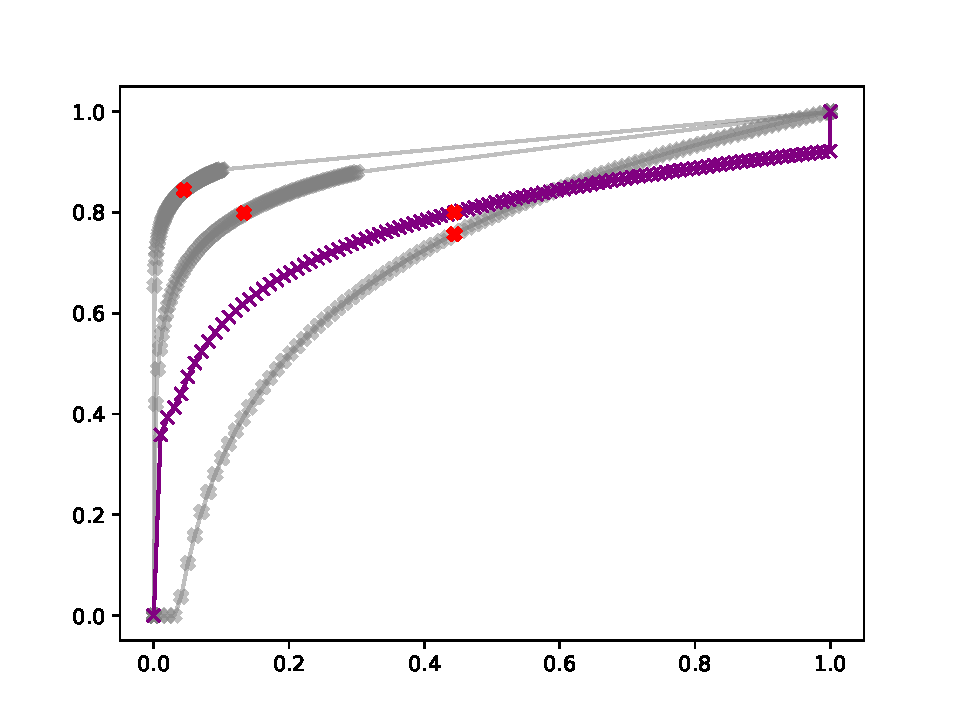
\includegraphics[height=5cm]{Images/ROC_badMean.pdf}
  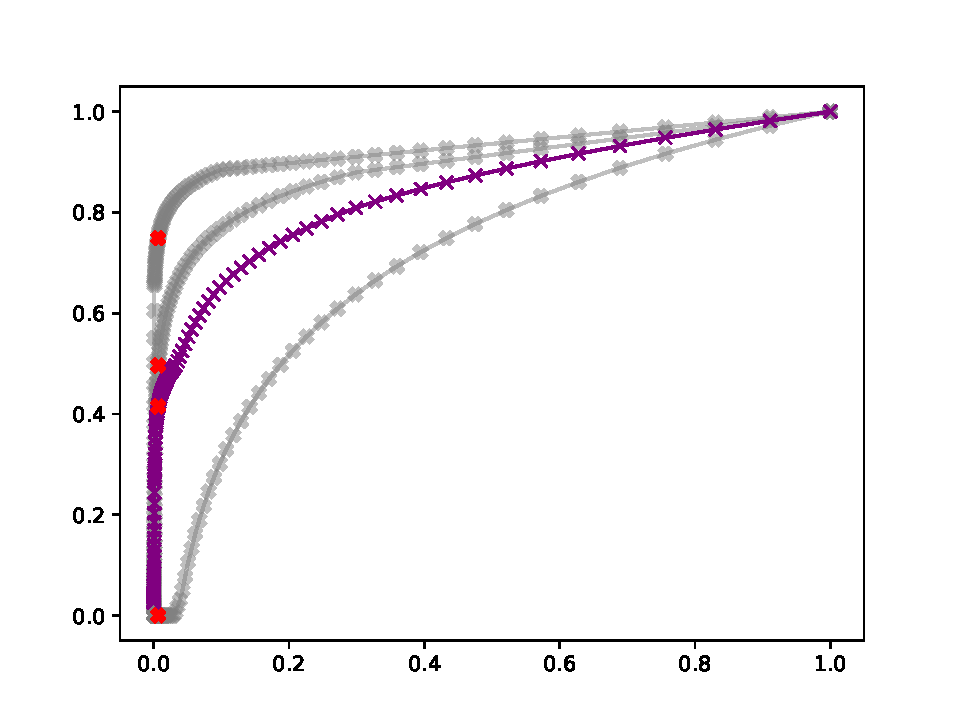
\includegraphics[height=5cm]{Images/ROC_goodMean.pdf}
  \caption{En violet courbe ROC moyenne construite à partir des courbes ROC en gris. À gauche, la courbe moyenne est construite sans interpolation. À droite, courbe ROC avec interpolation.}
  \label{fig:good_and_bad_roc}
\end{figure}

\section{Optimisation}

Nous avons cherché à comprendre si une paramétrisation optimale des filtres était nécessaire et s'il existait des règles pratiques régissant le choix des paramètres. En effet, les paramètres sont décrits par des considérations géométriques théorique, mais la manière de les régler est rarement décrite. À la place, des paramètres par défaut sont proposés. C'est par exemple le cas de Frangi ($\alpha=0.5,\beta=0.5$), ou Sato $(\alpha_1=0.5,\alpha_2=2$) dont les recommandations sont reprises dans de nombreux articles. Ces paramètres sont rarement discutés. Pourtant, dans certains articles plus applicatifs, les paramètres utilisés par les auteurs sont différents. Par exemple, Marcan et al. \cite{Marcan2014_vessel_seg} pour la segmentation dans l'IRM du foie proposent d'utiliser ($\alpha=0.3,\beta=0.7$) dans leur chaîne de segmentation. On peut donc légitimement se demander quel est l'impact des paramètres sur le rehaussement final et quels paramètres utiliser en fonction d'une base de données spécifique.

Pour répondre à cette question, nous avons cherché à optimiser les filtres de manière à proposer un rehaussement optimal pour une segmentation la plus élémentaire possible. Ainsi, l'objectif est de pouvoir analyser le rehaussement au plus près des filtres sans prétraitements ou des post-traitements qui pourraient cacher des spécificités des filtres. Par exemple, un traitement qui consiste à conserver les composantes connexes supérieurs à 100 voxels minimiserait l'analyse de la robustesse des filtres au bruit.

Nous avons choisi de définir l'optimalité du rehaussement par rapport au MCC mesuré entre la vérité terrain binaire des vaisseaux et les volumes filtrés puis binarisés. Le MCC permet non seulement de mesurer la qualité du rehaussement des vaisseaux, mais aussi de hiérarchiser plus précisément le rehaussement de structures erronées, contrairement au Dice. L'optimalité d'une métrique dépend aussi de la zone d'intérêt sélectionnée pour effectuer l'optimisation. Pour cela, nous avons choisi le masque \maskglobal afin de prendre en compte l'ensemble des problématiques du rehaussement : la détection des vaisseaux, la  différenciation avec les autres structures, la qualité du filtrage et l'amélioration du signal des vaisseaux. Nous aurions également pu choisir de maximiser le rehaussement des vaisseaux en utilisant leur voisinage comme zone d'optimisation. On aurait ainsi trouvé les paramètres donnant un rehaussement optimal des vaisseaux. Cependant, pour des considérations de temps, de puissance de calcul et de volume de données à analyser, nous avons choisi de n'optimiser les paramètres que par rapport à une seule zone d'intérêt.

L'ensemble des paramètres liés aux filtres de rehaussement peuvent être classifiés en deux groupes : les paramètres d'échelle qui définissent la fenêtre permettant de capturer la taille des vaisseaux et les paramètres intrinsèques des méthodes permettant de détecter la forme des vaisseaux. Par exemple, le filtre de Frangi possède 3 paramètres liés à l'échelle et trois paramètres qui pondèrent le filtrage en fonction de la géométrie. Quand un nombre élevé de paramètres (i.e $K \gg 1$) nécessite d'être optimisé (e.g. $k=6$ pour Frangi), trouver un jeu de paramètres optimal induit par l'espace à $k$-dimensions est coûteux en temps de calcul.

Dans nos expériences, nous avons choisi d'optimiser l'ensemble des paramètres en deux étapes :

\begin{itemize}
\item L'optimisation de l'échelle en utilisant des paramètres intrinsèques fixes.
\item L'optimisation des paramètres intrinsèques en utilisant le jeu d'échelles optimales trouvé à l'étape précédente.
\end{itemize}

Les paramètres intrinsèques fixes sont ceux recommandés par les auteurs des méthodes ou sont choisis empiriquement.  Pour chaque étape, les paramètres optimaux sont définis au sens du meilleur MCC moyen dans le masque global (\maskglobal) du jeu de données entier. Cette stratégie en deux étapes peut être comparée à un choix naturel où un utilisateur commence dans un premier temps par choisir les paramètres d'échelles en se basant sur des observations des structures biologiques avant de raffiner le rehaussement (Fig. \ref{fig:flowchart_opti}).

\begin{figure}[!ht]
  \centering
  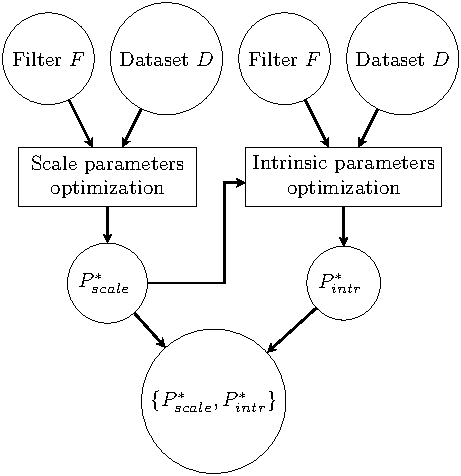
\includegraphics[height=6cm]{Images/flowchart_benchmark.pdf}
  \caption{Diagramme illustrant l'optimisation en deux temps. D'abords l'optimisation de l'échelle puis l'optimisation des paramètres intrinsèques.}
  \label{fig:flowchart_opti}
\end{figure}


\subsection{Méthode de calcul}
\subsubsection{calcul du MCC moyen}

  Notre définition du MCC moyen a connu deux formulations successives afin de supprimer les biais présents dans la première définition (Fig. \ref{fig:illustration_opti}). 
  
  Nous présentons la méthode de calcul du MCC moyen pour un  seul filtre et une seule base de donnée. En réalité nous avons calculé le MCC moyen de tous les jeux de paramètres pour tous les filtres sur l'ensemble des bases de données. De plus, le MCC moyen optimal est calculé pour la zone d'intérêt \maskglobal, mais une fois le jeu de paramètre optimal trouvé, la moyenne de chacune des métriques présentées précédement est calculée pour ce jeu de paramères dans les six zones dintérêts. Le calcul de la moyenne de chaque métrique est effectué de la même manière que celle du MCC.

  \begin{figure}[H]
    \centering
    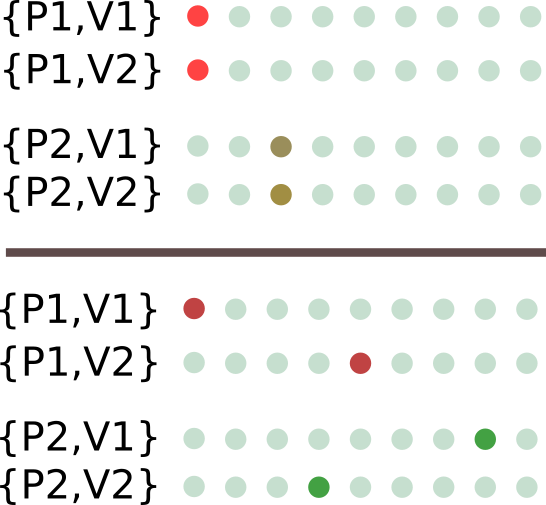
\includegraphics[height=6cm]{Images/optim.png}
    \caption{Illustration des deux itérations pour le calcul du MCC moyen. Exemple pour deux volumes $V1$ et $V1$ filtrés par les jeux de paramètres $P1$ et$P2$ En haut, l'itération $1$ reposant sur la moyenne des MCC des seuils de volumes filtrés. En bas, l'itération 2 reposant sur la moyenne des seuils maximisant le MCC.}
    \label{fig:illustration_opti}
  \end{figure}    

  \paragraph{Première itération}

  Soit $F$ un filtre de rehaussement et $D$ un jeu de données. Soit $P$ l'ensemble des jeux de paramètres. 
  $\forall p \in P$, $\forall v \in D$ :
  \begin{equation}
    R_{p,v} = F_{p}(v)
  \end{equation}
  Soit l'ensemble $S$ des seuillages appliqués à $R$ tel que $\forall s \in S$ :
  \begin{equation}
    RS_{p,v,s} = seuillage(R_{p,v}) 
  \end{equation}
  Soit la valeur du MCC $MCC_{p_i,v_j,s_k}$ calculé pour le volume seuillé $RS_{p_i,v_j,s_k}$.
  Alors le MCC moyen par seuil $\overline{MCC}_{p_i,s_k}$ est défini par :
  \begin{equation}
    \overline{MCC}_{p_i,s_k} = \frac{1}{N}\sum_{j=0}^{N} MCC_{p_i,v_j,s_k}
  \end{equation}
  Le meilleur MCC moyen $\overline{MCC}_{p_i}$ par jeu de paramètres est défini par : 
  \begin{equation}
    \overline{MCC}_{p_i} = \arg\max_{\forall s_k \in S} \overline{MCC}_{p_i,s_k}
  \end{equation}
  Le meilleur jeu de paramètres $p*$ est défini comme le jeu de paramètre dont le MCC moyen est maximal.
  \begin{equation}
    p* = \arg\max_{p_i \in P} \overline{MCC}_{p_i}
  \end{equation}

  Cette méthode, utilisée dans nos premiers travaux \cite{Lamy2020_VPH_bench}\cite{Lamy2021_RRPR}\cite{Lamy2020_ICPR}\cite{Lamy2021_ORASIS}, souffre des mêmes limitations qu'une moyenne effectuée naïvement pour calculer des courbes ROC. Elle moyenne en effet des rehaussements ayant des dynamiques différentes, ce qui sous-estime les résultats. La démarche initiale de cette méthode était d'émuler un fonctionnement où un opérateur aurait à manipuler un algorithme de segmentation paramétré une seule fois pour une utilisation régulière.
  
  \paragraph{Deuxième itération}
  Pour la deuxième itération, il a été choisi de maximiser le MCC du rehaussement dès l'étape de seuillage en choisissant le seuil maximisant le MCC par volume, plutôt que de moyenner le MCC par seuil sur l'ensemble des volumes. 

  Soit $F$ un filtre de rehaussement et $D$ un jeu de données. Soit $P$ l'ensemble des jeux de paramètres. 
  $\forall p \in P$, $\forall v \in D$ :
  \begin{equation}
    R_{p,v} = F_{p}(v)
  \end{equation}
  Soit l'ensemble $S$ des seuillages appliqués à $R$. tel que $\forall s \in S$ 
  \begin{equation}
    RS_{p,v,s} = seuillage(R_{p,v}) 
  \end{equation}
  Soit la valeur du MCC $MCC_{p_i,v_j,s_k}$ calculé pour le volume seuillé $RS_{p_i,v_j,s_k}$.
  Alors le MCC maximal par volume $MCC_{p_i,v_j}^{max}$ est défini par :
  \begin{equation}
    MCC_{p_i,v_j}^{max} = \max_{\forall s_k \in S} MCC_{p_i,v_j,s_k}
  \end{equation}
  Le meilleur MCC moyen $\overline{MCC}_{p_i}$ par jeu de paramètres est défini par : 
  \begin{equation}
    \overline{MCC}_{p_i} = \frac{1}{N} \sum_{j=0}^{N} MCC_{p_i,v_j}^{max}
  \end{equation}
  Le meilleur jeu de paramère $p*$ est défini comme le jeu de paramètre dont le MCC moyen est maximal.
  \begin{equation}
    p* = \arg\max_{p_i \in P} \overline{MCC}_{p_i}
  \end{equation}

  Dans cette itération, on émule un fonctionnement où un opérateur est capable de paramétrer pour chaque volume le seuil idéal. On tire donc le maximum des performances du pipeline de segmentation. Cette manière de procéder est utilisée aux deux étapes de l'optimisation sans changement de l'algorithme. Dans notre analyse du rehaussement, le pas appliqué entre chaque seuil est de 0.005, ce qui conduit à 201 seuils binaires. Cette méthode est utilisé dans nos travaux \cite{Lamy2022_TMI}.

  \subsubsection{Choix des paramètres}

Une stratégie de recherche exhaustive (\textit{grid search}) est réalisée pour ces paramètres. Les conditions de cette recherche sont résumés dans les tables \ref{tab:SS_interval}, \ref{tab:SS_interval_RORPO} (paramètres d'échelles) et tables \ref{table:PS_interval} (paramètres intrinsèques).

Le choix des paramètres a été fait de manière à trouver un compromis entre temps de calcul total du banc de test, espacement des paramètres et exhaustivité. Les limites des paramètres d'échelles ont été définies à la main en mesurant la taille des structures des troncs des réseaux vasculaires pour la limite haute et les limites de la résolution d'un pixel pour la limite basse. Une échelle inférieure à un pixel n'aurait en effet pas de sens pour les espaces gaussiens et de flux. La mesure de la taille des structures a été effectuée sur des images isotropes de résolution $[1\textrm{mm},1\textrm{mm},1\textrm{mm}$. 

Nous avons aussi intégré des limites de distances entre deux échelles successives d'un même jeu de paramètres. Cette limite permet d'éviter les jeux de paramètres aux échelles redondantes. C'est poruquoi, tout jeu de paramètres d'échelle dont la différence entre chaque échelle successive est inférieure à $\frac{1}{6}mm$ est éliminé. Pour RORPO, la taille minimale et maximale des chemins a été choisie empiriquement par validation visuelle. Une limite minimale à la tailles entre deux chemins successifs pour un jeu de paramètre a aussi été déterminé empiriquement de manière à limiter la redondance.
 %Un jeu de paramètres de RORPO est composé d'une taille de chemin minimale $e_{min}$, d'un facteur d'échelle $f$ et d'un nombre d'itérations $i$ qui permettent de définir une suite géométrique $e_i = e_{min} \times f^i$. 

 \begin{table}[H]
  \caption{Paramètres d'échelles pour les filtres utilisant un espace d'échelles basé sur le diamètre :  Frangi, Sato, Meijering, Jerman, Zhang, OOF. Les conditions  assurent que l'écart entre chaque échelle $i$ est supérieur à la résolution d'un voxel.}
  \label{tab:SS_interval}
  \begin{center}
    \begin{tabular}{  l  c  c  c }
      \hline
      \multicolumn{4}{c}{ Ircad et VascuSynth }\\
      \hline
      Paramètres & Intervalle & Pas & Conditions \\
      \hline
      $\sigma_{\min}$ & $[0.4,1.8]$ & $0.4$ & \\
      $\sigma_{\max}$ & $[1.4,3.4]$  & $0.4$ & $\sigma_{min,i} - \sigma_{max,i} > \frac{1}{6}$ mm \\ 
      Nombre d'échelles & $[\![3,4]\!]$ & $1$ & \\
      \hline
      \hline
      \multicolumn{4}{c}{ Bullitt }\\
      \hline
      Paramètres & Intervalle & Pas & Conditions \\
      \hline
      $\sigma_{\min}$ & $[0.2,1.6]$ & $0.4$ & \\
      $\sigma_{\max}$ & $[1.2,3.2]$  & $0.4$ & $\sigma_{min,i} - \sigma_{max,i} > \frac{1}{6}$ mm \\ 
      Nombre d'échelles & $[\![3,4]\!]$ & $1$ & \\
      \hline
    \end{tabular}
  \end{center}
\end{table}

\begin{table}[H]
  \caption{ Paramètres d'échelles pour RORPO sans le paramètre de dilatation. Les conditions d'espacement entre chaque échelle $i$ assure que deux échelles successives ne soient pas similaires.}
  \label{tab:SS_interval_RORPO}
  \begin{center}
    \begin{tabular}{  l  c  c  c }
      \hline
      \multicolumn{4}{c}{Ircad}\\
      \hline
      Paramètres & Intervalle & Pas & Conditions \\
      \hline
      Échelle min. & $[30,150]$ & $10$ & \\
      Facteur & $[1.1,1.6]$ & $0.1$ & $20 < \textrm{échelle}_{i} - \textrm{échelle}_{j} < 200$ \\ 
      Nb. d'échelles & $[\![2,4]\!]$ & $1$ & \\
      \hline
      \hline
      \multicolumn{4}{c}{Bullitt}\\
      \hline
      Paramètres & Intervalle & Pas & Conditions \\
      \hline
      Échelle min. & $[30,90]$ & $10$ & \\
      
      Facteurs & $[1.1,1.5]$  & $0.1$ & $ 20 < \textrm{échelle}_{i} - \textrm{échelle}_{j} < 200$ \\
      Nb. échelles & $[\![2,4]\!]$ & $1$ & \\
      \hline
      \hline
      \multicolumn{4}{c}{VascuSynth}\\
      \hline
      Paramètres & Intervalle & Pas & Conditions \\
      \hline
      Échelle min. & $[10,90]$ & $10$ & \\
      
      Facteur & $[1.1,1.5]$  &  $0.1$ & $ 9 < \textrm{échelle}_{i} - \textrm{échelle}_{j} < 100$ \\
      
      Nb. d'échelles & $[\![2,4]\!]$ & $1$ & \\
      \hline
    \end{tabular}
  \end{center}
\end{table}

\begin{table}[H]
  \caption{Paramètres intrinsèques : Meijering et RORPO n'ont pas de paramètre intrinsèque.}
  \label{table:PS_interval}
  \begin{center}
    \begin{tabular}{  l  c  c  c }
      \hline
      Filtres & Paramètres & Intervalle & Pas \\
      \hline
      Frangi & $\alpha$ & $[0.2,1.0]$ & $0.2$ \\
      ---       & $\beta$ & $[0.2,1.0]$ & $0.2$  \\
      ---       & $C$& $[0,60]$ & $30$ \\
      Sato & $\alpha_{1}$ & $[0.2,1.0]$ & $0.2$ \\
      ---     & $\alpha_{2}$ & $[1,2]$ & $0.2$ \\
      OOF & $\sigma$ & $[0.1,1.0]$ & $0.1$ \\
      Jerman & $\tau$ & $[0.1,1.0]$ & $0.1$ \\
      Zhang & $\tau$& $[0.1,1.0]$ & $0.1$ \\
      \hline
    \end{tabular}
  \end{center}
\end{table}
  
Au total, 41 jeux de paramètres d'échelle sont testés pour les filtres hessiens et OOF. Respectivement 32, 44 et 51 jeux de paramètres sont testé pour RORPO sur l'Ircad, VascuSynth et Bullitt. Pour les paramètres intrinsèques, 10 jeux de paramètres sont testés pour Jerman, Zhang et OOF. 75 jeux de paramètres sont testés pour Frangi et 30 pour Sato.


\section{Résultats}

Dans cette section, nous présentons et discutons les résultats quantitatifs et qualitatifs des différents filtres. En plus des sept filtres présentés précédemment, nous ajoutons un simple seuillage comme référence. La sortie de cette référence est l'image d'entrée normalisée et seuillée de manière à ce le seuil soit optimisé de la même manière que les autres paramètres.

Dans la suite, nous commençons par analyser les résultats des filtres dans le masque global \maskglobal. Puis, nous discutons des résultats obtenus sur les masques vasculaires \maskvascular, \maskvesselLarge, \maskvesselMedium, \maskvesselSmall. Enfin, nous exposons les résultats obtenus au niveau des bifurcations.

\subsection{Résultats globaux}

\todo{Je ne parle jamais des courbes ROC. Je ne sais pas où les introduires. Idem s'il faut les commenter, car les remarques sur les autres métriques couvrent déjà la plupart des points visibles sur les ROC. Il ne me semble pas que l'on commente les courbes dans le TMI non plus...}

\begin{figure}[!ht]
  \centering
  \begin{subfigure}[t]{\textwidth}
    \centering
    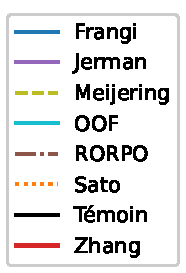
\includegraphics[clip = true, height=8cm]{Images/standAloneLegend.pdf}
  \end{subfigure}
\end{figure}
\begin{figure}[!ht]
  \begin{subfigure}[t]{\textwidth}
    \centering
  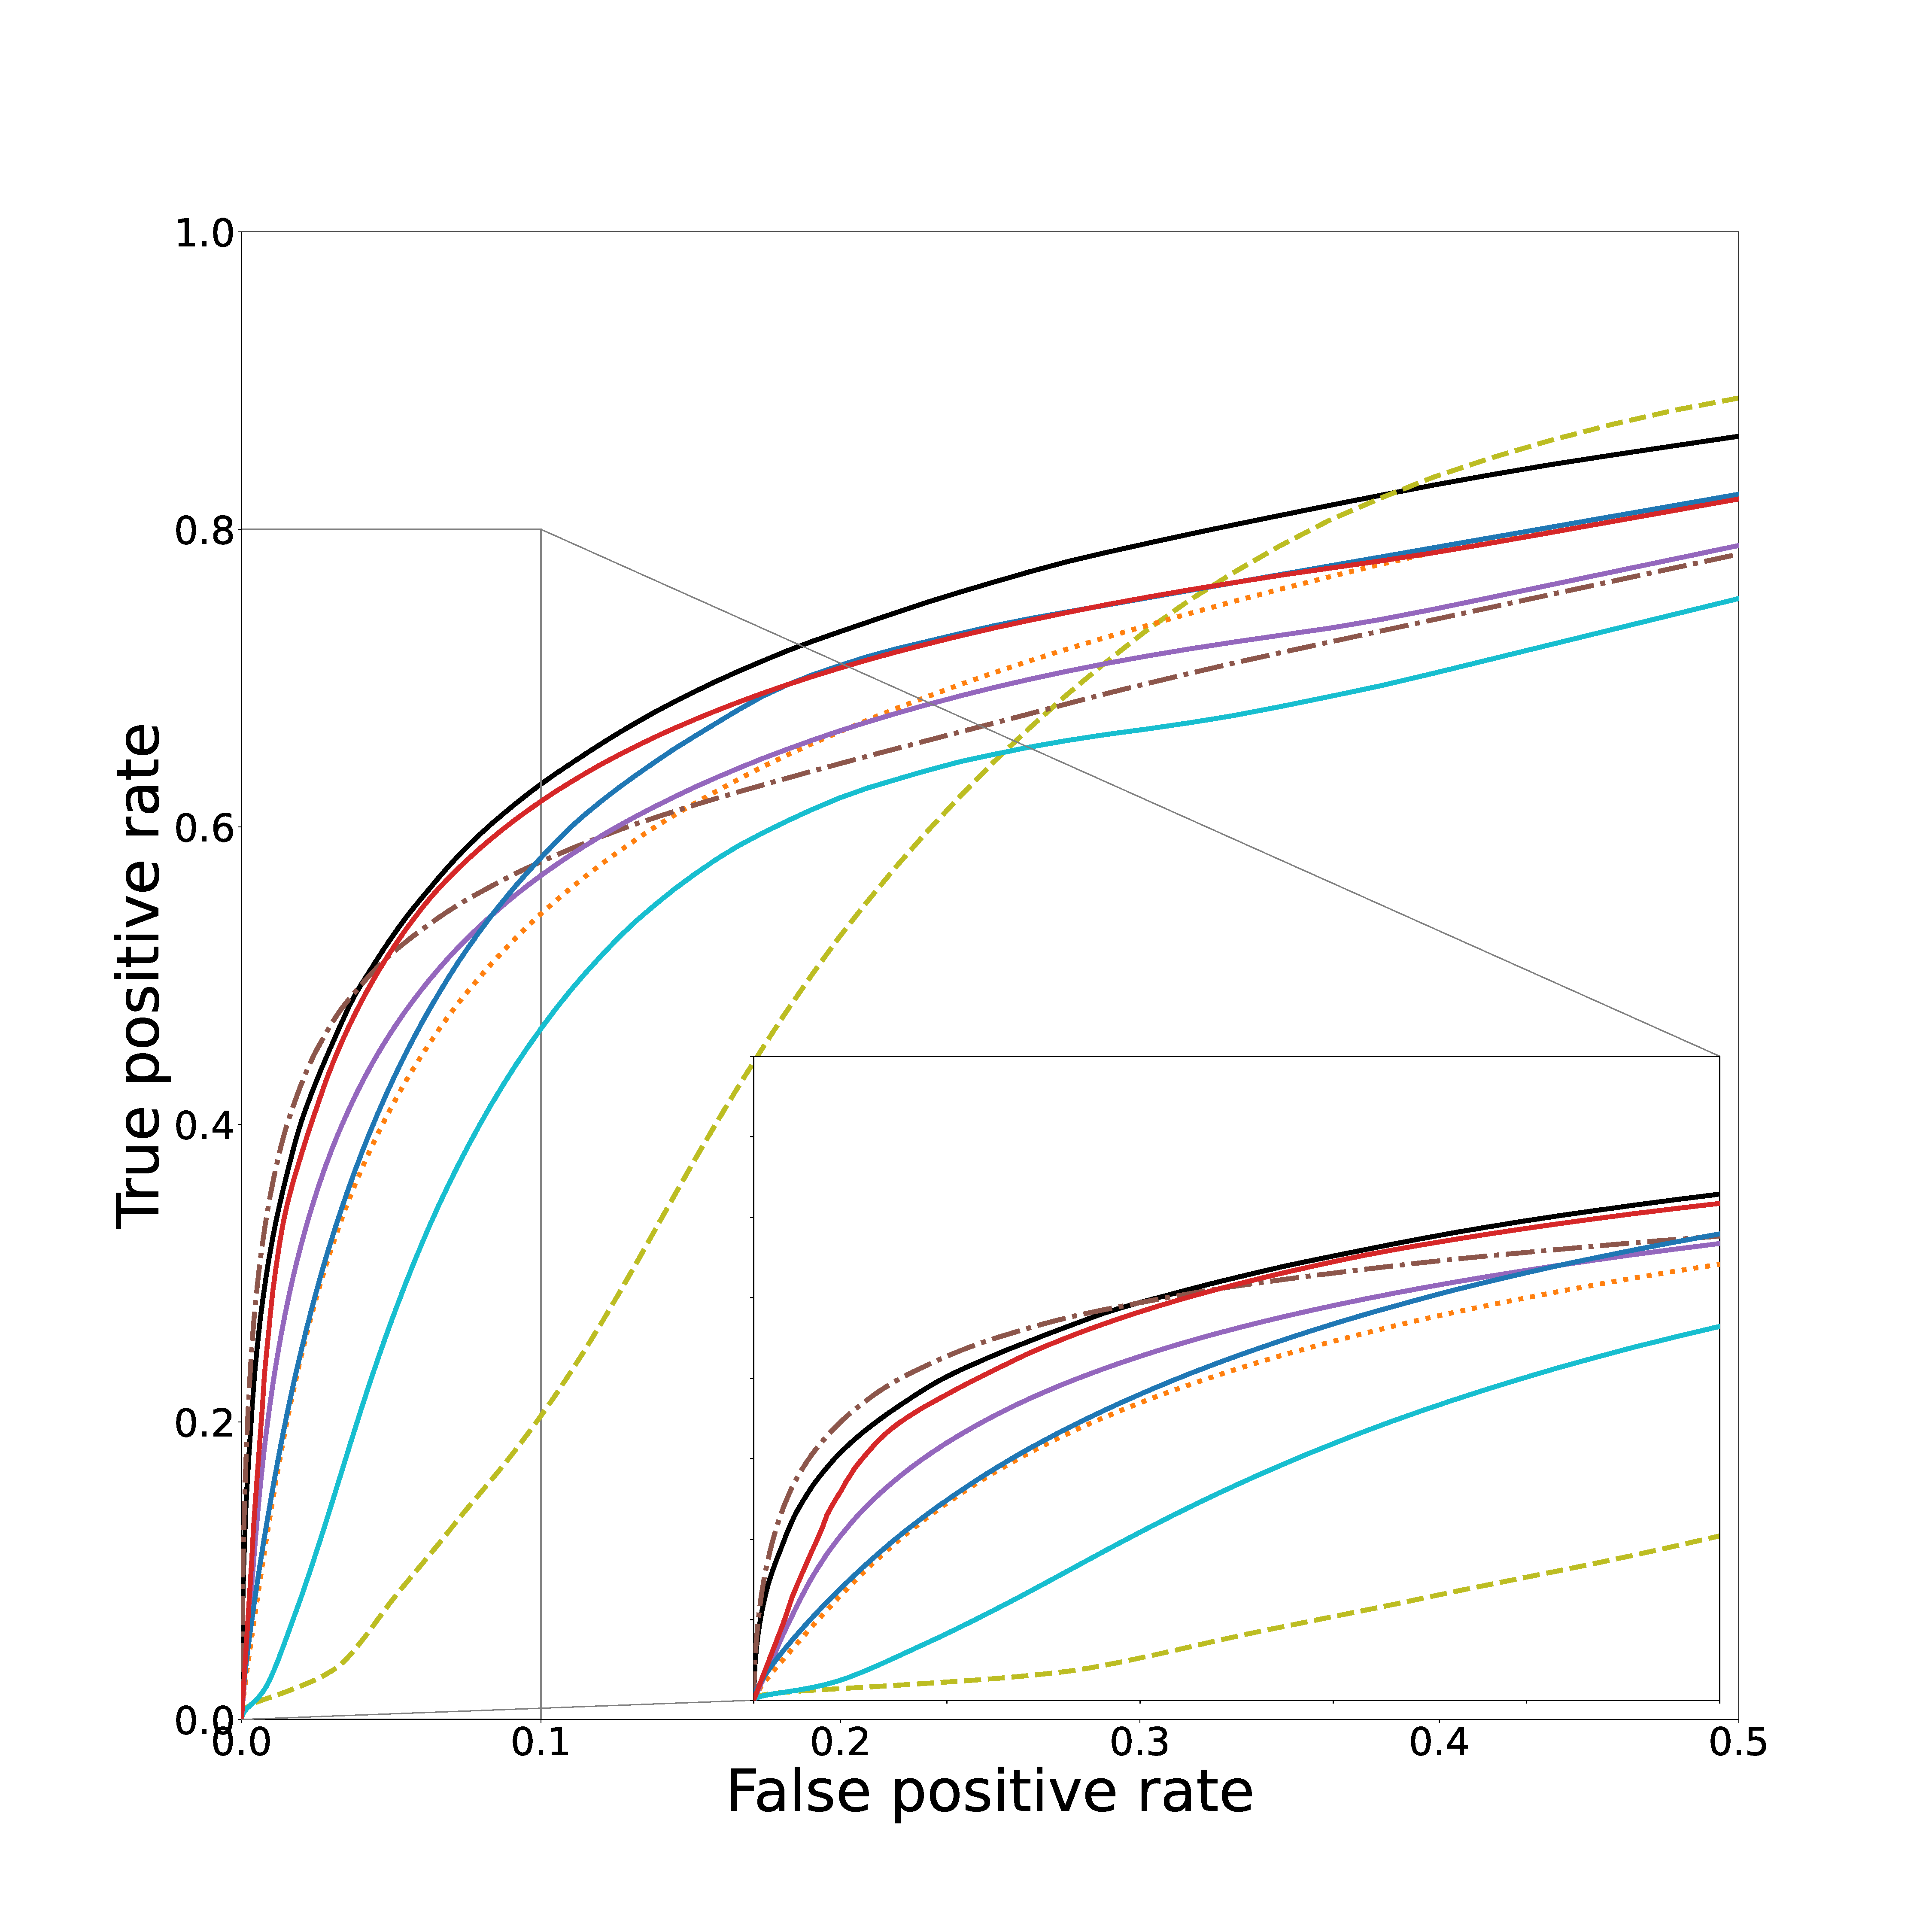
\includegraphics[clip = true, trim  =  125 125 180 260, height=9cm]{Images/Ircad_ROC.pdf}
  \caption{Ircad}
  \end{subfigure}
  \caption{Courbe ROC moyenne des sept filtres de rehaussement pour le jeu de l'Ircad}
  \label{fig:Ircad_ROC}
\end{figure}

\begin{figure}[!ht]
  \begin{subfigure}[t]{\textwidth}
    \centering
  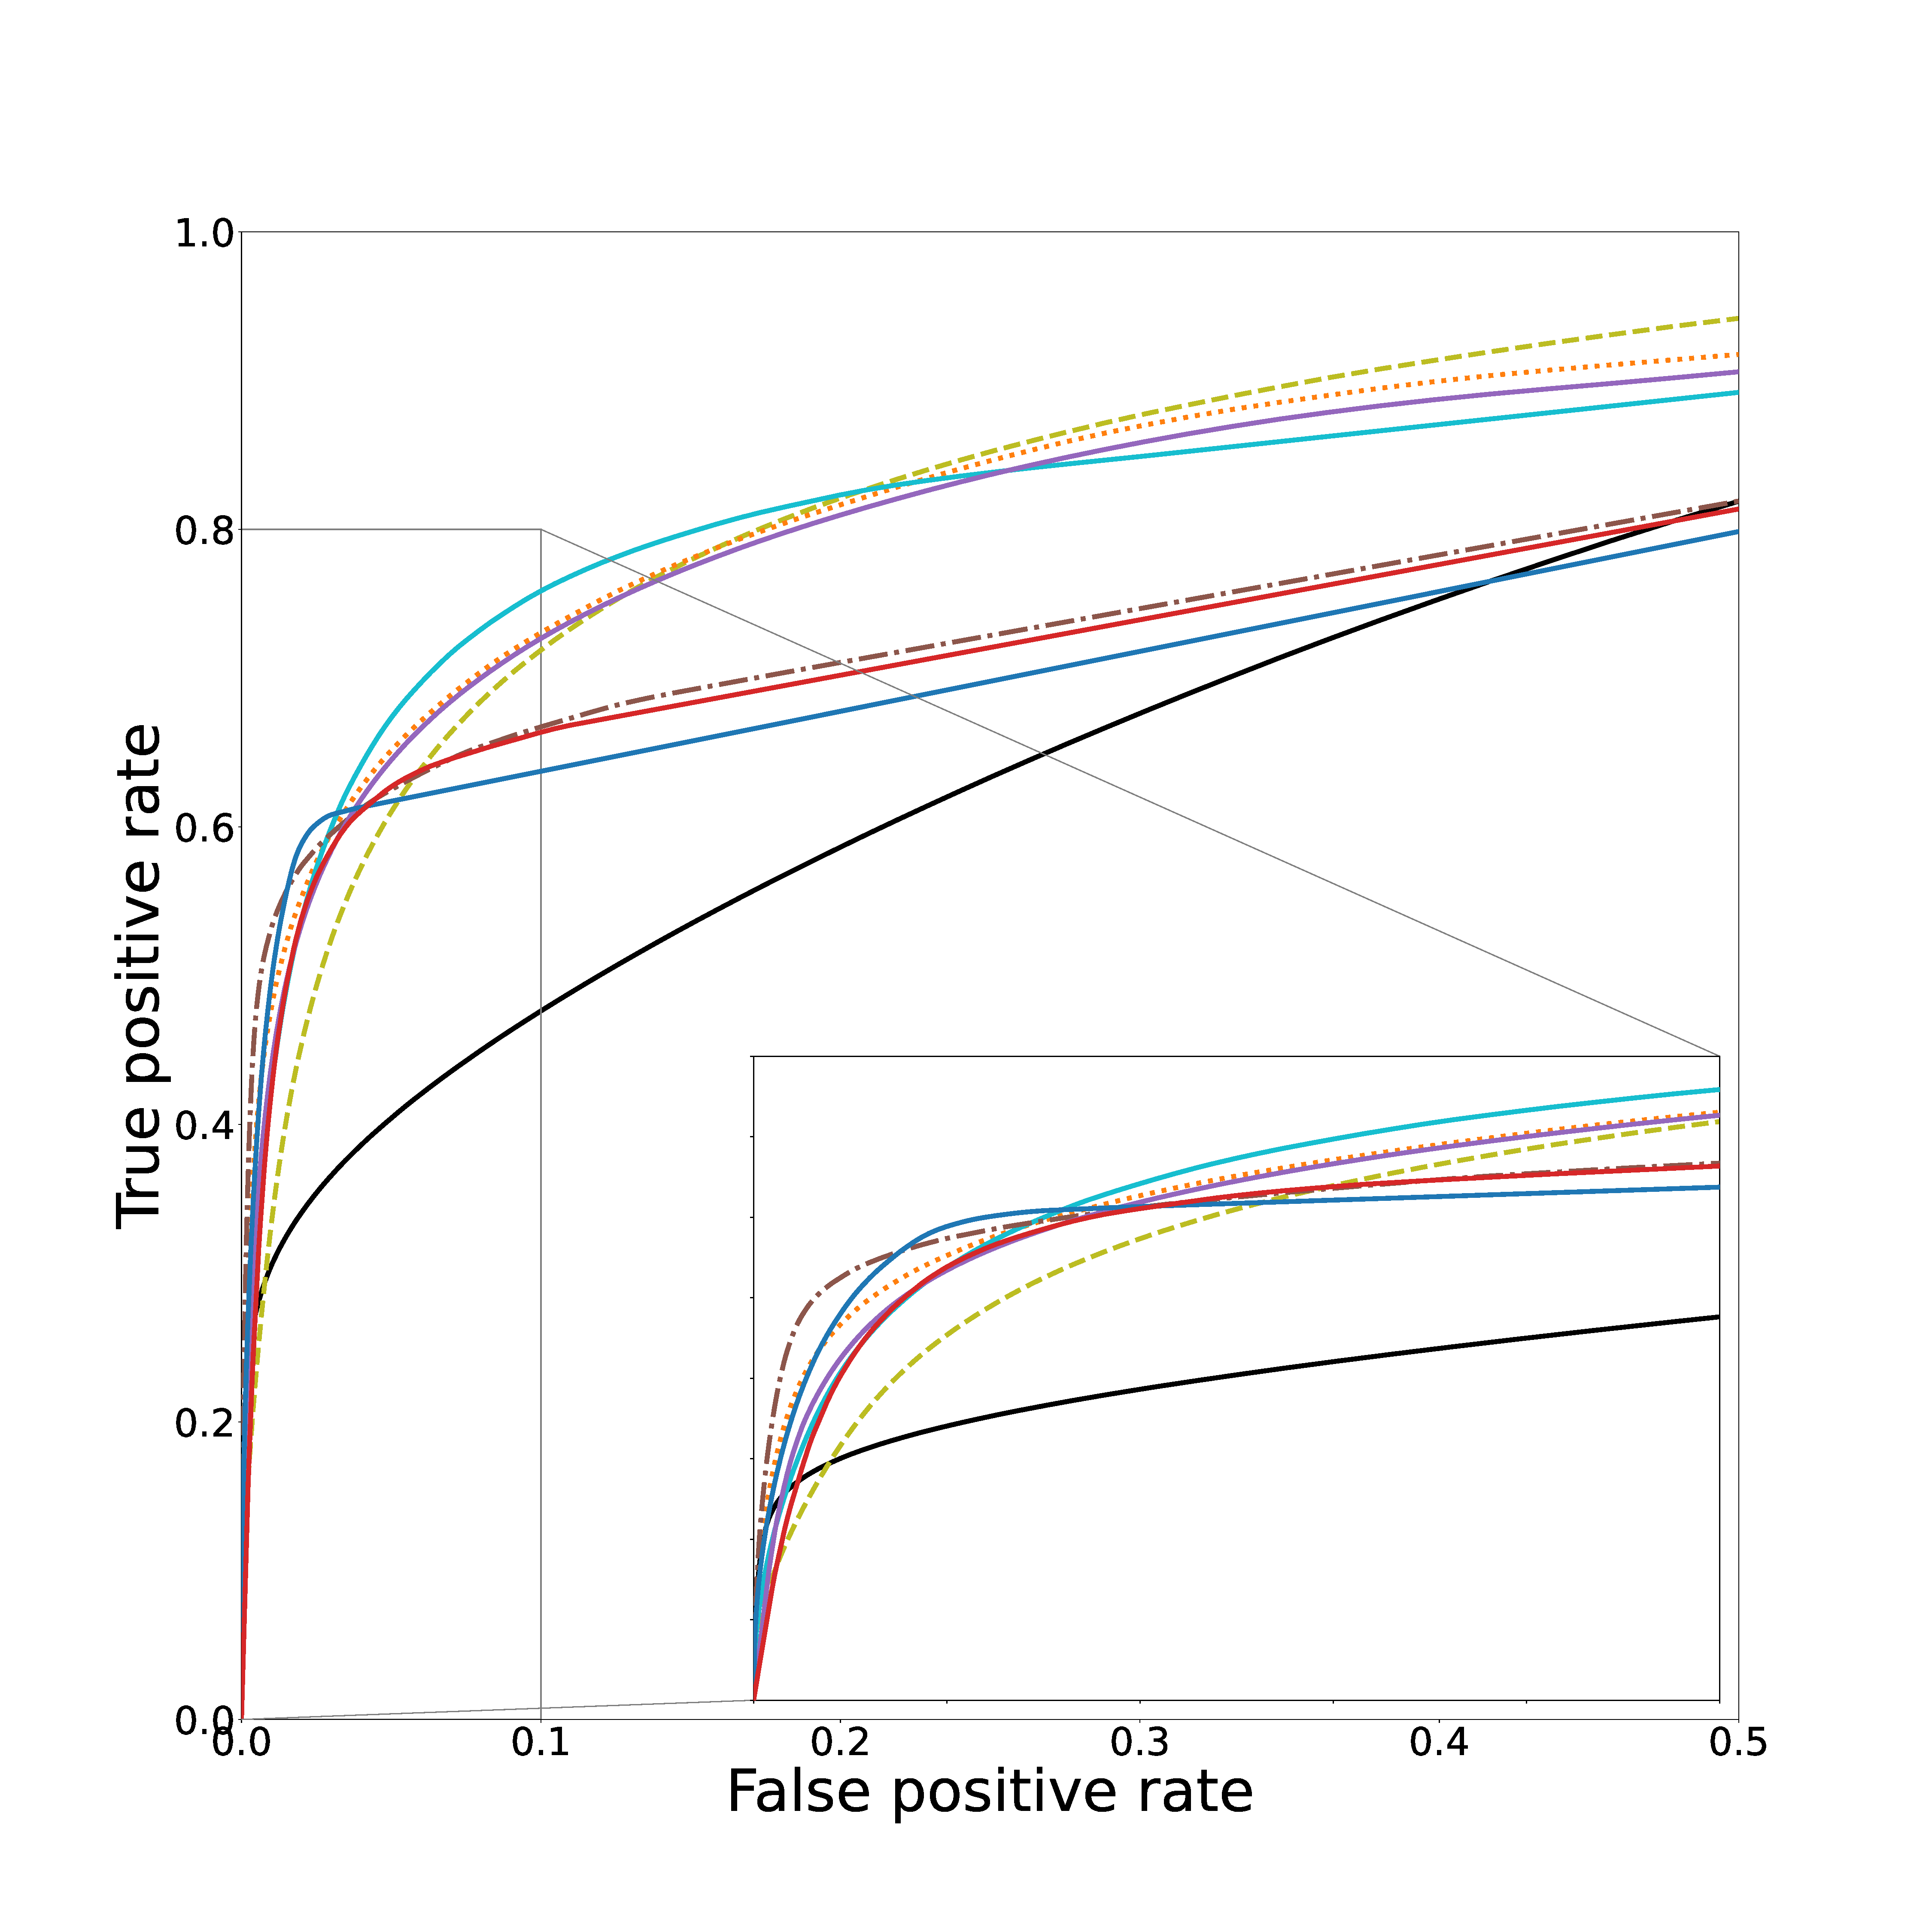
\includegraphics[clip = true, trim  =  125 125 180 200, height=9cm]{Images/Bullitt_ROC.pdf}
  \caption{Bullitt}
  \end{subfigure}
  \caption{Courbe ROC moyenne des sept filtres de rehaussement pour Bullitt}
\end{figure}
\begin{figure}[!ht]
  \begin{subfigure}[t]{\textwidth}
    \centering
  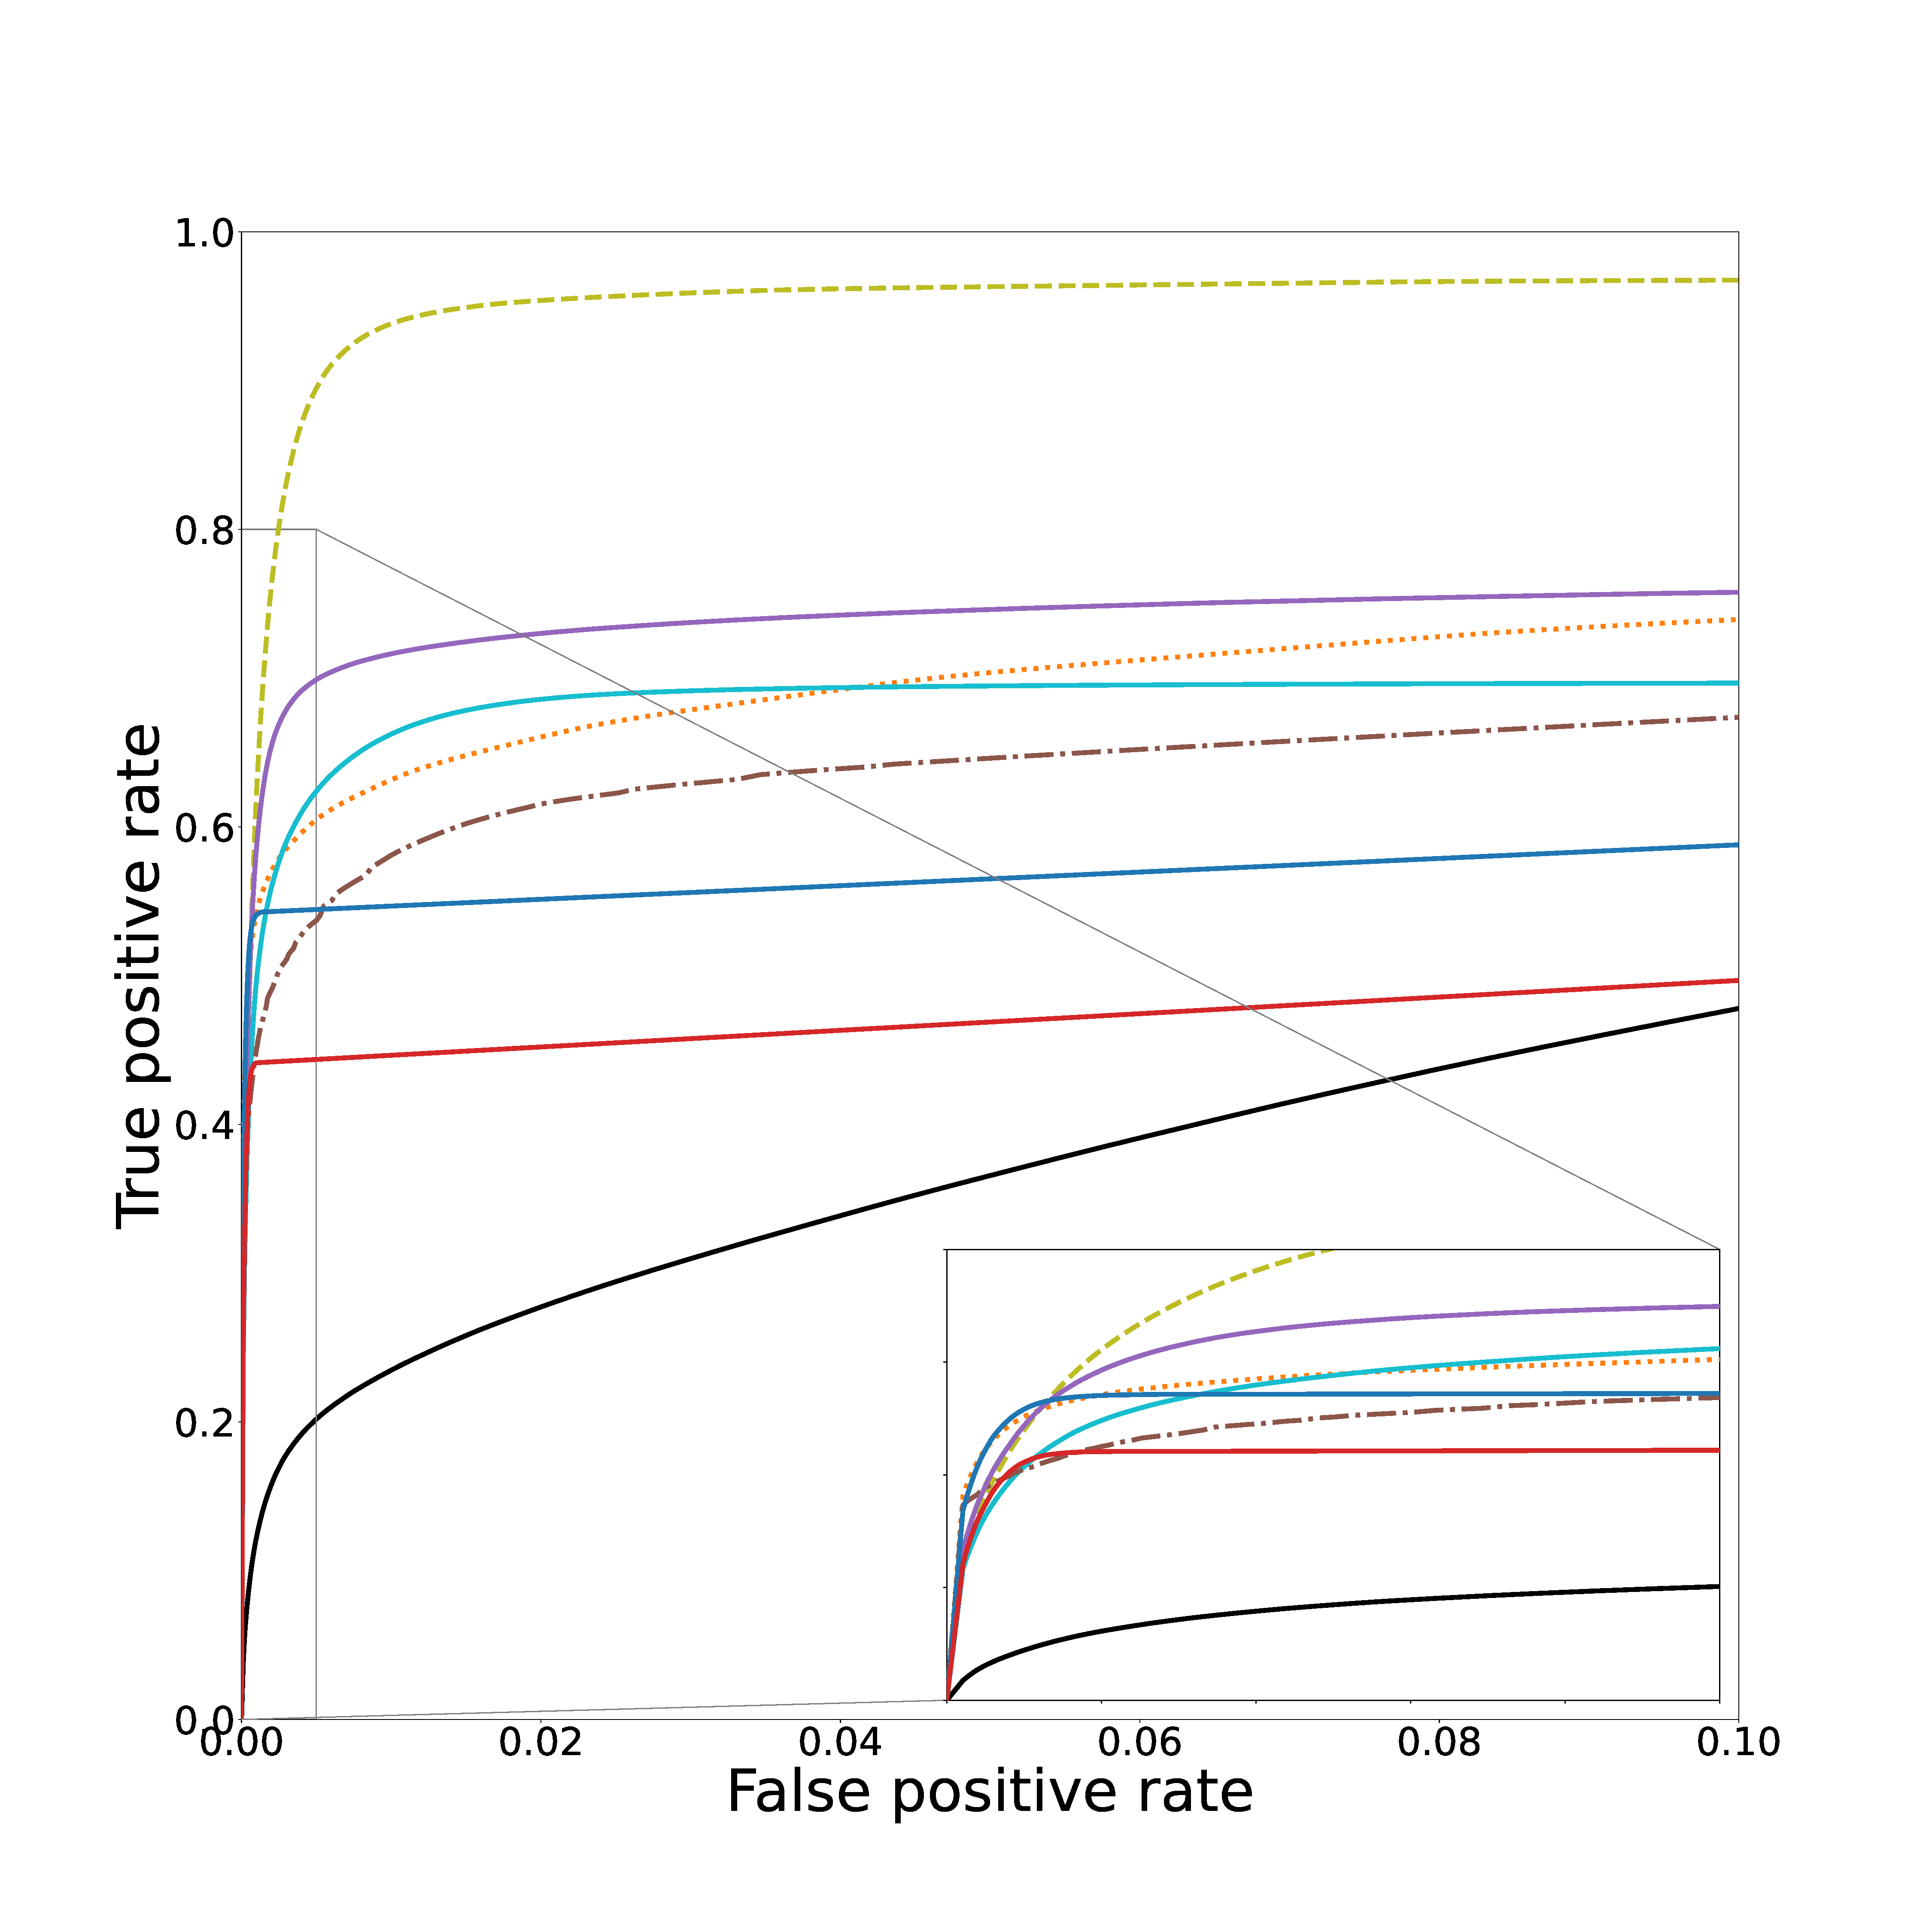
\includegraphics[clip = true, trim  =  125 125 100 200, height=9cm]{Images/Vascu_2_ROC.pdf}
  \caption{VascuSynth, $\sigma = 2$}
\end{subfigure}
\caption{Courbe ROC moyenne des sept filtres de rehaussement pour VascuSynth $\sigma=2$}
\end{figure}

\begin{figure}[!ht]
  \begin{subfigure}[t]{\textwidth}
    \centering
  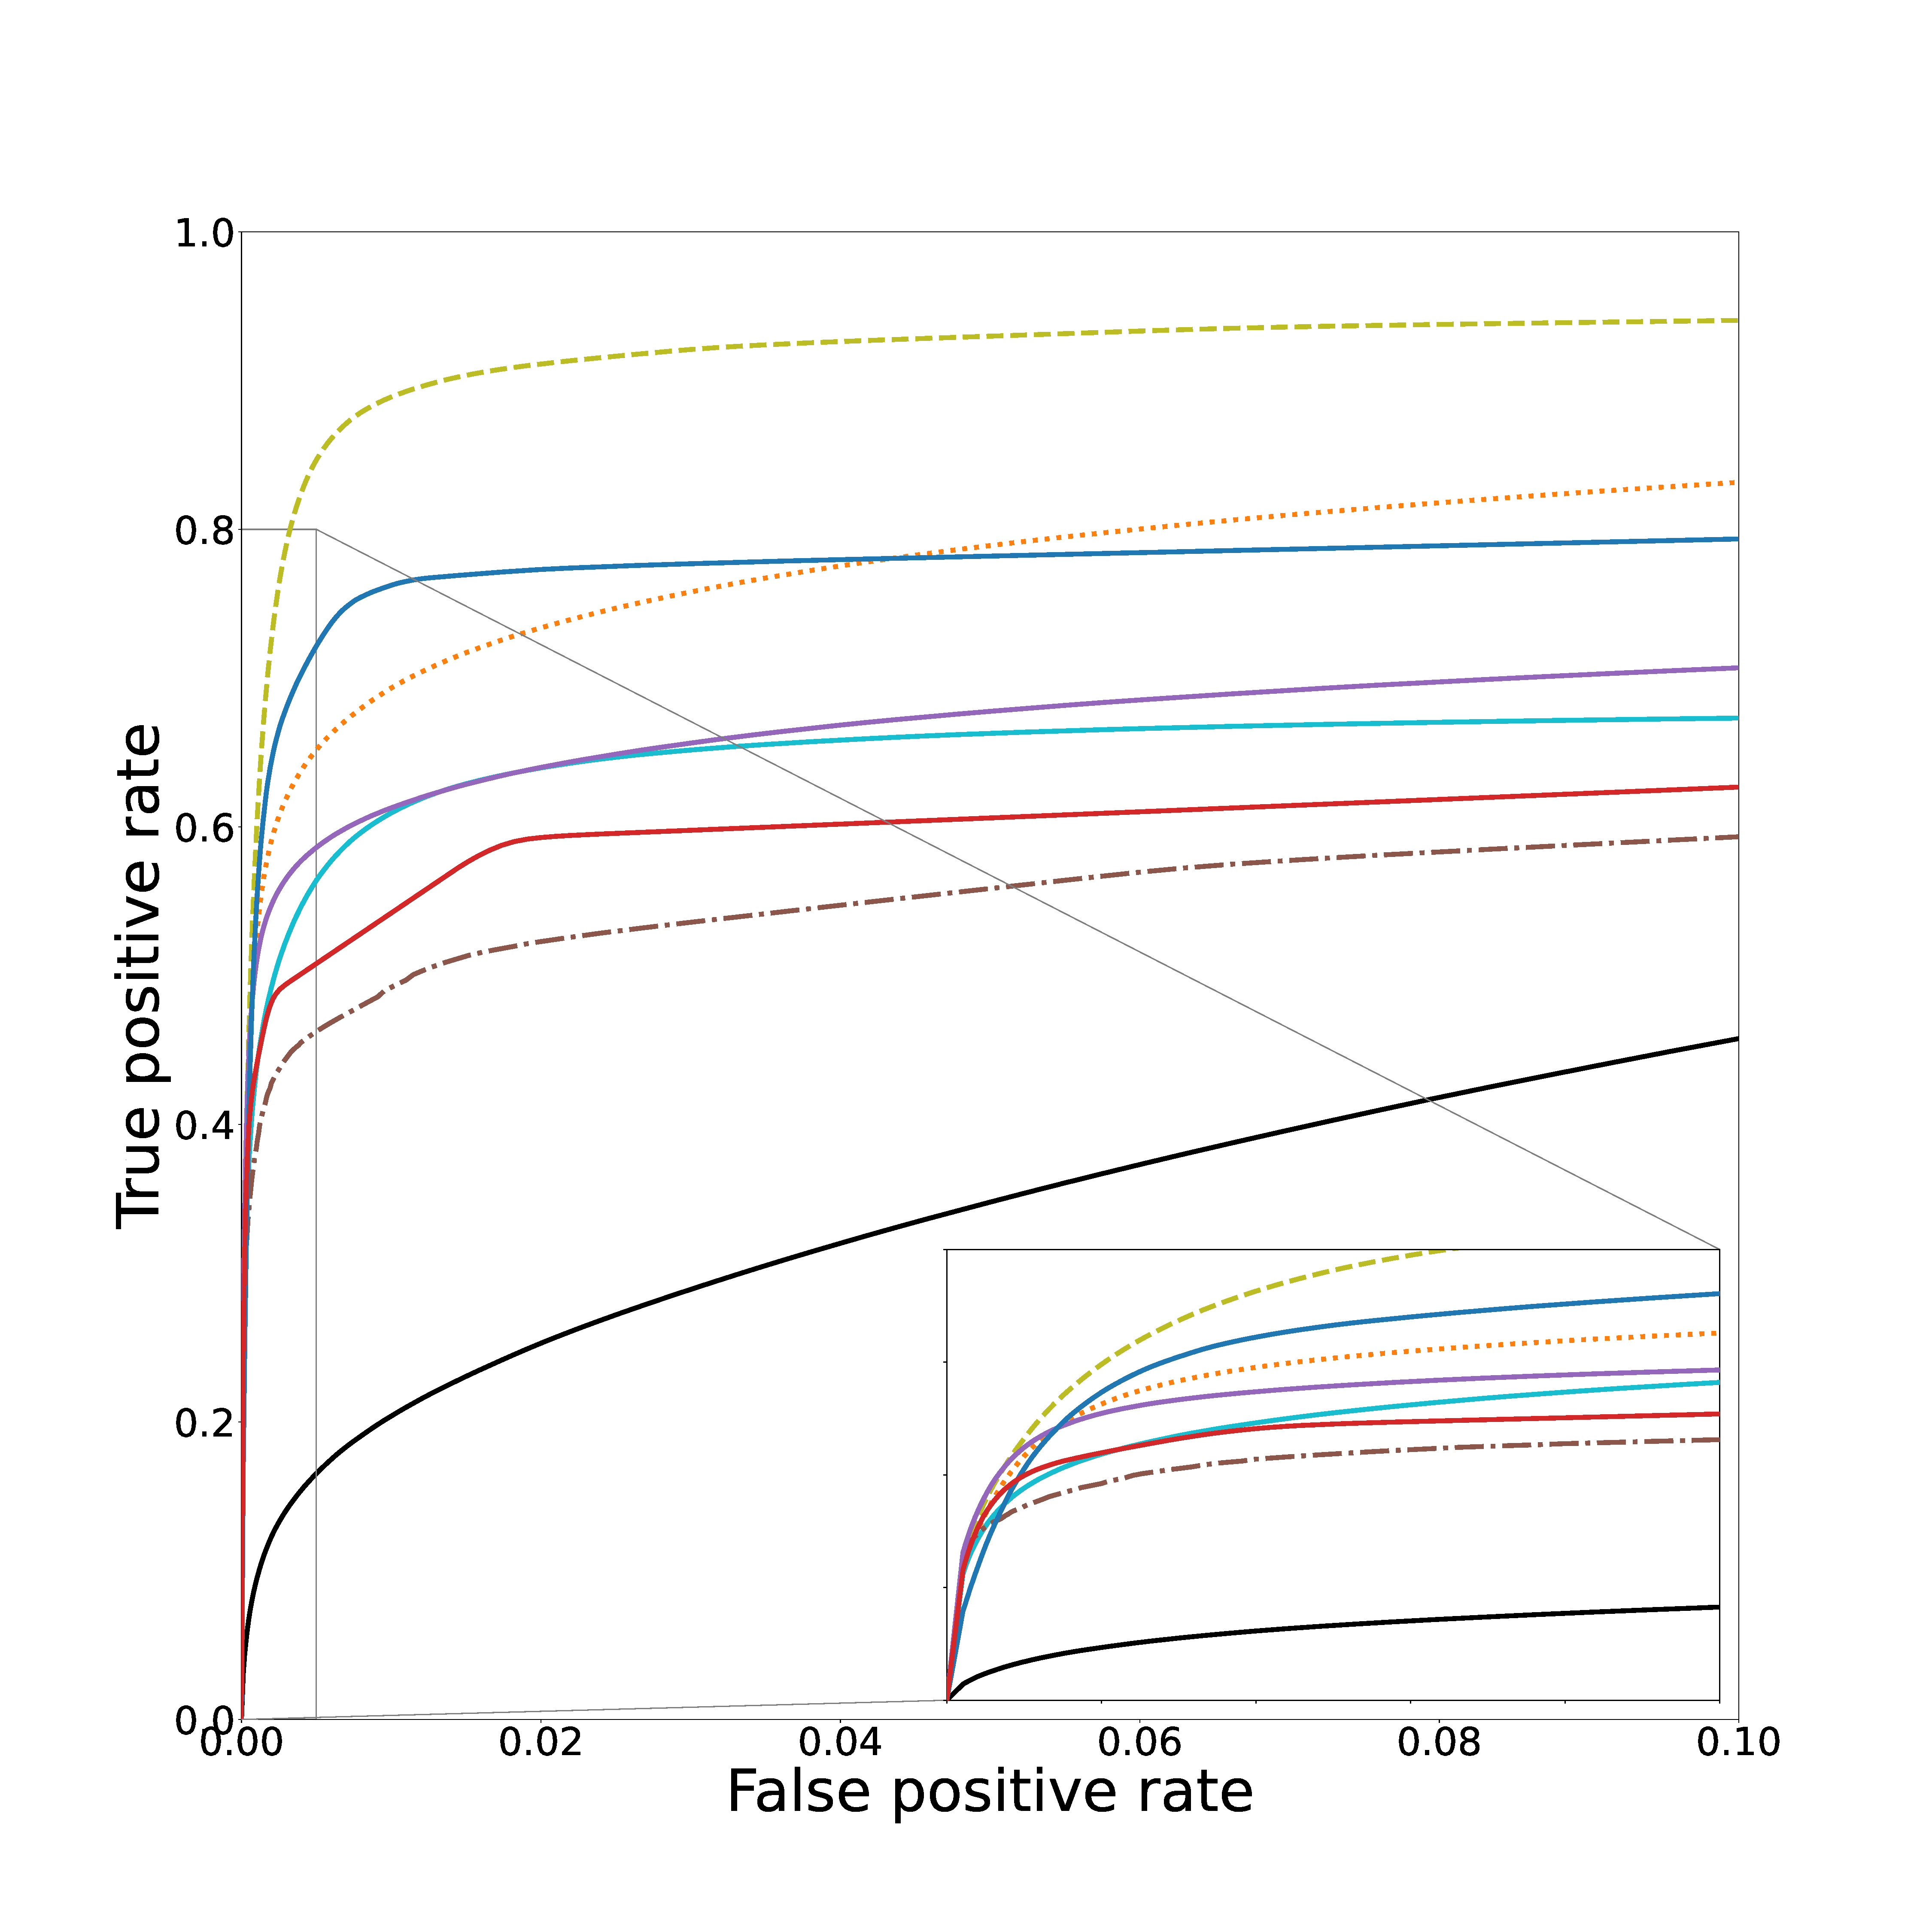
\includegraphics[clip = true, trim  =  125 125 100 200, height=9cm]{Images/Vascu_4_ROC.pdf}
  \caption{VascuSynth, $\sigma = 4$}
\end{subfigure}
\caption{Courbe ROC moyenne des sept filtres de rehaussement pour VascuSynth $\sigma=4$}
\end{figure}

\begin{figure}[H]
  \begin{subfigure}[t]{\textwidth}
    \centering
    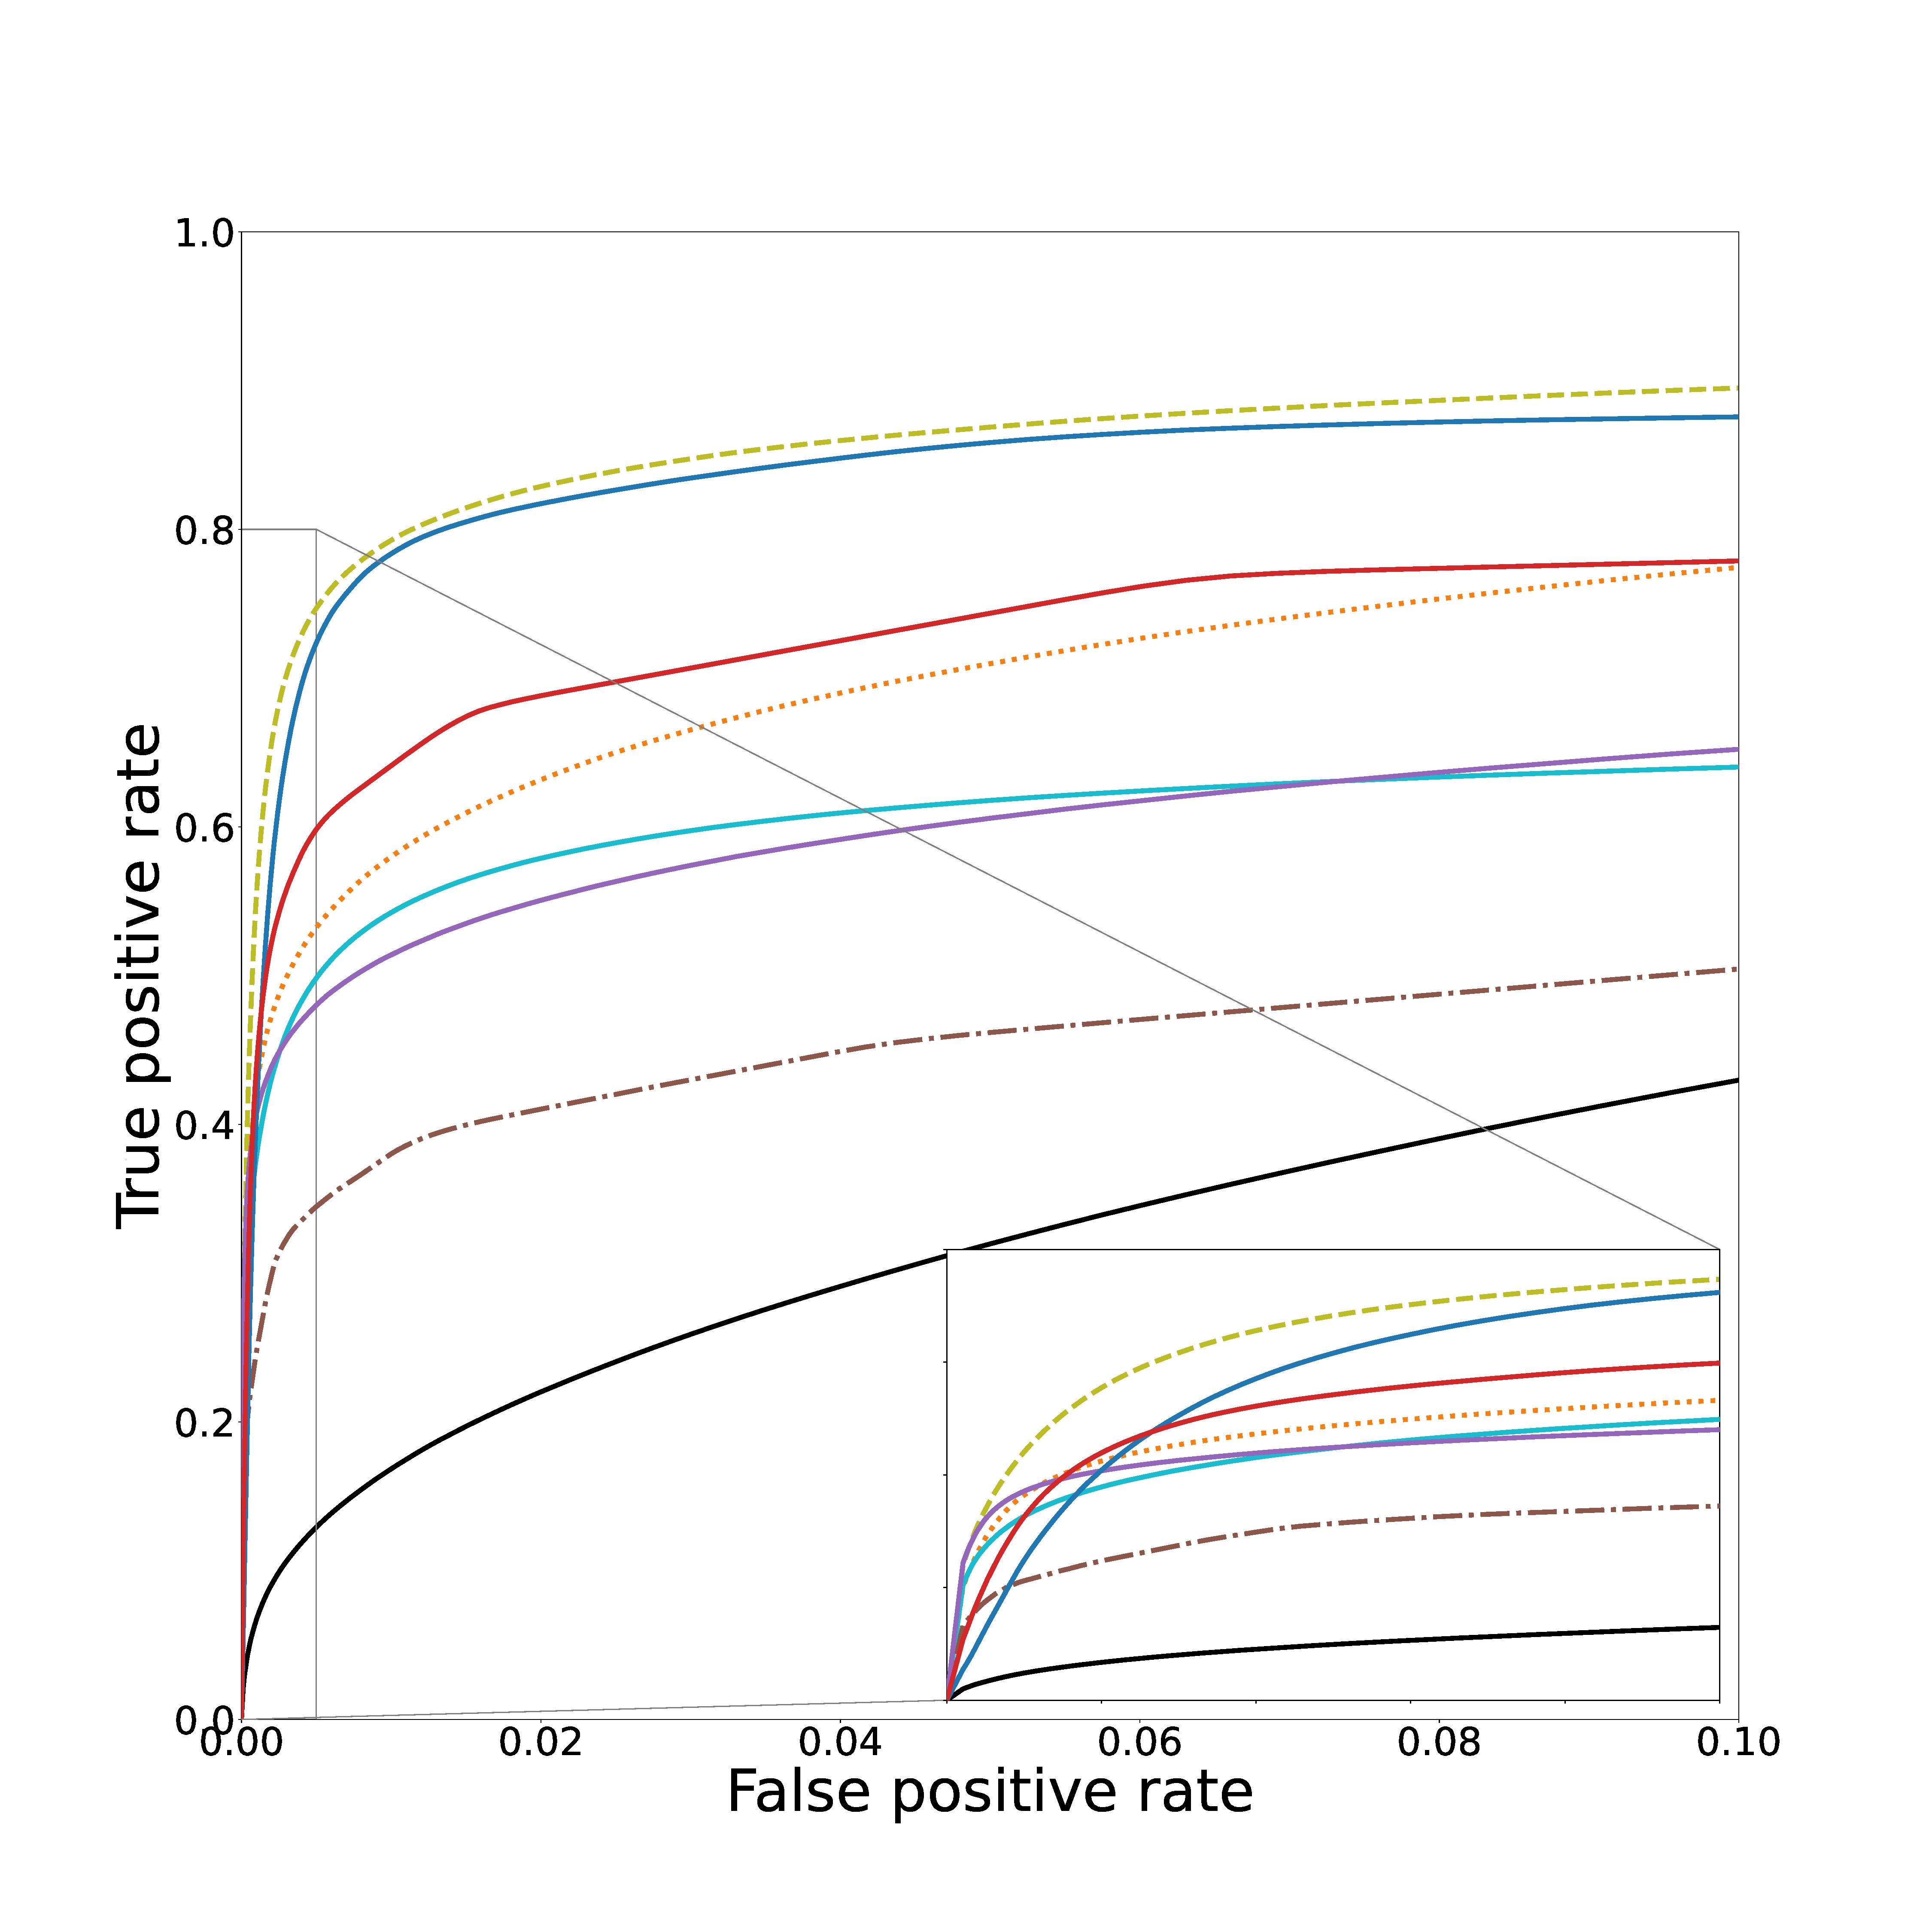
\includegraphics[clip = true, trim  =  125 125 100 200, height=9cm]{Images/Vascu_6_ROC.pdf}
    \caption{VascuSynth, $\sigma = 6$}
\end{subfigure}
\caption{Courbe ROC moyenne des sept filtres de rehaussement pour VascuSynth $\sigma=6$}
  \label{fig:Vascu6_ROC}
\end{figure}

\paragraph{Ircad}

\begin{table}[!ht]
  \begin{center}
      \caption{Résultats quantitatifs (moyenne $\pm$ écart-type) dans le masque global \maskglobal sur le jeu de données de l'Ircad.}
      \label{tab:quantitative results Ircad}
      \begin{tabular}{lccc}
          \hline
          & MCC & Dice & PSNR \\ 
          \hline
          Référence	& $ 0.452 \pm 0.129	$ & $ 0.468 \pm	0.126 $ & $	9.352  \pm  1.247 $ \\
          Frangi	    & $ 0.355 \pm 0.075	$ & $ 0.392 \pm	0.074 $ & $	19.899 \pm 	1.624 $ \\
          Jerman	    & $ 0.382 \pm 0.060	$ & $ 0.415 \pm	0.059 $ & $	18.926 \pm 	1.186 $ \\
          Meijering   & $ 0.232 \pm 0.036	$ & $ 0.241 \pm	0.050 $ & $	19.079 \pm 	1.392 $ \\
          OOF	        & $ 0.277 \pm 0.049	$ & $ 0.316 \pm	0.055 $ & $	19.728 \pm 	1.575 $ \\
          RORPO	    & $ 0.475 \pm 0.073	$ & $ 0.477 \pm	0.076 $ & $	20.349 \pm 	1.687 $ \\
          Sato	    & $ 0.340 \pm 0.056	$ & $ 0.380 \pm	0.057 $ & $	19.915 \pm 	1.633 $ \\
          Zhang	    & $ 0.434 \pm 0.085	$ & $ 0.462 \pm	0.079 $ & $	20.274 \pm 	1.648 $ \\
    
          \hline
      \end{tabular}  
      \end{center}    
\end{table}

En observant les résultats présentés en table \ref{tab:quantitative results Ircad}, on peut remarquer que globalement, le MCC et le Dice de tous les filtres appliqués sur les foies de l'Ircad sont faibles (inférieurs à 0.5). Ce résultat était attendu puisque nous avons réduit notre chaîne de traitement au minimum. Cependant, ce résultat justifie quantitativement le fait qu'un filtre seul ne peut se substituer à une méthode de segmentation complète.

Qualitativement (Fig. \ref{fig:qualitative results Ircad}), tous les filtres excepté RORPO produisent des faux positifs sur les bordures du foie. Meijering semble produire les moins bons résultats en rehaussant à la fois fortement les bordures et le bruit dans les tissus. En comparaison, la référence, permet de bien récupérer les vaisseaux larges, mais la qualité des vaisseaux décroît, avec une augmentation des déconnexions au fur et à mesure que les vaisseaux deviennent de plus en plus petits. 

Quantitativement, RORPO propose les meilleurs résultats avec un MCC de $0.475$. La référence à base de seuils obtient le second meilleur MCC ($0.452$). Le fait qu'un simple seuillage produise de meilleurs résultats que la plupart des filtres sur des images TDM injectées peut paraître étrange. Cependant, ces résultats sont à pondérer par le fait que les petits et moyens vaisseaux sont absents de la référence dans une proportion bien plus large que pour les filtres de rehaussement. En effet, tous les filtres ont des résultats supérieurs à la référence pour les moyens et petits vaisseaux.  

Zhang produit le troisième meilleur résultat (MCC = $0.434$), alors que OOF (MCC = $0.277$) et Meijering (MCC = $0.231$) présentent les performances les plus faibles. Les meilleurs filtres (RORPO et Zhang) obtiennent ces performances par des stratégies différentes. La précision de RORPO est élevée ($0.666$) avec une sensibilité moyenne ($0.379$). Au contraire, Zhang présente une sensitivité importante ($0.435$) en contrepartie d'une précision plus faible ($0.515$).

Nous rappelons que ces résultats sont basés sur le meilleur jeu de paramètres moyen pour l'ensemble des volumes du jeu de données. Le processus d'optimisation produit donc un rehaussement qui est le compromis entre rehausser au maximum les vaisseaux, limiter le bruit et limiter le rehaussement des structures qui ne sont pas des vaisseaux (telles que les bords du foie). 

\begin{figure}[!ht]
  \centering
  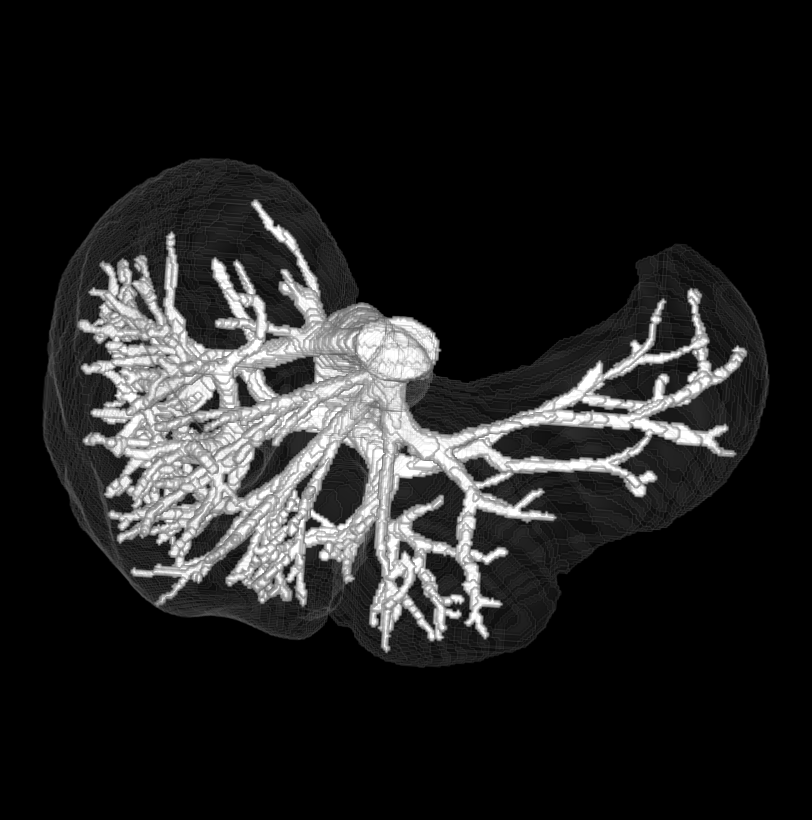
\includegraphics[clip = true, trim  =  10 150 10 150, height=3cm,width=4cm]{Images/Ircad_GT.png}
  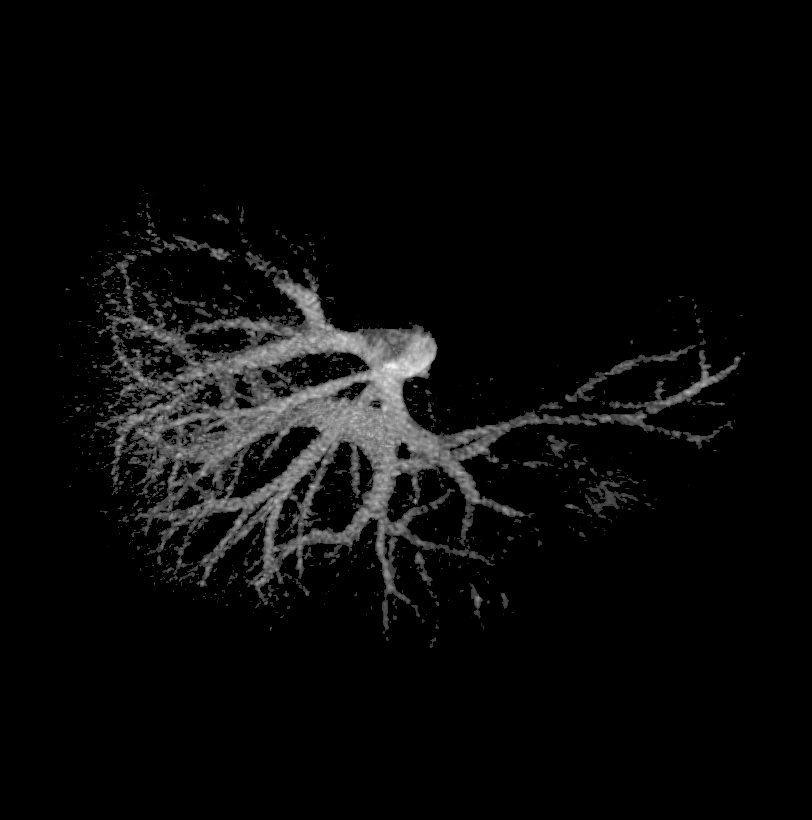
\includegraphics[clip = true, trim  =  10 150 10 150, height=3cm,width=4cm]{Images/Ircad_Baseline.png}
  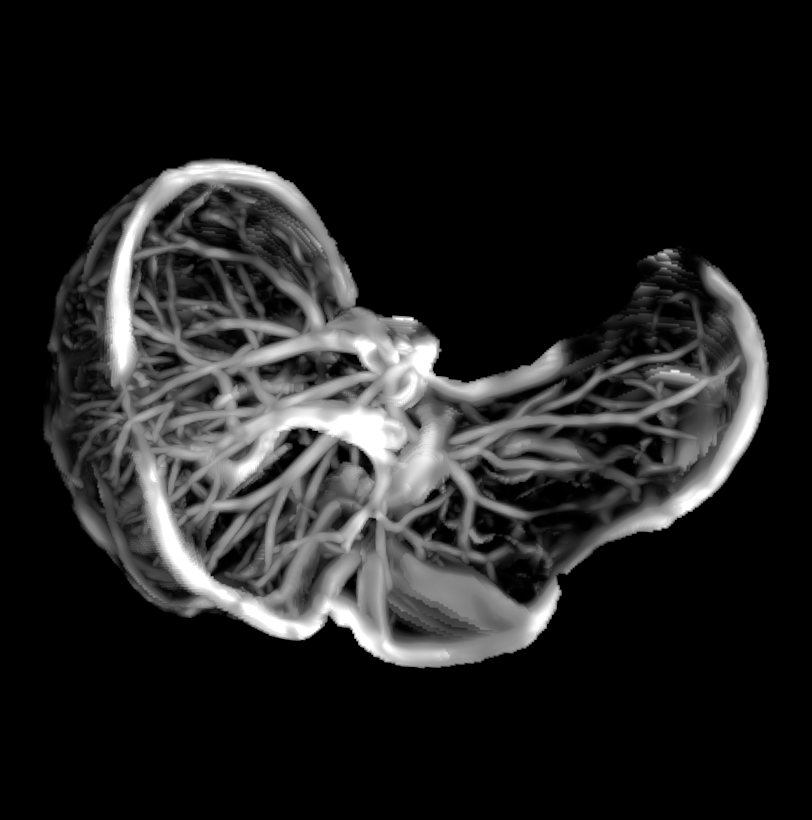
\includegraphics[clip = true, trim  =  10 150 10 150, height=3cm,width=4cm]{Images/Ircad_Frangi.png} \\
  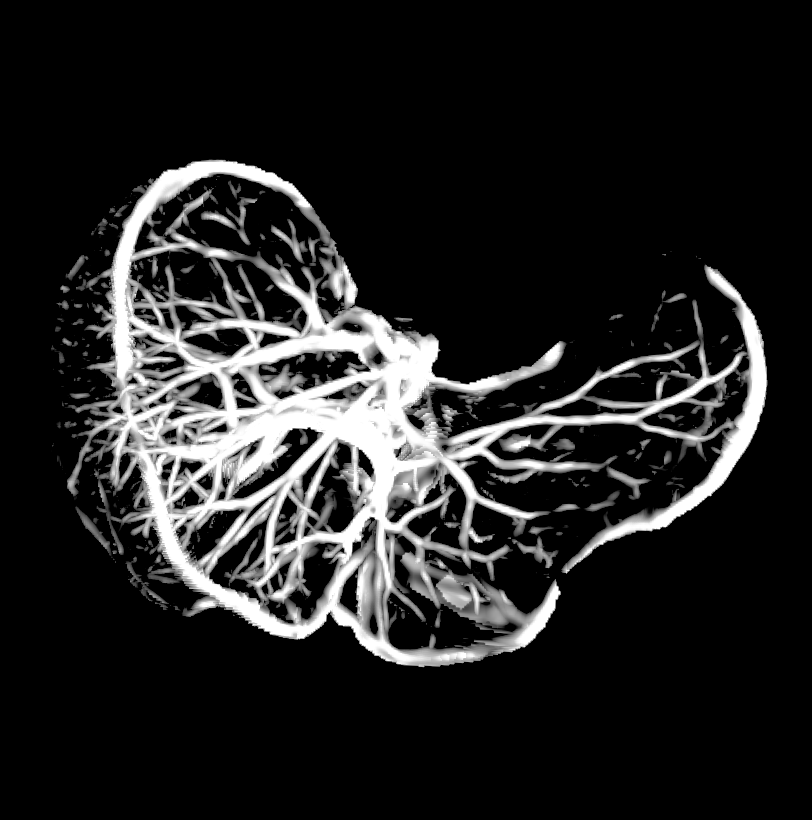
\includegraphics[clip = true, trim  =  10 150 10 150, height=3cm,width=4cm]{Images/Ircad_Jerman.png}
  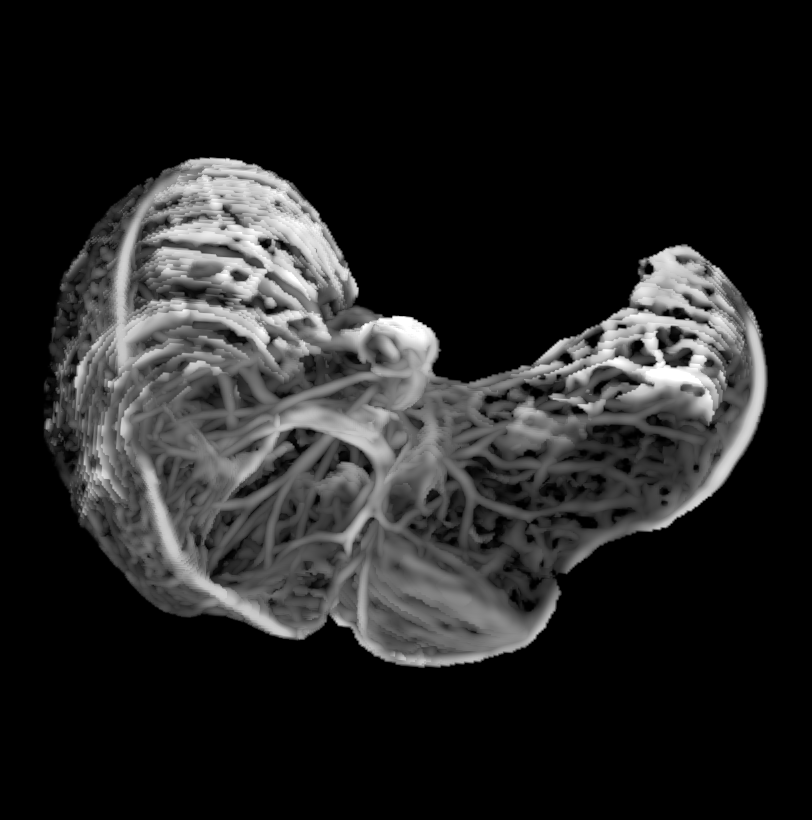
\includegraphics[clip = true, trim  =  10 150 10 150, height=3cm,width=4cm]{Images/Ircad_OOF_GM.png}
  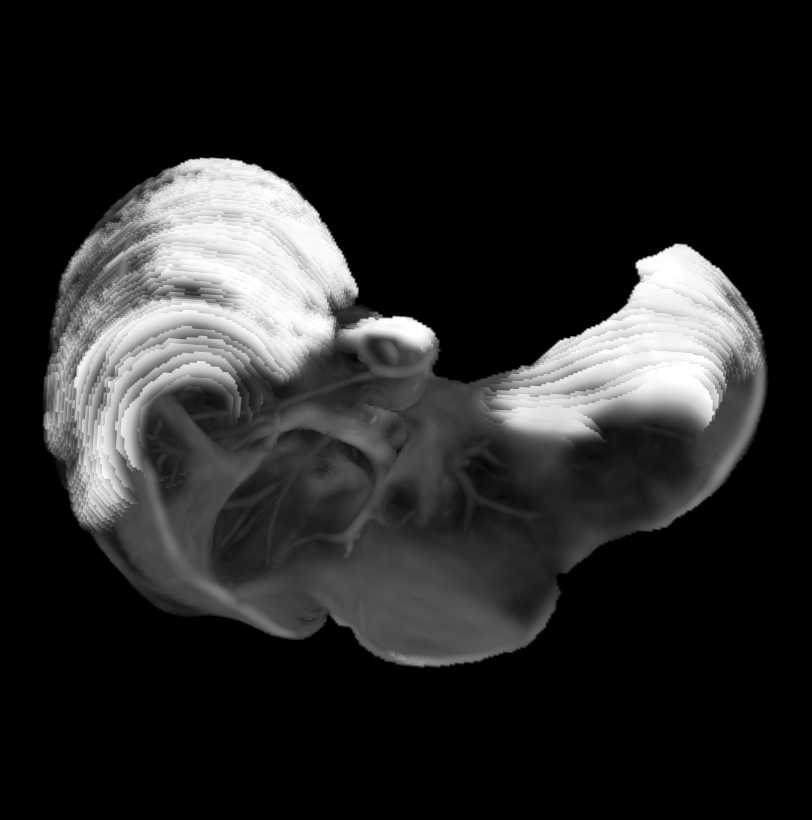
\includegraphics[clip = true, trim  =  10 150 10 150, height=3cm,width=4cm]{Images/Ircad_Meijering.png} \\
  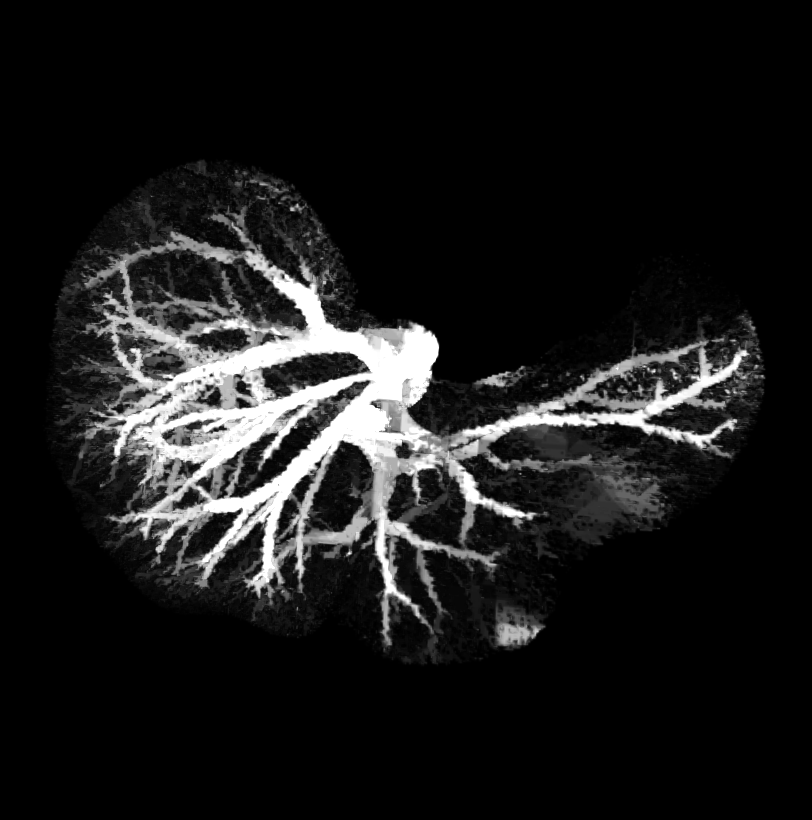
\includegraphics[clip = true, trim  =  10 150 10 150, height=3cm,width=4cm]{Images/Ircad_RORPO.png}
  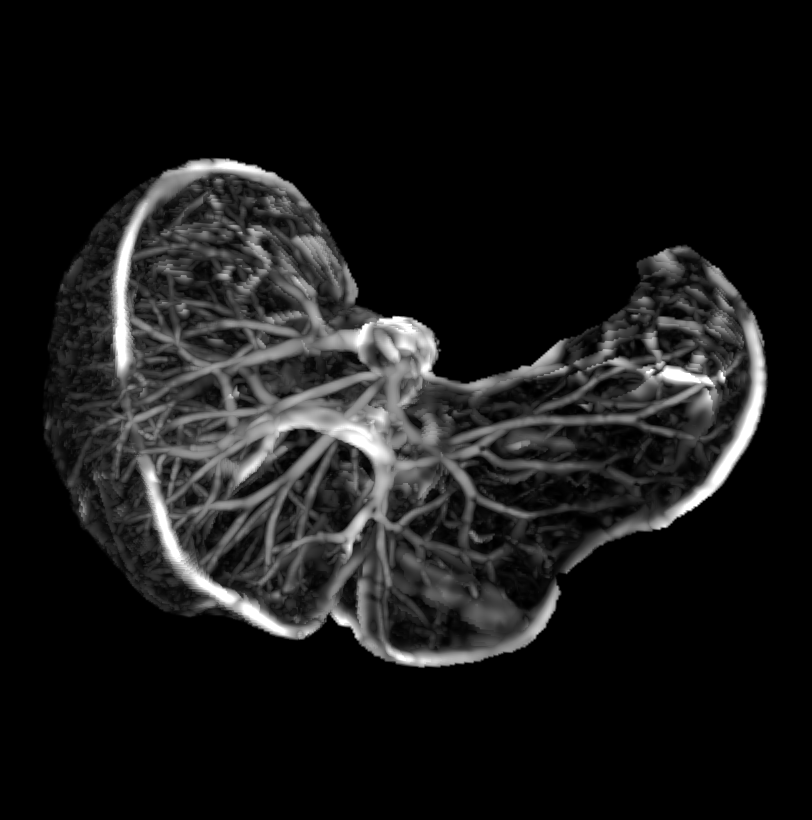
\includegraphics[clip = true, trim  =  10 150 10 150, height=3cm,width=4cm]{Images/Ircad_Sato.png}
  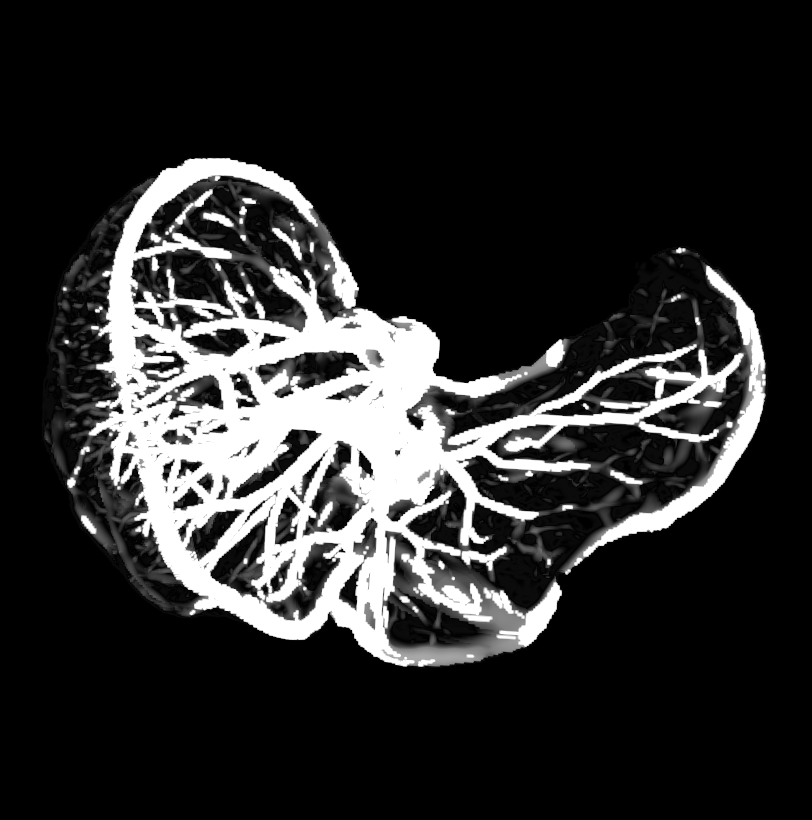
\includegraphics[clip = true, trim  =  10 150 10 150, height=3cm,width=4cm]{Images/Ircad_Zhang.png}
  \caption{Illustration des résultats de filtrage optimisé pour l'Ircad.
  Dans l'ordre de lecture vérités terrains, suivies de la référence, Frangi, Jerman, OOF, Meijering, RORPO, Sato et Zhang.}
  \label{fig:qualitative results Ircad}
\end{figure}

\paragraph{Bullitt}

\begin{table}[H]
  \begin{center}
      \caption{Résultats quantitatifs (moyenne $\pm$ écart-type) dans le masque global \maskglobal sur le jeu de données de Bullitt.}
      \label{tab:quantitative results Bullit}
  \begin{tabular}{lccc}
      \hline
          & MCC & Dice & PSNR \\ 
      \hline
      Référence	  & $ 0.396 \pm 0.049 $ & $ 0.340 \pm 0.061 $ & $ 20.275 \pm	0.732 $ \\ 
      Frangi	    & $ 0.474 \pm 0.027 $ & $ 0.481 \pm 0.026 $ & $ 21.768 \pm	0.510 $ \\ 
      Jerman	    & $ 0.432 \pm 0.030 $ & $ 0.438 \pm 0.029 $ & $ 19.723 \pm	1.051 $ \\ 
      Meijering	  & $ 0.349 \pm 0.040 $ & $ 0.354 \pm 0.043 $ & $ 21.905 \pm	0.463 $ \\ 
      OOF	        & $ 0.417 \pm 0.029 $ & $ 0.424 \pm 0.030 $ & $ 21.875 \pm	0.491 $ \\ 
      RORPO	      & $ \tbf{0.543} \pm 0.021 $ & $ \tbf{0.540} \pm 0.023 $ & $ \tbf{21.909} \pm	0.497 $ \\ 
      Sato	      & $ 0.475 \pm 0.026 $ & $ 0.473 \pm 0.028 $ & $ 21.799 \pm	0.466 $ \\ 
      Zhang	      & $ 0.423 \pm 0.037 $ & $ 0.431 \pm 0.037 $ & $ 21.261 \pm	0.847 $ \\ 

      \hline
  \end{tabular} 
\end{center}
\end{table}

Qualitativement (Fig. \ref{fig:qualitative results VascuSynth}), RORPO semble le mieux rehausser les vaisseaux avec peu de bruit. Cependant, les vaisseaux faiblement contrastés présentent des déconnexions irrégulières typiques des filtres anti-extensifs. Quelques méthodes rehaussent le bruit dans les tissus du cerveau plus que d'autres telles que Jerman, Sato, Meijering et OOF. Cependant, Jerman et Sato présentent des profils de vaisseaux bien plus contrastés que le bruit. Le diamètre des vaisseaux est surestimé par Jerman, Zhang, Meijering et dans une moindre mesure par OOF. Cela amène à la fusion de vaisseaux adjacents (voir Fig. \ref{fig:bifurcation_Bullitt}). Le rehaussement de Zhang est irrégulier avec certains vaisseaux très contrastés et d'autres plus faiblement contrastés. Cet effet est provoqué par la K-moyenne qui introduit un rehaussement dépendant de la classe associée aux pixels.

Nous attirons l'attention du lecteur sur le fait que nous n'avons pas observé d'artefacts liés au bord sur ce jeu de données puisque nous avons érodé le masque du cerveau de manière à exclure les veines non labélisées qui auraient biaisé nos métriques. 

Quantitativement, RORPO offre de meilleurs résultats par rapport aux autres filtres (MCC=$0.543$). Sato (MCC=$0.475$) et Frangi (MCC=$0.474$) arrivent respectivement en seconde et troisième position. Bien que présentant des MCC proches, le rappel de Frangi est meilleur que celui de Sato  ($0.469$ et $0.399$) mais avec un plus faible taux de précision ($0.498$ vs. $0.585$). Jerman (MCC=$0.432$), Zhang (MCC=$0.424$) et OOF (MCC=$0.417$) présentent des résultats supérieurs à la base de référence (MCC=$0.396$) tandis que Meijering produit un fort taux de faux positifs qui pénalise le MCC ($0.349$).

\begin{figure}[H]
  \centering
  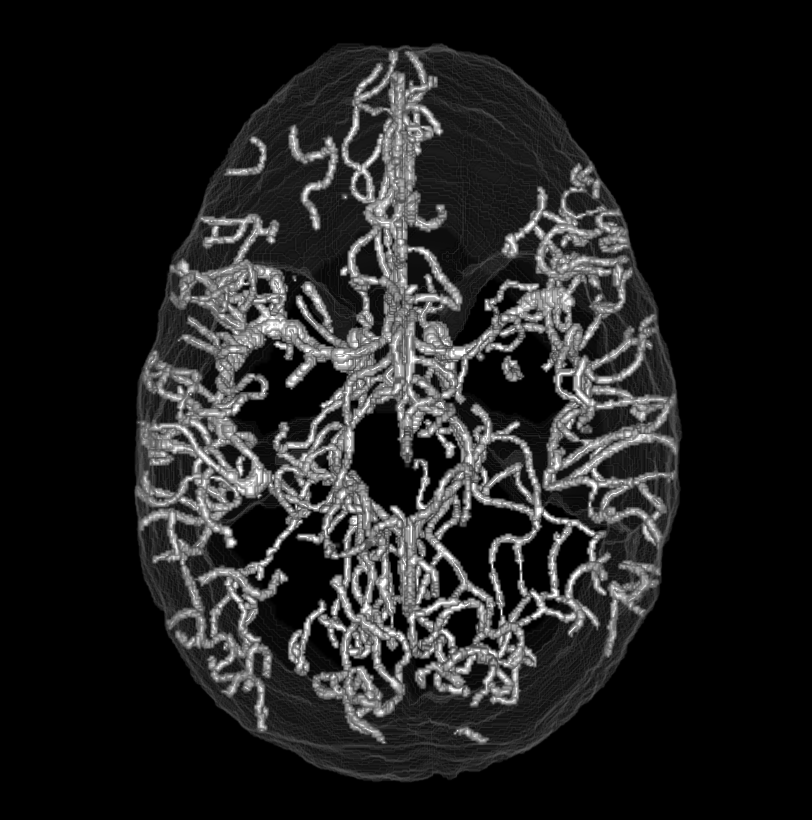
\includegraphics[clip = true, trim = 90 20 90 20, height=4cm,width=3.9cm]{Images/Bullitt_GT.png}
  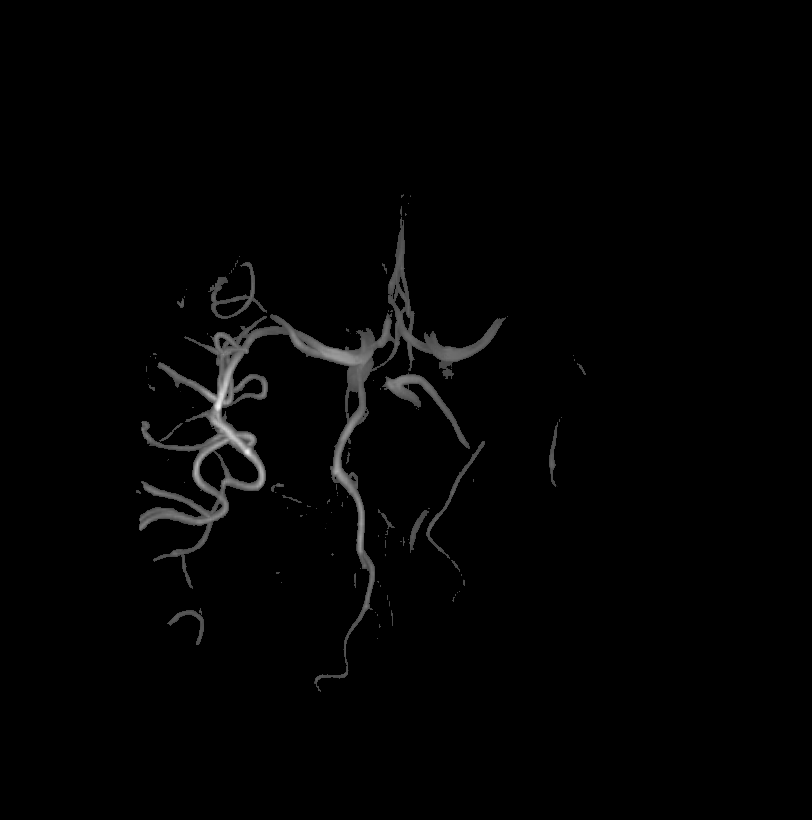
\includegraphics[clip = true, trim = 90 20 90 20, height=4cm,width=3.9cm]{Images/Bullitt_Baseline.png}
  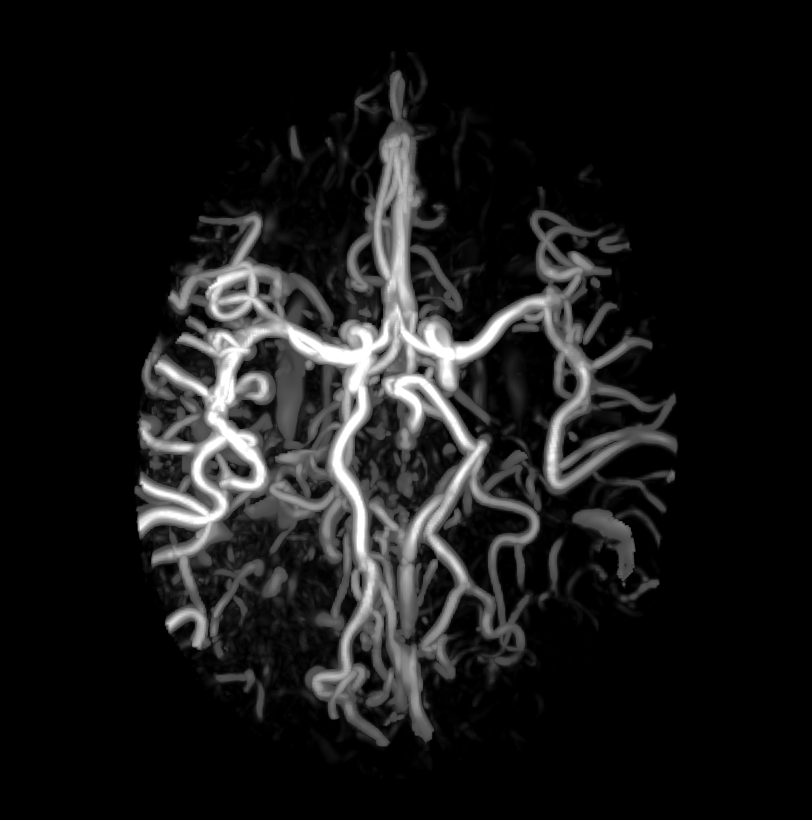
\includegraphics[clip = true, trim = 90 20 90 20, height=4cm,width=3.9cm]{Images/Bullitt_Frangi.png}
  \\
  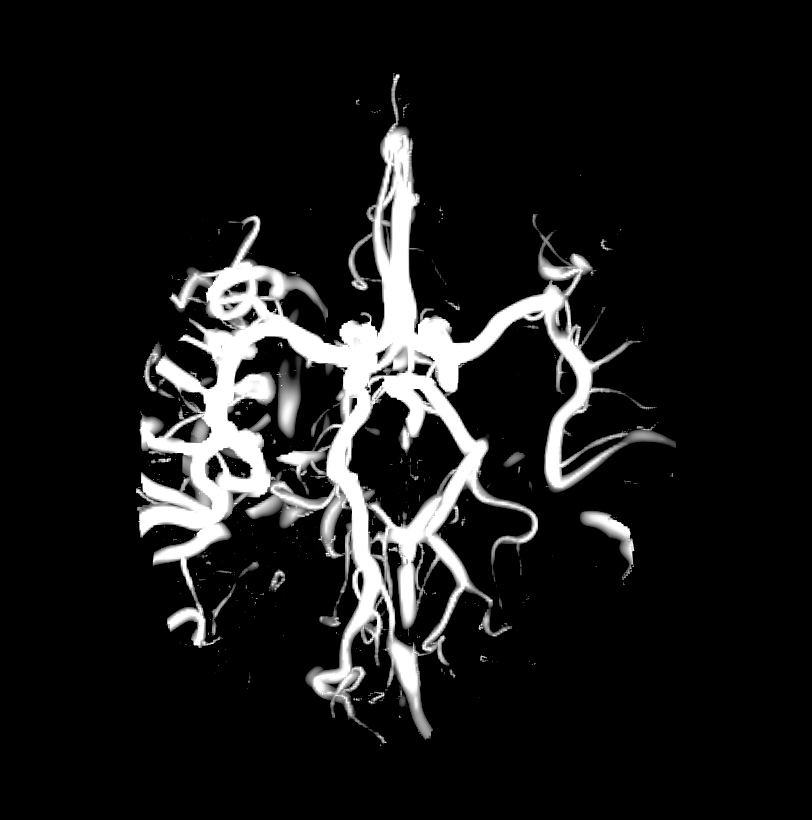
\includegraphics[clip = true, trim = 90 20 90 20, height=4cm,width=3.9cm]{Images/Bullitt_Jerman.png}
  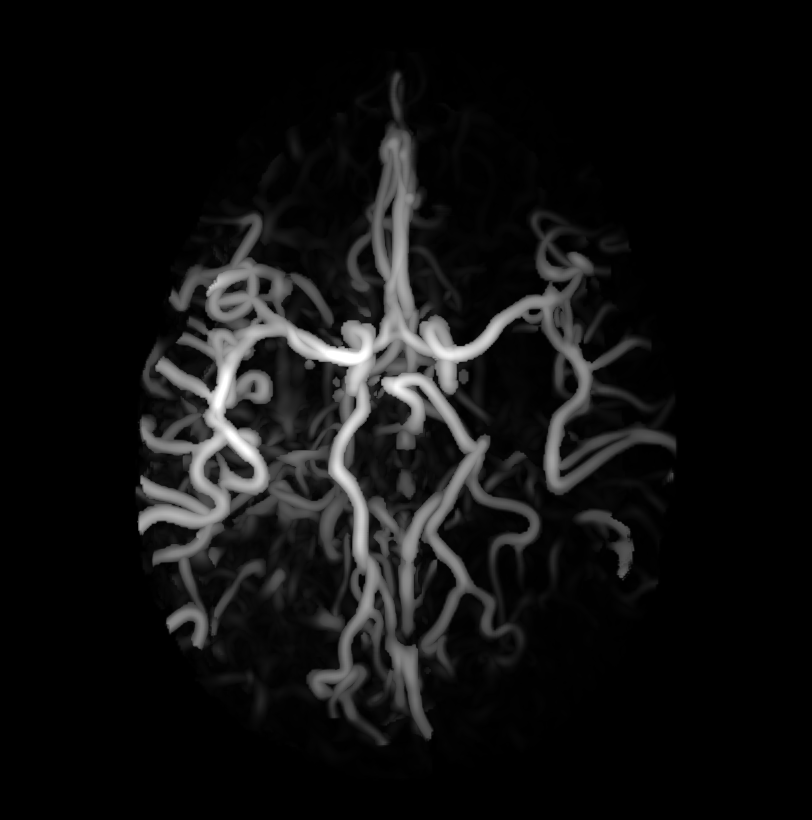
\includegraphics[clip = true, trim = 90 20 90 20, height=4cm,width=3.9cm]{Images/Bullitt_OOF_GM.png}
  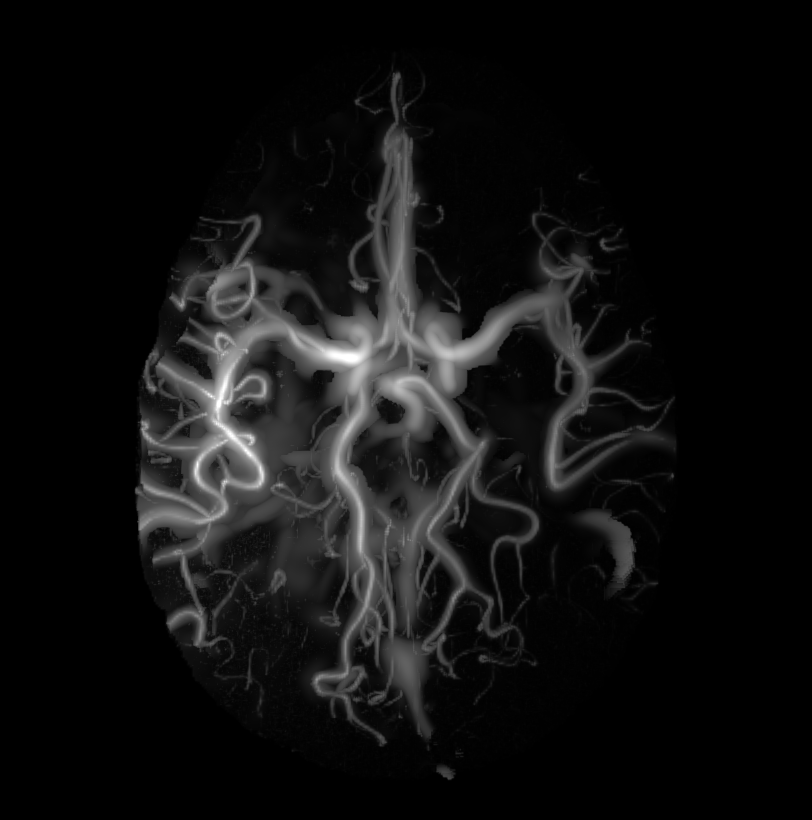
\includegraphics[clip = true, trim = 90 20 90 20, height=4cm,width=3.9cm]{Images/Bullitt_Meijering.png}
  \\
  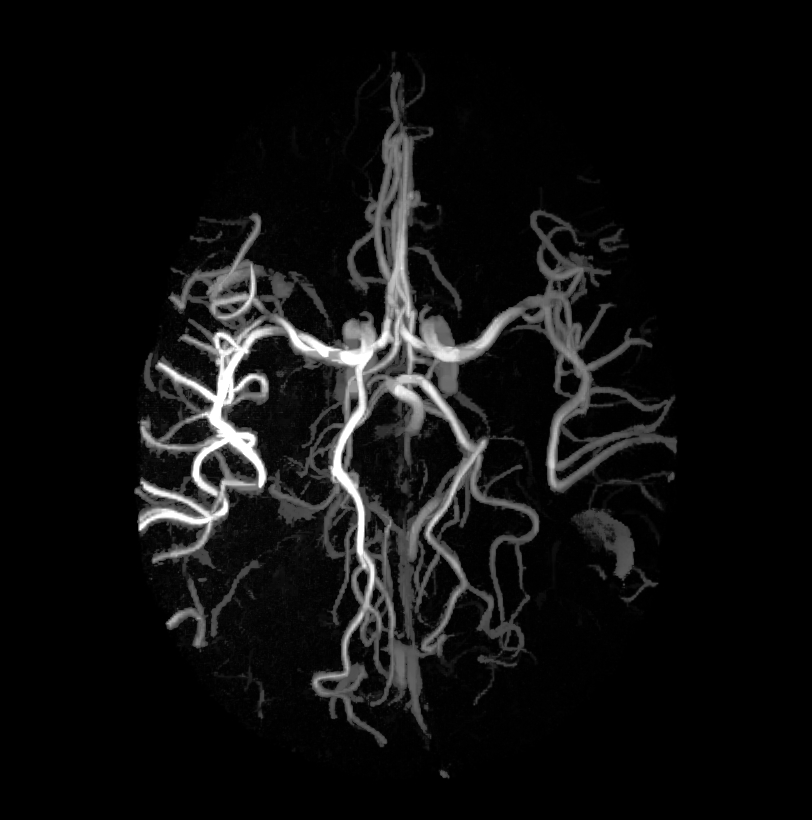
\includegraphics[clip = true, trim = 90 20 90 20, height=4cm,width=3.9cm]{Images/Bullitt_RORPO.png}
  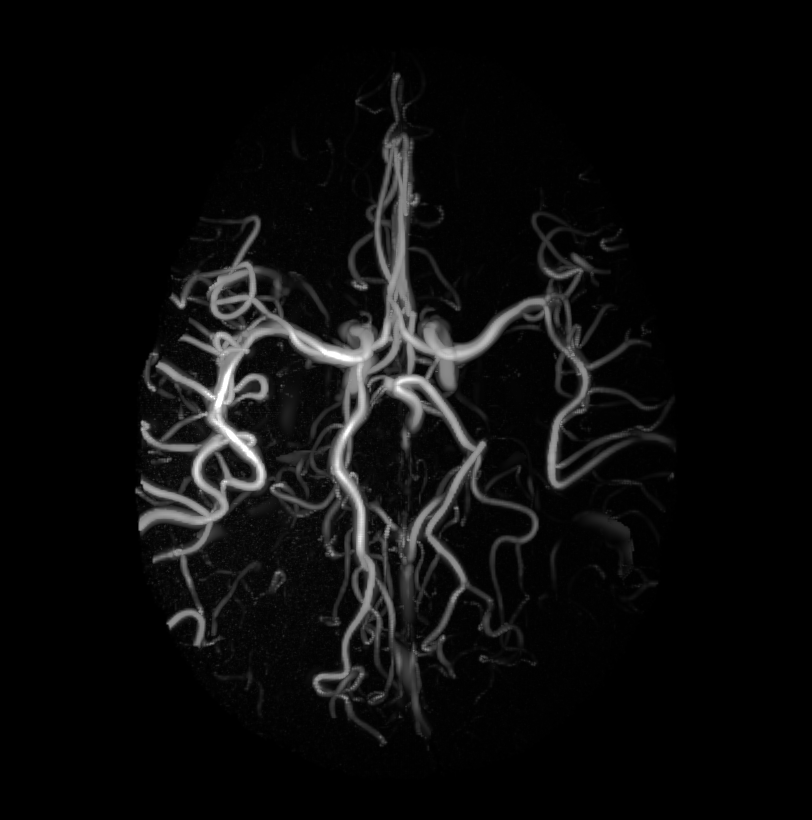
\includegraphics[clip = true, trim = 90 20 90 20, height=4cm,width=3.9cm]{Images/Bullitt_Sato.png}
  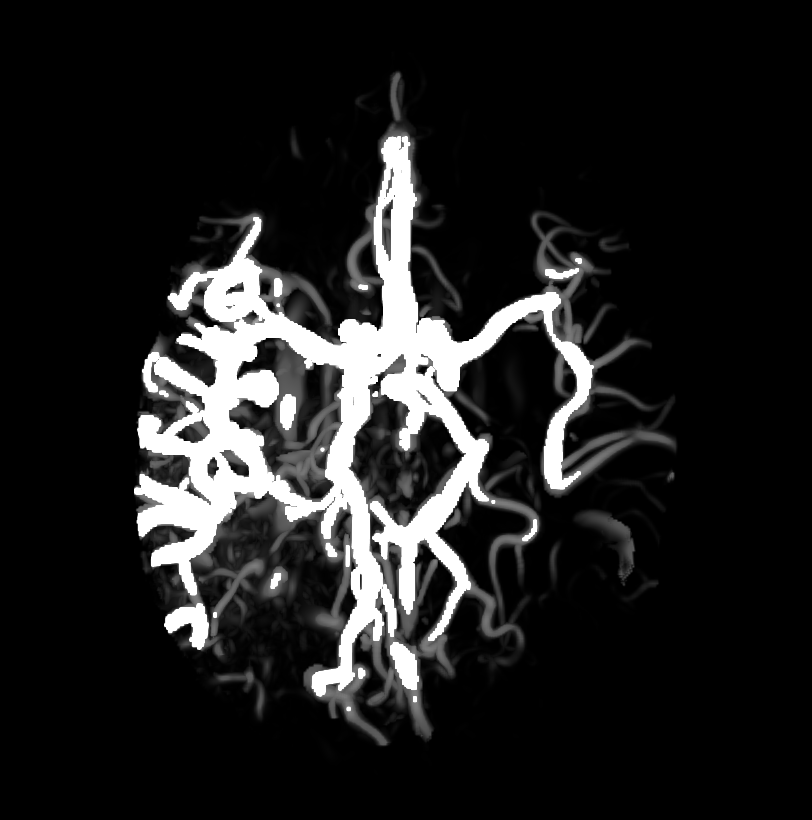
\includegraphics[clip = true, trim = 90 20 90 20, height=4cm,width=3.9cm]{Images/Bullitt_Zhang.png}
  \caption{Illustration des résultats de filtrage optimisé pour Bullitt.
  Dans l'ordre de lecture vérités terrains, suivies de la référence, Frangi, Jerman, OOF, Meijering, RORPO, Sato et Zhang.}
  \label{fig:qualitative results VascuSynth}
\end{figure}

\paragraph{VascuSynth}


\begin{table}[H]
    \begin{center}
    \caption{Résultats quantitatifs (moyenne $\pm$ écart-type) dans le masque global \maskglobal sur les jeux de données de VascuSynth.}
    \label{Table:quantitative results Vascusynth}
    \resizebox{\textwidth}{!}{
    \begin{tabular}{l|ccc|ccc|ccc}
    \hline
          & \multicolumn{3}{c|}{MCC} & \multicolumn{3}{c|}{Dice} & \multicolumn{3}{c}{PSNR} \\
          & $\sigma = 2$ & $\sigma = 4$ & $\sigma = 6$ & $\sigma = 2$ & $\sigma = 4$ & $\sigma = 6$ & $\sigma = 2$ & $\sigma = 4$ & $\sigma = 6$\\
         \hline
         Baseline	  & $ 0.184 \pm 0.136 $  & $ 0.143 \pm 0.116 $ & $ 0.106 \pm	0.089 $ & $	0.162 \pm 0.134 $ & $ 0.122 \pm 0.114 $ & $	0.089 \pm  0.087 $ & $  9.411 \pm   0.231 $ & $  9.397  \pm 0.230 $ & $  9.374  \pm	0.229 $ \\
         Frangi	    & $ \tbf{0.634} \pm 0.051 $  & $ 0.577 \pm 0.070 $ & $ 0.500 \pm	0.081 $ & $	\tbf{0.621} \pm 0.049 $ & $ 0.572 \pm 0.074 $ & $	0.485 \pm  0.091 $ & $ 26.274 \pm 	2.813 $ & $\tbf{26.496}	\pm 2.872 $	& $ \tbf{26.692}	\pm 2.856 $ \\
         Jerman	    & $ 0.611 \pm 0.064 $  & $ 0.565 \pm 0.049 $ & $ 0.501 \pm	0.048 $ & $	0.603 \pm 0.065 $ & $ 0.549 \pm 0.046 $ & $	0.464 \pm  0.048 $ & $ \tbf{26.774} \pm 	1.296 $ & $	21.758	\pm 0.399 $	& $ 21.831	\pm 0.489 $ \\
         OOF	      & $ 0.627 \pm 0.061 $  & $ 0.496 \pm 0.065 $ & $ 0.449 \pm	0.069 $ & $	0.530 \pm 0.060 $ & $ 0.476 \pm 0.063 $ & $	0.419 \pm  0.067 $ & $ 26.324 \pm 	1.802 $ & $	24.594	\pm 1.329 $	& $ 22.983	\pm 1.072 $ \\
         Meijering	& $ 0.538 \pm 0.061 $  & $ \tbf{0.603} \pm 0.059 $ & $ \tbf{0.565} \pm	0.060 $ & $	0.619 \pm 0.064 $ & $ \tbf{0.599} \pm 0.061 $ & $	\tbf{0.564} \pm  0.059 $ & $ 26.586 \pm 	2.331 $ & $	25.902	\pm 1.889 $	& $ 24.821	\pm 1.395 $ \\
         RORPO	    & $ 0.587 \pm 0.155 $  & $ 0.517 \pm 0.119 $ & $ 0.366 \pm	0.123 $ & $	0.554 \pm 0.157 $ & $ 0.476 \pm 0.117 $ & $	0.325 \pm  0.113 $ & $ 23.236 \pm 	2.472 $ & $	20.672	\pm 1.689 $	& $ 18.372	\pm 1.571 $ \\
         Sato	      & $ 0.618 \pm 0.046 $  & $ 0.559 \pm 0.058 $ & $ 0.488 \pm	0.052 $ & $	0.596 \pm 0.044 $ & $ 0.548 \pm 0.058 $ & $	0.464 \pm  0.050 $ & $ 26.602 \pm 	2.539 $ & $	26.241	\pm 1.803 $	& $ 24.801	\pm 1.285 $ \\
         Zhang	    & $ 0.553 \pm 0.052 $  & $ 0.523 \pm 0.051 $ & $ 0.481 \pm	0.065 $ & $	0.531 \pm 0.051 $ & $ 0.498 \pm 0.049 $ & $	0.474 \pm  0.067 $ & $ 26.221 \pm 	2.805 $ & $	26.360	\pm 2.826 $	& $ 26.543	\pm 2.845 $ \\
   
    \end{tabular} }
    \end{center}
\end{table}

Qualitativement (Fig. \ref{fig:qualitative results VascuSynth}), Meijering, Sato et Jerman produisent les meilleurs résultats. Cependant, Meijering a tendance à rehausser le bruit au voisinage des vaisseaux, donnant à leur contour un aspect irrégulier. Jerman a un rehaussement des vaisseaux de bonne qualité, mais rehausse aussi une partie significative du bruit. Frangi, Zhang et Sato semblent être les meilleures méthodes pour filtrer le bruit ricien. 

\todo{Remarque de Bertrand : C’est pas logique si tu mentionnes que c’était attendue les détections de Blob plus importants pour rorpo sur le bruit mais tu mentionnes que c’est du au paramètre de gestion de déconnexion qui pas bougé. Le lien entre les deux est pas si direct.}
\todo{Demander l'avis d'Odyssée, car je n'ai plus la justification...}

Dans ce jeu de données, RORPO est plus sensible au bruit. Ainsi, plus le bruit est important, plus les artefacts en forme de blob sont rehaussés. 
Ce comportement était en partie attendu puisque nous n'avons pas utilisé le paramètre de dilatation de RORPO (qui gère les déconnexions liées au bruit) en le laissant à 0. Ce choix a été motivé par le fait que ce paramètre ne peut pas être optimisé séparément des paramètres d'échelles. Toutefois, Dans des applications réelles avec un fort niveau de bruit, l'étude de ce paramètre est indispensable. 

Comme le jeu de données VascuSynth ne présente pas de bords d'organes où d'artefacts similaires, l'éventualité d'un faux rehaussement lié à ces artefacts est limitée comparé aux jeux de données réels, excepté pour OOF qui rehausse les bordures de l'image assimilées à des plans. La mesure utilisée pour OOF distingue en effet mal les structures planaires des structures tubulaires. Une autre mesure de tubularité telle que la mesure de Frangi pourrait être utilisée pour éviter ce problème. Etrangement, quand le bruit n'est pas bien filtré, les filtres de rehaussements ont tendance à introduire de fausses structures tubulaires non présentes dans l'image d'origine (Fig. \ref{fig:noisy_tubes}).

\begin{figure}[H]
  \centering
  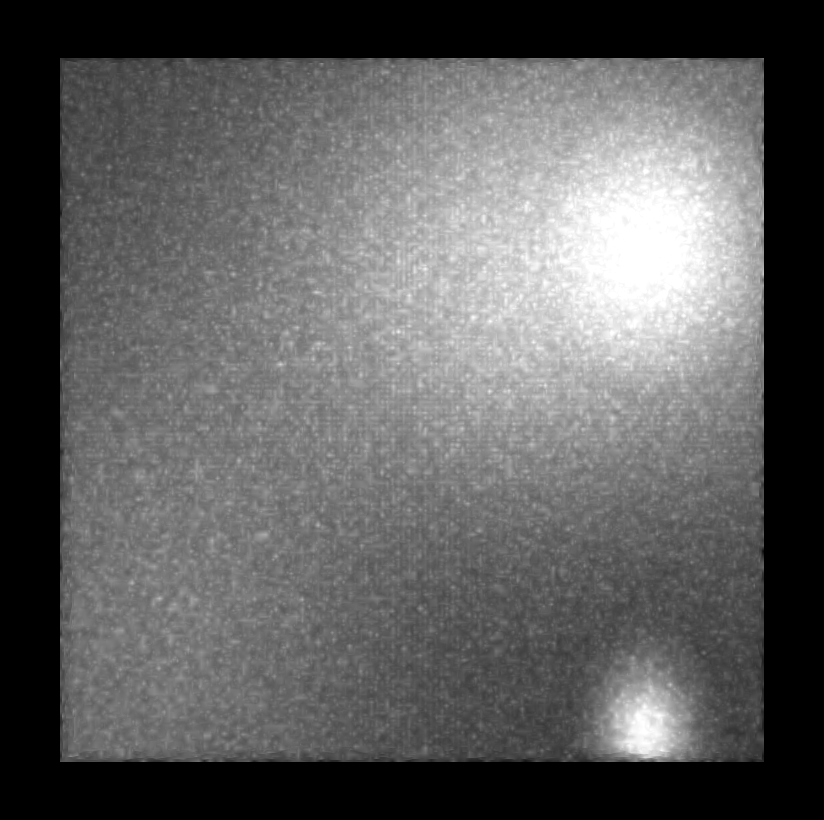
\includegraphics[height=4cm]{Images/vascu_noise.png}
  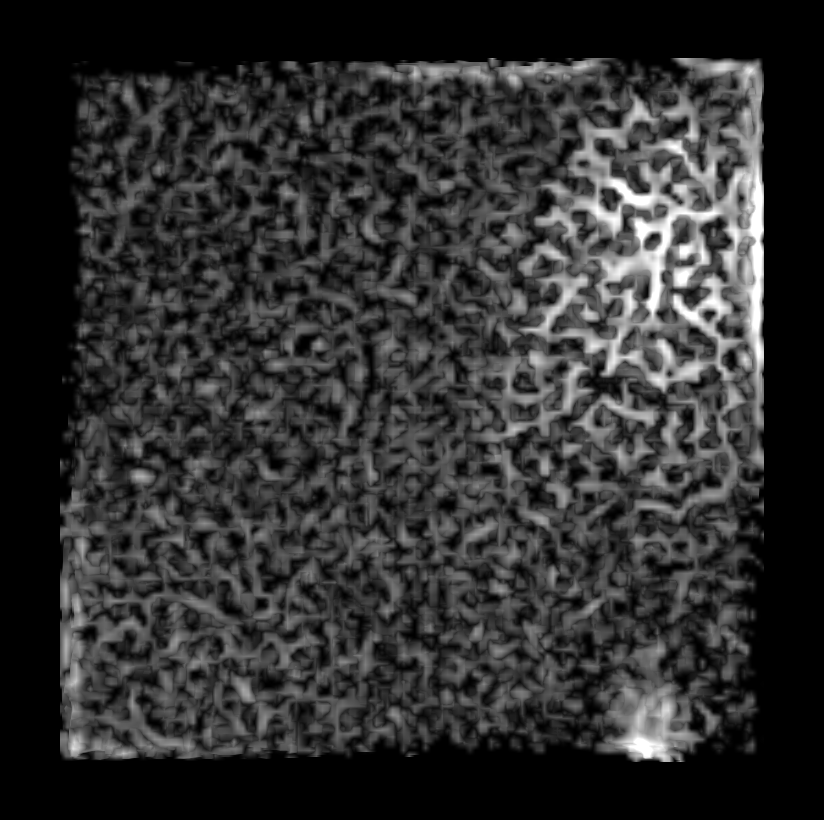
\includegraphics[height=4cm]{Images/vascu_noise_OOF.png}
  \caption{Bruit de fond de Vascusynth $\sigma=4$ et bruit de fond après filtrage par OOF.}
  \label{fig:noisy_tubes}
\end{figure}

Quantitativement, Frangi donne les meilleurs résultats pour $\sigma=2$ avec un MCC de $0.634$. Meijering  atteint un MCC de $0.603$ pour $\sigma=4$ et $0.565$ pour $\sigma=6$. Ces bonnes performances de Meijering peuvent s'expliquer par le fait que la géométrie des vaisseaux de VascuSynth corresponde aux hypothèses du modèle de Meijering (vaisseaux droits, et de rayon constant). Sato obtient le troisième meilleur résultat pour le niveau de bruit $\sigma=2$ (MCC=$0.618$) tandis que Jerman présente de meilleurs résultats pour des niveaux de bruits supérieurs (MCC = $0.565$ pour $\sigma=4$ et MCC=$0.501$ pour $\sigma = 6$). Peu importe les cas, les deux filtres donnent des résultats similaires, puisque leur sensibilité est proche, indépendamment du niveau de bruit. La différence entre les deux filtres s'explique au niveau de la précision : pour des niveaux de bruit élevés (e.g. $\sigma=4$), Jerman présente une plus grande précision (MCC = $0.717$ vs $0.661$) tandis que Sato présente une précision supérieure pour les faibles niveaux de bruit (MCC = $0.810$ vs. $0.689$). En général, Frangi est la méthode la plus robuste au bruit pour des niveaux de bruit élevés avec un PSNR de $26.496$ et $26.692$ pour $\sigma=4$ et $\sigma=6$, respectivement. Les résultats de la référence sont très mauvais à cause de la présence d'artefacts de haute intensité et d'un fond non homogène dans les données de VascuSynth. Ce comportement est une motivation supplémentaire pour l'usage de filtres de rehaussement pour des applications avec un contexte similaire. Globalement, RORPO produit les moins bons résultats sur VascuSynth alors que Zhang reste relativement stable, peu importe le niveau de bruit choisi.

\begin{figure}[H]
  \centering
  
  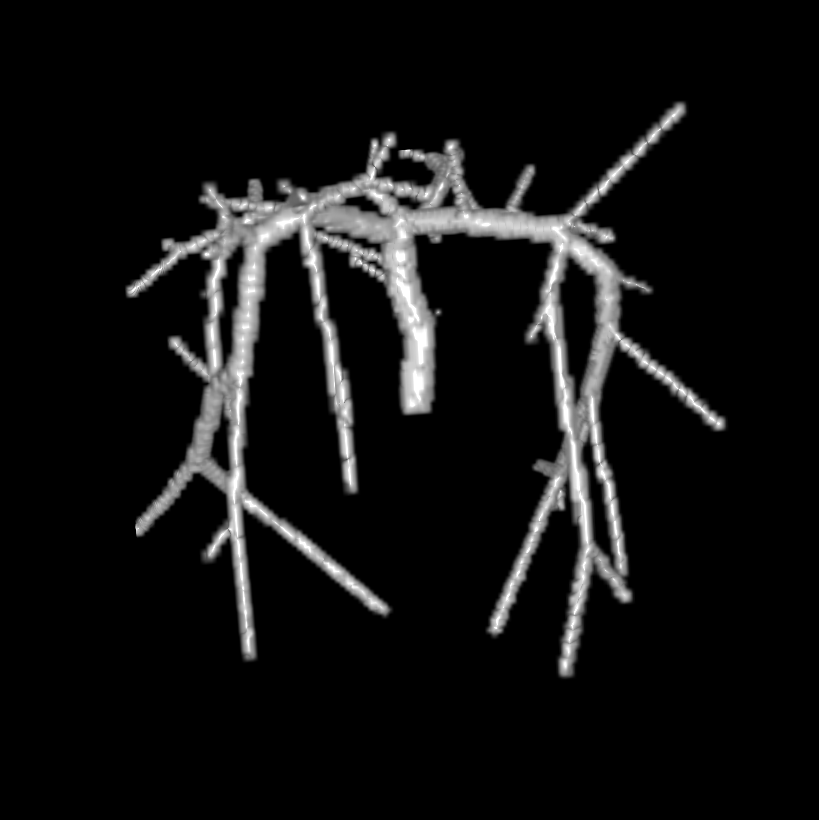
\includegraphics[clip = true, trim = 80 80 80 80, height=3.5cm]{Images/Vascu_4_GT.png}
  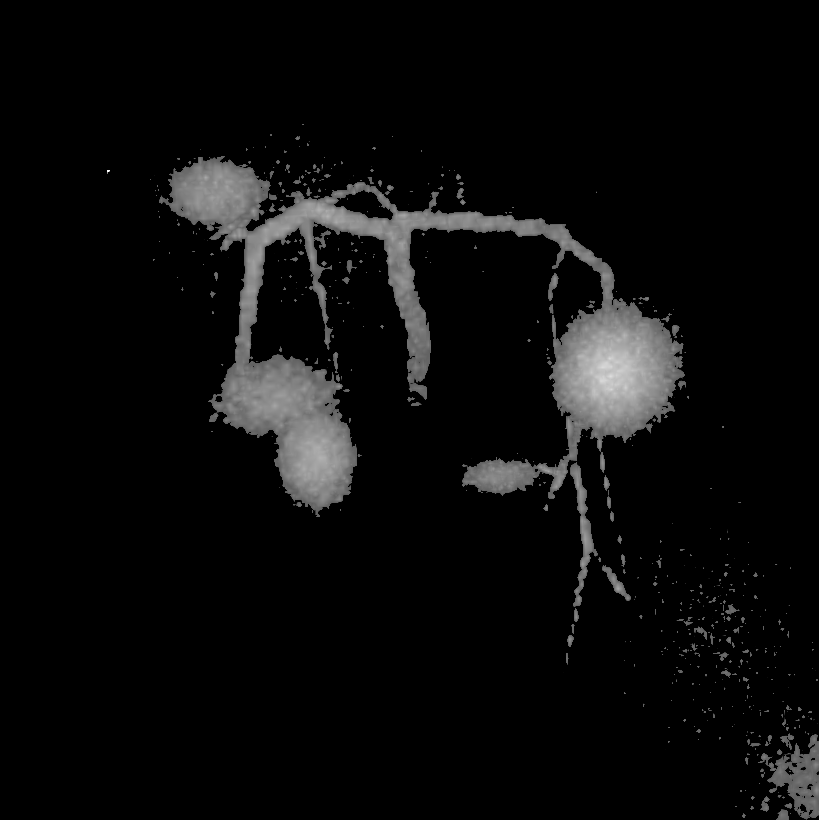
\includegraphics[clip = true, trim = 80 80 80 80, height=3.5cm]{Images/Vascu_4_Baseline.png}
  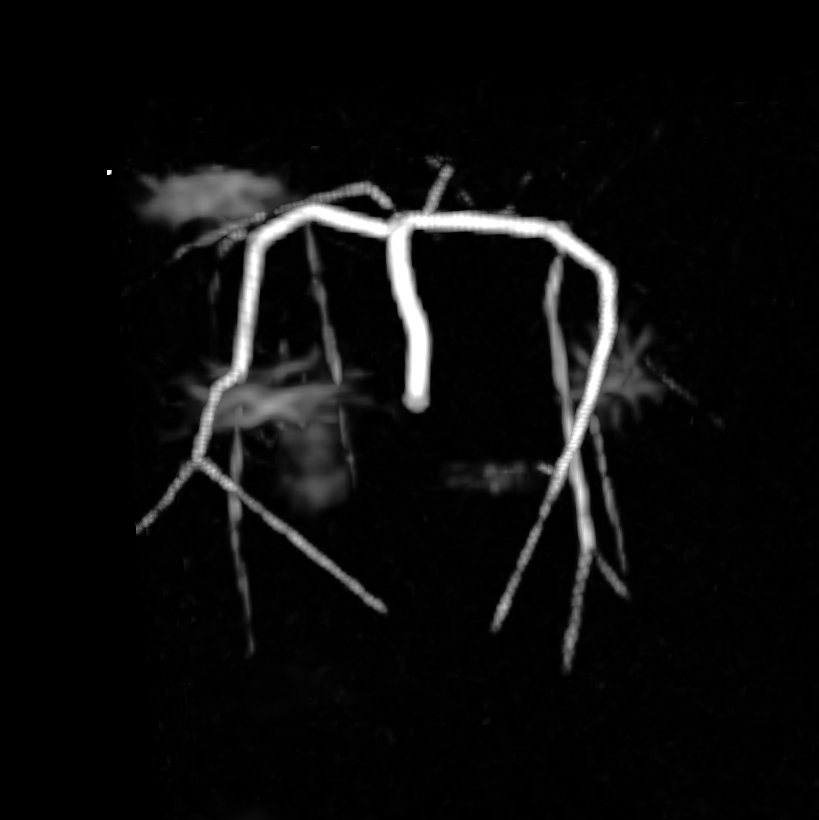
\includegraphics[clip = true, trim = 80 80 80 80, height=3.5cm]{Images/Vascu_4_Frangi.png}
  \\
  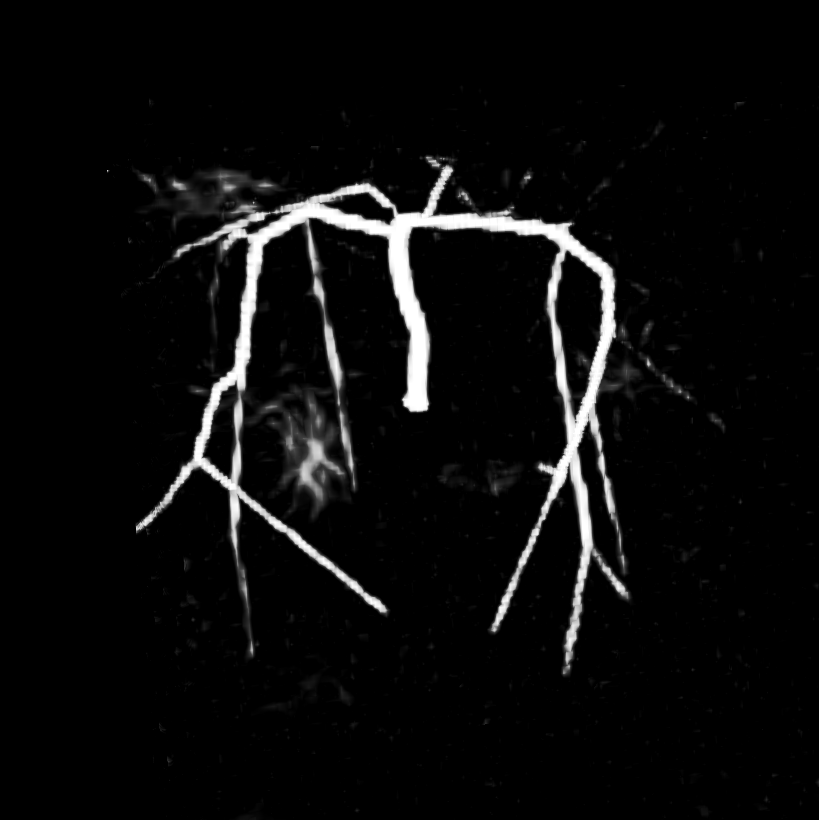
\includegraphics[clip = true, trim = 80 80 80 80, height=3.5cm]{Images/Vascu_4_Jerman.png}
  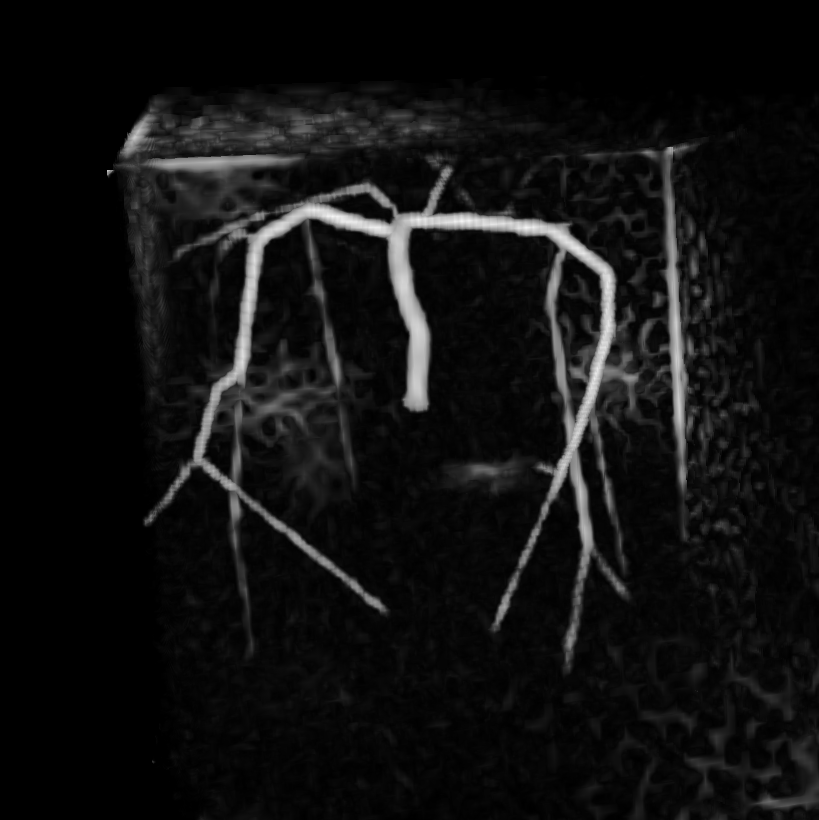
\includegraphics[clip = true, trim = 80 80 80 80, height=3.5cm]{Images/Vascu_4_OOF_GM.png}
  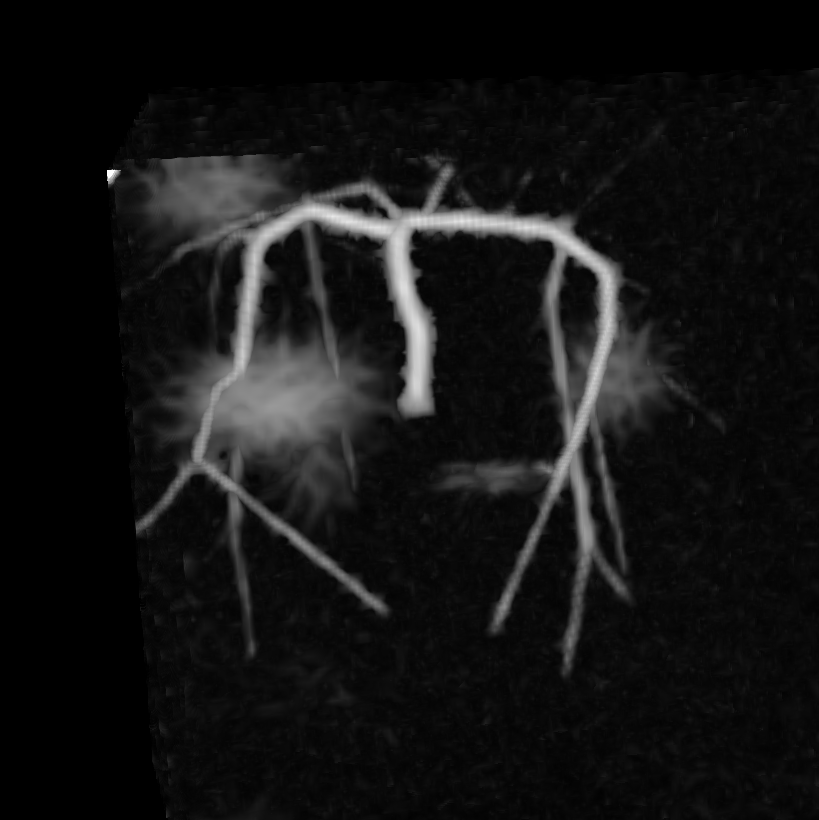
\includegraphics[clip = true, trim = 80 80 80 80, height=3.5cm]{Images/Vascu_4_Meijering.png}
  \\
  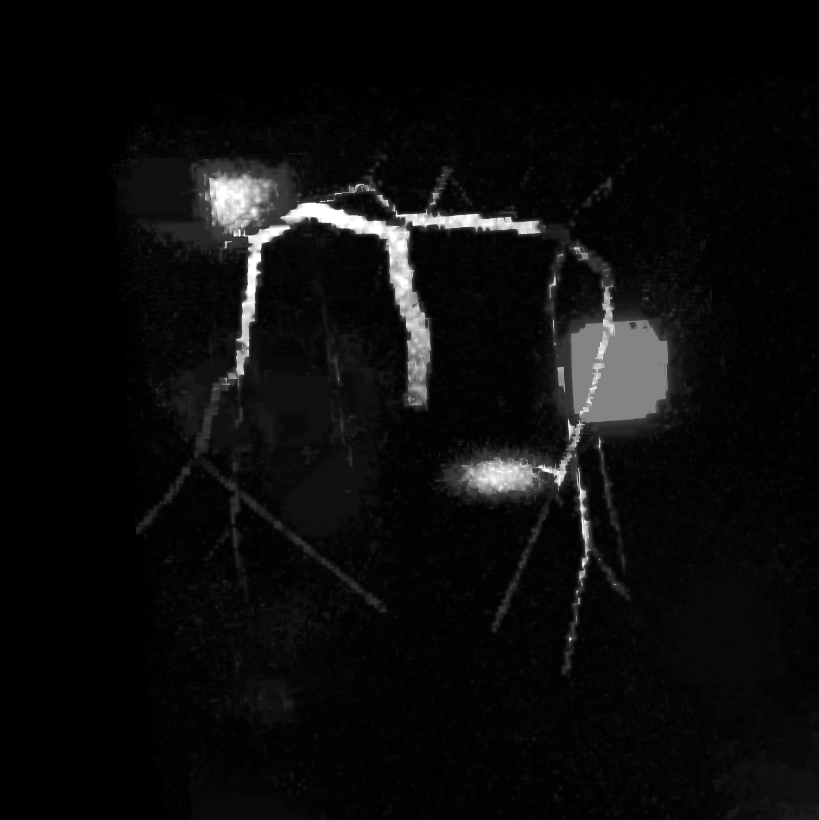
\includegraphics[clip = true, trim = 80 80 80 80, height=3.5cm]{Images/Vascu_4_RORPO.png}
  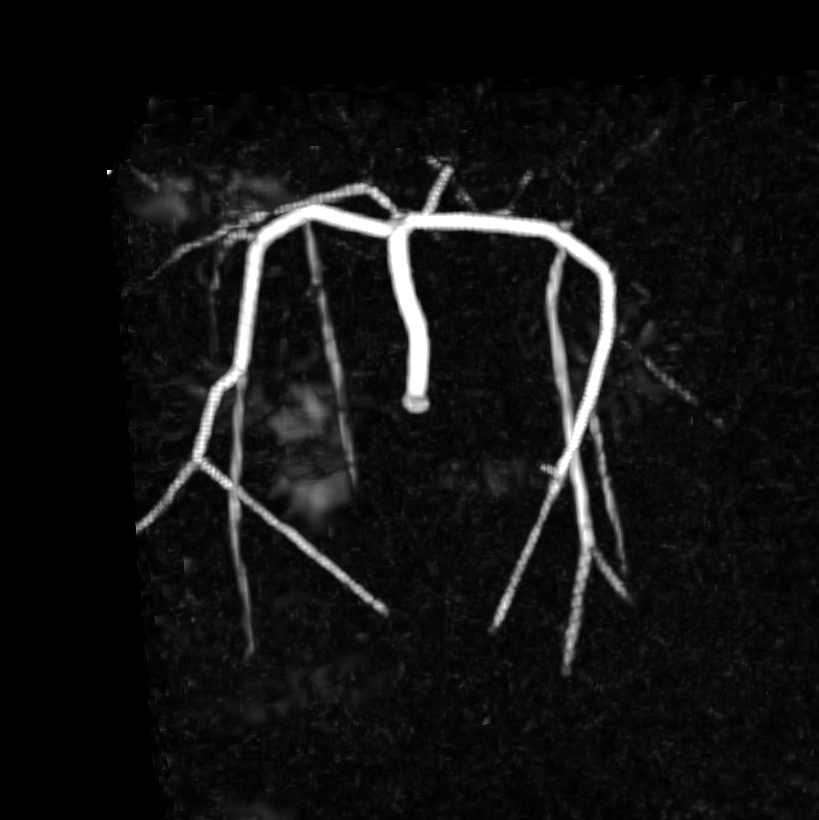
\includegraphics[clip = true, trim = 80 80 80 80, height=3.5cm]{Images/Vascu_4_Sato.png}
  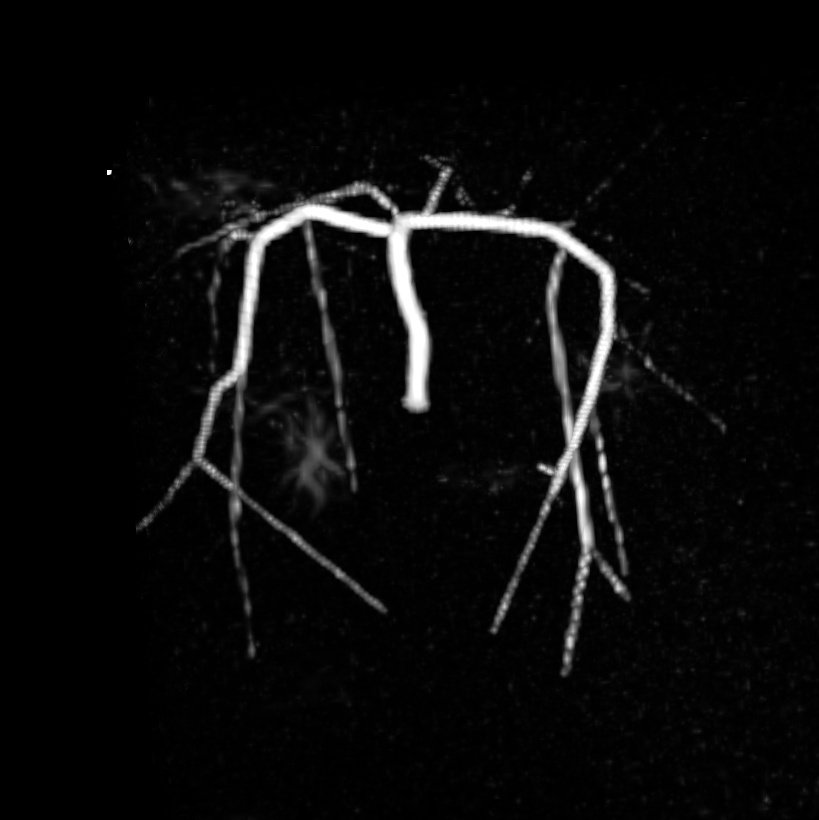
\includegraphics[clip = true, trim = 80 80 80 80, height=3.5cm]{Images/Vascu_4_Zhang.png}

  \caption{Illustration des résultats de filtrage optimisé pour VascuSynth $\sigma=4$.
  Dans l'ordre de lecture vérités terrains, suivies de la référence, Frangi, Jerman, OOF, Meijering, RORPO, Sato et Zhang.}
  \label{fig:qualitative results VascuSynth}
\end{figure}

\subsection{Voisinage des vaisseaux}
Les résultats quantitatifs des sept filtres sont présentés dans les tables \ref{tab:VesselssizeIrcad}--\ref{tab:Vessels size VascuSynth} pour les jeux de données de l'Ircad, Bullitt et VascuSynth.

\paragraph{Ircad}

\begin{table}[H]
  \begin{center}
  \caption{Résultats quantitatifs (moyenne $\pm$ écart-type) par catégorie de tailles de vaisseaux pour l'Ircad.}
  \label{tab:VesselssizeIrcad}
  \resizebox{\textwidth}{!}{    
  \begin{tabular}{lccc|ccc}
                \hline
                & \multicolumn{3}{c}{Voisinage}                                   & \multicolumn{3}{c}{Larges}                                            \\
                \hline
                & MCC  &  Dice & PSNR & MCC  &  Dice  &  PSNR  \\
                Référence	& $ 0.491 \pm	0.118 $ & $	0.527 \pm 0.110 $ & $ 13.110 \pm 1.795 $ & $ 0.552 \pm 	0.130 $ & $	0.597 \pm 0.136 $ & $ 20.938 \pm 2.637 $ \\
                Frangi  	& $ 0.535 \pm	0.073 $ & $	\tbf{0.581} \pm 0.065 $ & $ 19.989 \pm 1.653 $ & $ \tbf{0.580} \pm 	0.072 $ & $	\tbf{0.627} \pm 0.087 $ & $ 22.189 \pm 1.867 $ \\
                Jerman	  & $ 0.501 \pm	0.054 $ & $	0.521 \pm 0.060 $ & $ \tbf{21.464} \pm 1.757 $ & $ 0.480 \pm 	0.065 $ & $	0.496 \pm 0.083 $ & $ \tbf{24.119} \pm 1.972 $ \\
                Meijering	& $ 0.451 \pm	0.061 $ & $	0.522 \pm 0.049 $ & $ 20.091 \pm 1.646 $ & $ 0.545 \pm 	0.055 $ & $	0.669 \pm 0.044 $ & $ 22.407 \pm 1.850 $ \\
                OOF	      & $ 0.498 \pm	0.063 $ & $	0.556 \pm 0.051 $ & $ 19.912 \pm 1.642 $ & $ 0.513 \pm 	0.060 $ & $	0.574 \pm 0.067 $ & $ 22.056 \pm 1.850 $ \\
                RORPO	    & $ 0.491 \pm	0.066 $ & $	0.501 \pm 0.075 $ & $ 20.463 \pm 1.765 $ & $ 0.491 \pm 	0.069 $ & $	0.504 \pm 0.080 $ & $ 22.580 \pm 1.948 $ \\
                Sato	    & $ 0.508 \pm	0.054 $ & $	0.542 \pm 0.057 $ & $ 19.996 \pm 1.679 $ & $ 0.512 \pm 	0.067 $ & $	0.548 \pm 0.086 $ & $ 22.130 \pm 1.861 $ \\
                Zhang	    & $ \tbf{0.535} \pm	0.064 $ & $	0.551 \pm 0.074 $ & $ 20.940 \pm 1.857 $ & $ 0.541 \pm 	0.078 $ & $	0.561 \pm 0.101 $ & $ 23.199 \pm 2.032 $ \\
      
                \hline
                & \multicolumn{3}{c}{Moyens}                                         & \multicolumn{3}{c}{Petits}                                            \\
                \hline
                & MCC  &  Dice & PSNR & MCC  &  Dice  &  PSNR  \\
                Référence	& $ 0.509 \pm 0.121 $ & $	0.557 \pm 0.117 $ & $ 21.250 \pm 2.989 $ & $ 0.391 \pm	0.103 $ & $	0.424 \pm 0.097 $ & $ 18.687 \pm 2.209 $ \\
                Frangi    & $ 0.619 \pm 0.115 $ & $	0.660 \pm 0.113 $ & $ 27.387 \pm 2.554 $ & $ 0.460 \pm	0.123 $ & $	0.506 \pm 0.118 $ & $ 26.624 \pm 2.232 $ \\
                Jerman    & $ 0.604 \pm 0.095 $ & $	0.622 \pm 0.110 $ & $ \tbf{30.111} \pm 3.155 $ & $ 0.502 \pm	0.093 $ & $	0.525 \pm 0.104 $ & $ \tbf{27.991} \pm 2.120 $ \\
                Meijering & $ 0.542 \pm 0.085 $ & $	0.602 \pm 0.082 $ & $ 27.432 \pm 2.474 $ & $ 0.419 \pm	0.088 $ & $	0.462 \pm 0.077 $ & $ 26.723 \pm 2.187 $ \\
                OOF	      & $ \tbf{0.642} \pm 0.097 $ & $	0.681 \pm 0.097 $ & $ 27.334 \pm 2.467 $ & $ \tbf{0.514} \pm	0.103 $ & $	\tbf{0.559} \pm 0.096 $ & $ 26.692 \pm 2.251 $ \\
                RORPO	    & $ 0.547 \pm 0.102 $ & $	0.573 \pm 0.115 $ & $ 28.138 \pm 2.637 $ & $ 0.417 \pm	0.093 $ & $	0.435 \pm 0.104 $ & $ 27.157 \pm 2.354 $ \\
                Sato	    & $ 0.602 \pm 0.096 $ & $	\tbf{0.629} \pm 0.105 $ & $ 27.437 \pm 2.548 $ & $ 0.488 \pm	0.092 $ & $	0.522 \pm 0.091 $ & $ 26.777 \pm 2.277 $ \\
                Zhang	    & $ 0.602 \pm 0.110 $ & $	0.619 \pm 0.126 $ & $ 28.808 \pm 3.119 $ & $ 0.481 \pm	0.110 $ & $	0.497 \pm 0.124 $ & $ 27.471 \pm 2.311 $ \\        
      \hline
      \end{tabular}

  }
  \end{center}
\end{table}


Tous les filtres hessiens et OOF ont des performances qui augmentent significativement quand ils sont calculés dans \maskvessel, puisque les artefacts éloignés des vaisseaux sont ignorés pour ce masque. Dans ce contexte, Frangi et Zhang sont tous les deux les meilleurs filtres (MCC=$0.535$), là où RORPO présentait les meilleurs résultats dans le \maskglobal. En étudiant les performances des filtres en fonction de la taille des vaisseaux rehaussés (\maskvesselLarge,\maskvesselMedium,\maskvesselSmall), on observe que Frangi est capable de bien rehausser les vaisseaux larges (MCC=$0.580$) et moyens (MCC= $0.619$), mais ses performances baissent pour les petits vaisseaux (MCC=$0.460$). À l'inverse, OOF et Jerman rehaussent correctement les petits vaisseaux (MCC=$0.514$ et MCC=$0.502$) mais avec des performances réduites sur les gros vaisseaux (MCC=$0.513$ et MCC=$0.480$).   

\paragraph{Bullitt}

\begin{table}[H]
  \begin{center}
  \label{tab:Vessels size Bullitt}
  \caption{Résultats quantitatifs (moyenne $\pm$ écart-type) par catégorie de tailles de vaisseaux pour Bullitt.}
  
  \begin{tabular}{lccc}
            \hline
            & \multicolumn{3}{c}{Voisinage}                  \\
            \hline
            & MCC & Dice & PSNR  \\
            Baseline	    & $ 0.371 \pm 0.038 $ & $ 0.341 \pm 0.062 $ & $ \tbf{22.291} \pm	0.513 $ \\
            Frangi	      & $ 0.415 \pm 0.028 $ & $ 0.506 \pm 0.026 $ & $ 21.641 \pm	0.517 $ \\
            Jerman	      & $ 0.377 \pm 0.037 $ & $ 0.466 \pm 0.029 $ & $ 21.990 \pm	0.687 $ \\
            Meijering	    & $ 0.288 \pm 0.041 $ & $ 0.412 \pm 0.045 $ & $ 22.076 \pm	0.509 $ \\ 
            OOF	          & $ 0.353 \pm 0.026 $ & $ 0.456 \pm 0.032 $ & $ 21.771 \pm	0.506 $ \\
            RORPO	        & $ \tbf{0.506} \pm 0.022 $ & $ \tbf{0.556} \pm 0.025 $ & $ 21.784 \pm	0.506 $ \\
            Sato	        & $ 0.435 \pm 0.027 $ & $ 0.491 \pm 0.029 $ & $ 21.698 \pm	0.478 $ \\
            Zhang	        & $ 0.348 \pm 0.029 $ & $ 0.460 \pm 0.026 $ & $ 21.430 \pm	0.553 $ \\
      
            \hline
            & \multicolumn{3}{c}{Moyens}                         \\
            \hline    
            & MCC & Dice & PSNR  \\
            Baseline	& $ 0.542 \pm 0.129 $ & $ 0.555 \pm 0.163 $ & $ 33.836 \pm	2.891 $ \\
            Frangi	  & $ 0.605 \pm 0.034 $ & $ 0.684 \pm 0.034 $ & $ 33.262 \pm	2.827 $ \\
            Jerman	  & $ 0.580 \pm 0.048 $ & $ 0.660 \pm 0.055 $ & $ \tbf{34.066} \pm	3.226 $ \\
            Meijering	& $ 0.402 \pm 0.054 $ & $ 0.521 \pm 0.067 $ & $ 34.034 \pm	2.820 $ \\
            OOF	      & $ 0.620 \pm 0.049 $ & $ \tbf{0.690} \pm 0.044 $ & $ 33.621 \pm	2.971 $ \\
            RORPO	    & $ \tbf{0.647} \pm 0.047 $ & $ 0.712 \pm 0.047 $ & $ 33.370 \pm	2.882 $ \\
            Sato	    & $ 0.594 \pm 0.064 $ & $ 0.663 \pm 0.088 $ & $ 33.072 \pm	2.928 $ \\
            Zhang	    & $ 0.577 \pm 0.074 $ & $ 0.655 \pm 0.101 $ & $ 33.789 \pm	2.790 $ \\
            \hline
            & \multicolumn{3}{c}{Petits}                          \\
            \hline
            & MCC & Dice & PSNR  \\
            Baseline	    & $ 0.358 \pm 0.038 $ & $ 0.315 \pm 0.057 $ & $ \tbf{22.771} \pm	0.591 $ \\
            Frangi	      & $ 0.419 \pm 0.024 $ & $ 0.491 \pm 0.026 $ & $ 22.153 \pm	0.609 $ \\
            Jerman  	    & $ 0.376 \pm 0.031 $ & $ 0.445 \pm 0.030 $ & $ 22.352 \pm	0.863 $ \\
            Meijering	    & $ 0.287 \pm 0.040 $ & $ 0.382 \pm 0.044 $ & $ 22.549 \pm	0.593 $ \\
            OOF	          & $ 0.353 \pm 0.025 $ & $ 0.436 \pm 0.038 $ & $ 22.275 \pm	0.586 $ \\
            RORPO	        & $ \tbf{0.510} \pm 0.023 $ & $ \tbf{0.544} \pm 0.027 $ & $ 22.307 \pm	0.590 $ \\
            Sato	        & $ 0.436 \pm 0.024 $ & $ 0.473 \pm 0.031 $ & $ 22.236 \pm	0.572 $ \\
            Zhang	        & $ 0.349 \pm 0.022 $ & $ 0.440 \pm 0.023 $ & $ 21.861 \pm	0.680 $ \\
  \hline
  \end{tabular}
  \end{center}
\end{table}

Localement, les résultats pour \maskglobal et \maskvessel sont similaires puisque le jeu de données ne contient quasiment pas de structures autres que les vaisseaux. Dans ce contexte, RORPO est toujours le meilleur filtre suivi de Sato et Frangi.

\paragraph{VascuSynth}

\begin{table}[H]
  \begin{centering}
  \caption{Résultats quantitatifs (moyenne $\pm$ écart-type) par catégorie de tailles de vaisseaux pour VascuSynth ($\sigma=2$).}
  \label{tab:Vessels size VascuSynth}
  \resizebox{\textwidth}{!}{
  \begin{tabular}{lccc|ccc}
            \hline
            & \multicolumn{3}{c}{Voisinage}  & \multicolumn{3}{c}{Larges}                           \\
            \hline
            & MCC   & Dice & PSNR & MCC & Dice & PSNR  \\
            Baseline	    & $ 0.392 \pm 0.145 $ & $ 0.340 \pm	0.172 $ & $	25.198 \pm	3.109 $ & $ 0.515 \pm 0.293 $ & $ 0.491 \pm 0.307 $ & $ 30.738 \pm 1.278 $ \\
            Frangi	      & $ 0.700 \pm 0.037 $ & $ 0.688 \pm	0.044 $ & $	26.275 \pm	2.814 $ & $ 0.757 \pm 0.022 $ & $ 0.747 \pm 0.025 $ & $ 32.939 \pm 0.934 $ \\
            Jerman	      & $ 0.710 \pm 0.055 $ & $ 0.702 \pm	0.067 $ & $	\tbf{29.880} \pm	3.007 $ & $ 0.735 \pm 0.027 $ & $ 0.722 \pm 0.031 $ & $ 36.312 \pm 0.973 $ \\
            Meijering	    & $ \tbf{0.725} \pm 0.034 $ & $ \tbf{0.753} \pm	0.035 $ & $	27.305 \pm	2.969 $ & $ \tbf{0.818} \pm 0.028 $ & $ \tbf{0.834} \pm 0.028 $ & $ 34.217 \pm 0.978 $ \\
            OOF	          & $ 0.648 \pm 0.043 $ & $ 0.624 \pm	0.053 $ & $	28.275 \pm	2.968 $ & $ 0.714 \pm 0.025 $ & $ 0.696 \pm 0.029 $ & $ 35.068 \pm 0.980 $ \\
            RORPO	        & $ 0.639 \pm 0.082 $ & $ 0.619 \pm	0.096 $ & $	29.406 \pm	3.407 $ & $ 0.713 \pm 0.165 $ & $ 0.694 \pm 0.197 $ & $ \tbf{37.049} \pm 1.574 $ \\
            Sato	        & $ 0.661 \pm 0.034 $ & $ 0.642 \pm	0.042 $ & $	26.938 \pm	2.867 $ & $ 0.731 \pm 0.024 $ & $ 0.719 \pm 0.028 $ & $ 33.699 \pm 0.945 $ \\
            Zhang	        & $ 0.624 \pm 0.042 $ & $ 0.594 \pm	0.053 $ & $	26.225 \pm	2.809 $ & $ 0.713 \pm 0.041 $ & $ 0.696 \pm 0.050 $ & $ 32.893 \pm 0.936 $ \\
      
            \hline
            & \multicolumn{3}{c}{Moyens}                         & \multicolumn{3}{c}{Petits}                           \\
            \hline
            & MCC  & Dice & PSNR & MCC & Dice & PSNR  \\
            Baseline	    & $ 0.415 \pm 0.176 $ & $ 0.355 \pm 0.202 $ & $	26.699 \pm 1.974 $ & $	0.284 \pm 0.125 $ & $ 0.218 \pm 0.129 $ & $ 27.954 \pm 3.858 $ \\
            Frangi	      & $ 0.715 \pm 0.035 $ & $ 0.698 \pm 0.041 $ & $	28.986 \pm 2.026 $ & $	0.683 \pm 0.056 $ & $ 0.657 \pm 0.069 $ & $ 30.328 \pm 3.627 $ \\
            Jerman	      & $ 0.708 \pm 0.047 $ & $ 0.691 \pm 0.057 $ & $	\tbf{32.360} \pm 2.236 $ & $	\tbf{0.730} \pm 0.073 $ & $ \tbf{0.719} \pm 0.090 $ & $ \tbf{34.315} \pm 4.028 $ \\
            OOF	          & $ \tbf{0.768} \pm 0.031 $ & $ \tbf{0.785} \pm 0.031 $ & $	30.159 \pm 2.141 $ & $	0.660 \pm 0.072 $ & $ 0.652 \pm 0.086 $ & $ 31.054 \pm 3.723 $ \\
            Meijering	    & $ 0.672 \pm 0.040 $ & $ 0.646 \pm 0.049 $ & $	31.016 \pm 2.152 $ & $	0.615 \pm 0.071 $ & $ 0.572 \pm 0.091 $ & $ 32.202 \pm 3.802 $ \\
            RORPO	        & $ 0.670 \pm 0.087 $ & $ 0.647 \pm 0.101 $ & $	32.281 \pm 2.506 $ & $	0.566 \pm 0.108 $ & $ 0.523 \pm 0.118 $ & $ 32.660 \pm 3.946 $ \\
            Sato	        & $ 0.675 \pm 0.035 $ & $ 0.649 \pm 0.042 $ & $	29.659 \pm 2.078 $ & $	0.647 \pm 0.047 $ & $ 0.615 \pm 0.059 $ & $ 30.939 \pm 3.674 $ \\
            Zhang	        & $ 0.648 \pm 0.044 $ & $ 0.616 \pm 0.054 $ & $	28.936 \pm 2.024 $ & $	0.580 \pm 0.054 $ & $ 0.528 \pm 0.071 $ & $ 30.278 \pm 3.618 $ \\
  \hline
  \end{tabular}
  }
  \end{centering} 
\end{table}

Globalement, le rehaussement des vaisseaux est le mieux réalisé par Frangi, à l'exception du plus faible niveau de bruit où Meijering obtient les meilleurs résultats. Une analyse plus fine des résultats par tailles montre que Meijering et Jerman obtiennent de meilleurs résultats que Frangi sur les vaisseaux moyens et petits pour de faibles niveaux de bruit.  Dans les autres cas, Frangi produit de meilleurs résultats pour \maskvessel.

\subsection{Bifurcations}

\todo{Est-ce que le tableau du Dice pour les bifurcations et une discussion quantitative est nécessaire ? On ne l'a pas fait dans des précédents travaux, mais j'ai le sentiment que c'est nécessaire pour cette partie...}

\begin{figure}[H]
  \centering
      \begin{subfigure}[t]{0.30\textwidth}
        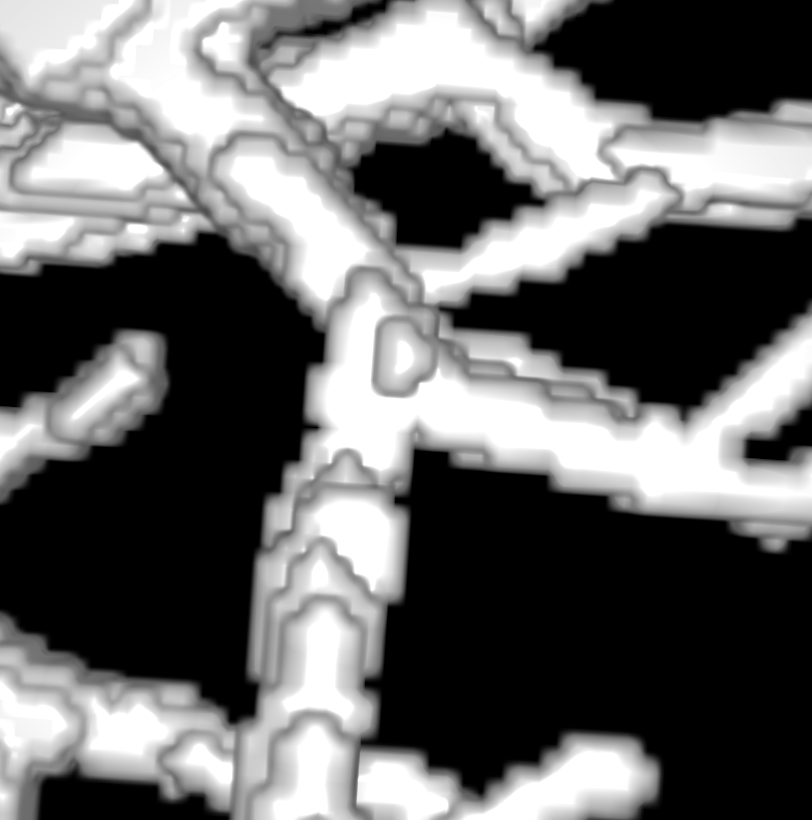
\includegraphics[clip = true, trim  = 0 50 0 80, width=30mm]{Images/Ircad_k_GT.png}
        \caption{Vérité terrain}
      \end{subfigure}
      \begin{subfigure}[t]{0.30\textwidth}
        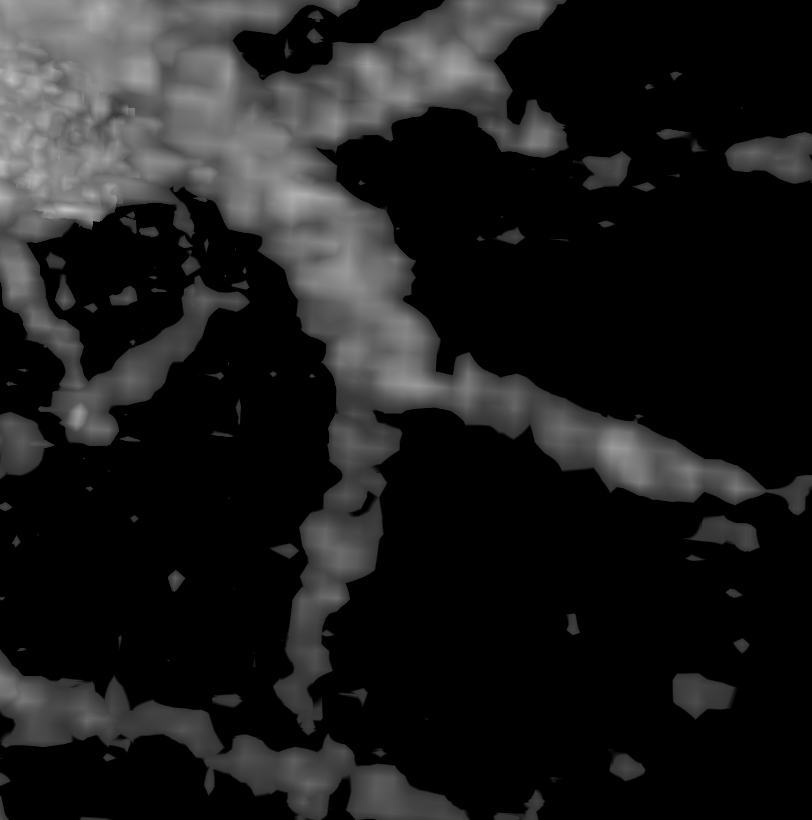
\includegraphics[clip = true, trim  = 0 50 0 80, width=30mm]{Images/Ircad_k_Baseline.png}
        \caption{Référence}
      \end{subfigure}
      \begin{subfigure}[t]{0.30\textwidth}
        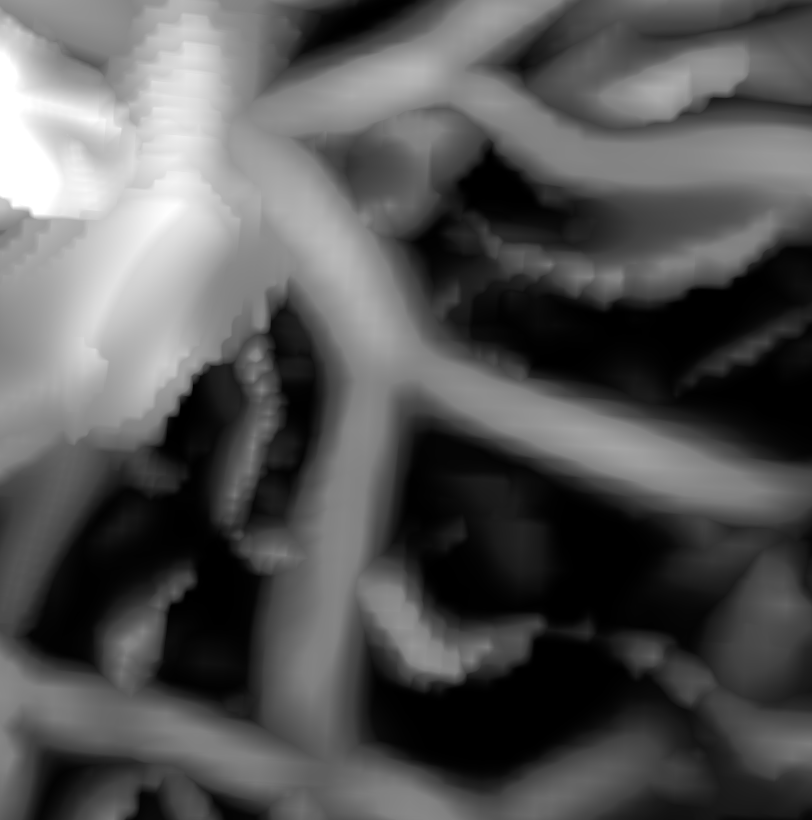
\includegraphics[clip = true, trim  = 0 50 0 80, width=30mm]{Images/Ircad_k_Frangi.png}
        \caption{Frangi}
      \end{subfigure}
      \begin{subfigure}[t]{0.30\textwidth}
        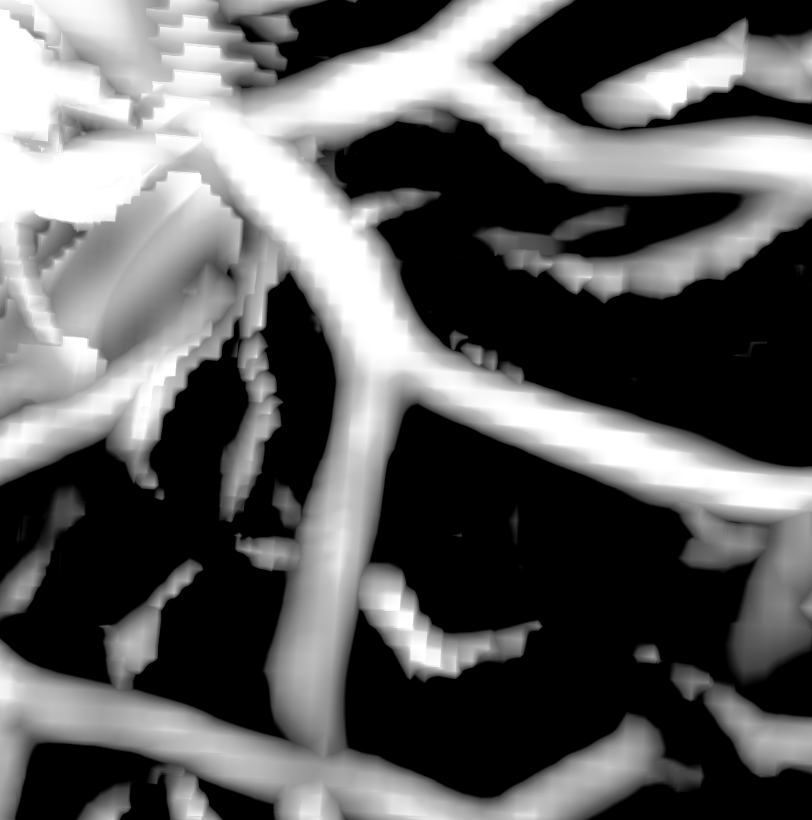
\includegraphics[clip = true, trim  = 0 50 0 80, width=30mm]{Images/Ircad_k_Jerman.png}
        \caption{Jerman}
      \end{subfigure}
      \begin{subfigure}[t]{0.30\textwidth}
        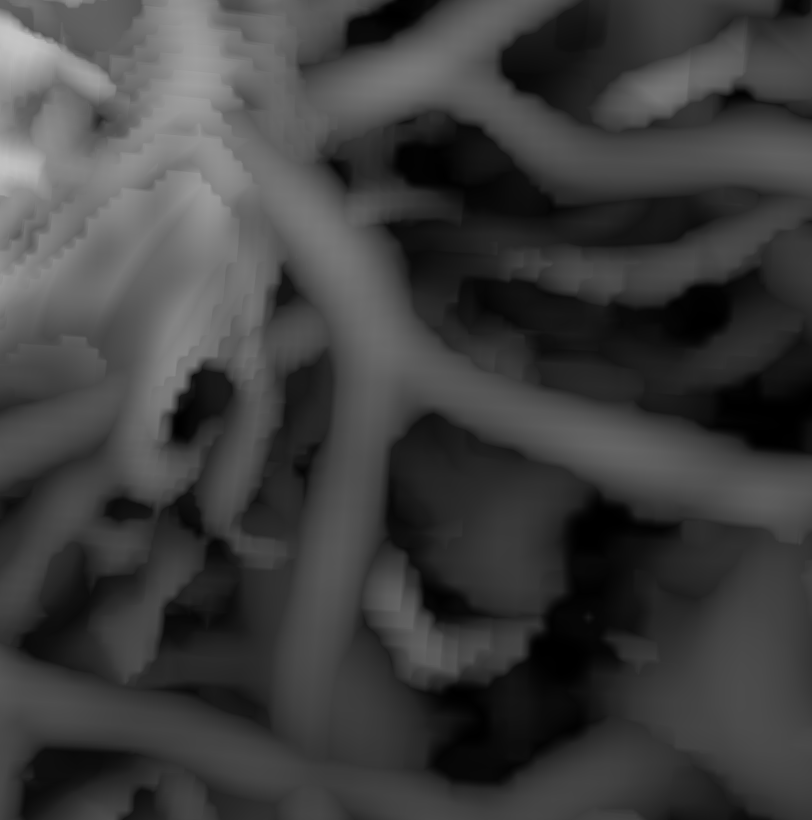
\includegraphics[clip = true, trim  = 0 50 0 80, width=30mm]{Images/Ircad_k_OOF_GM.png}
        \caption{OOF}
      \end{subfigure}
      \begin{subfigure}[t]{0.30\textwidth}
        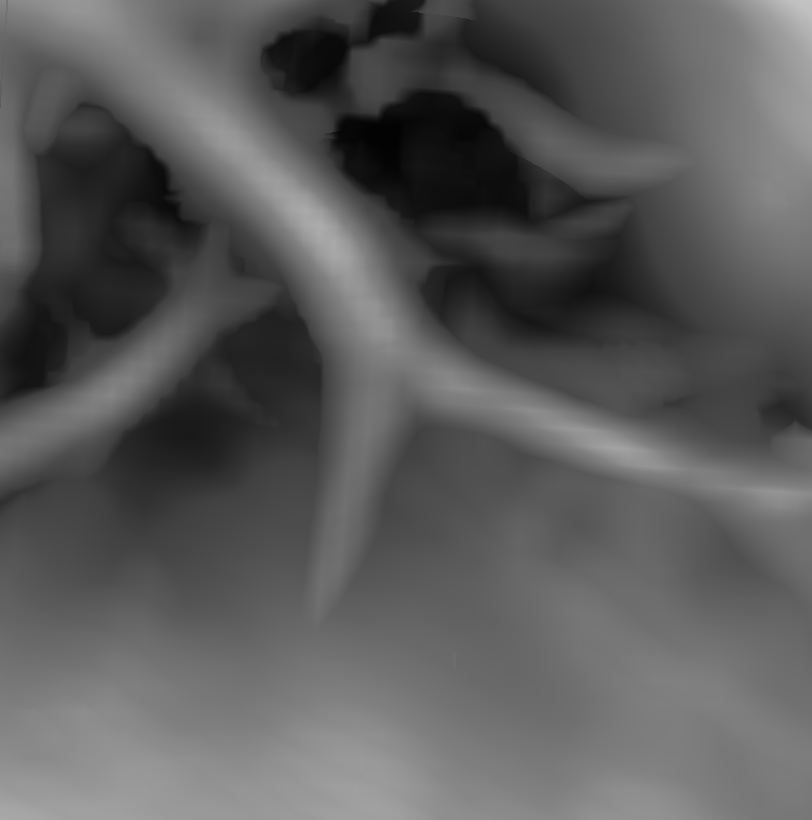
\includegraphics[clip = true, trim  = 0 50 0 80, width=30mm]{Images/Ircad_k_Meijering.png}
        \caption{Meijering}
      \end{subfigure}
      \begin{subfigure}[t]{0.30\textwidth}
        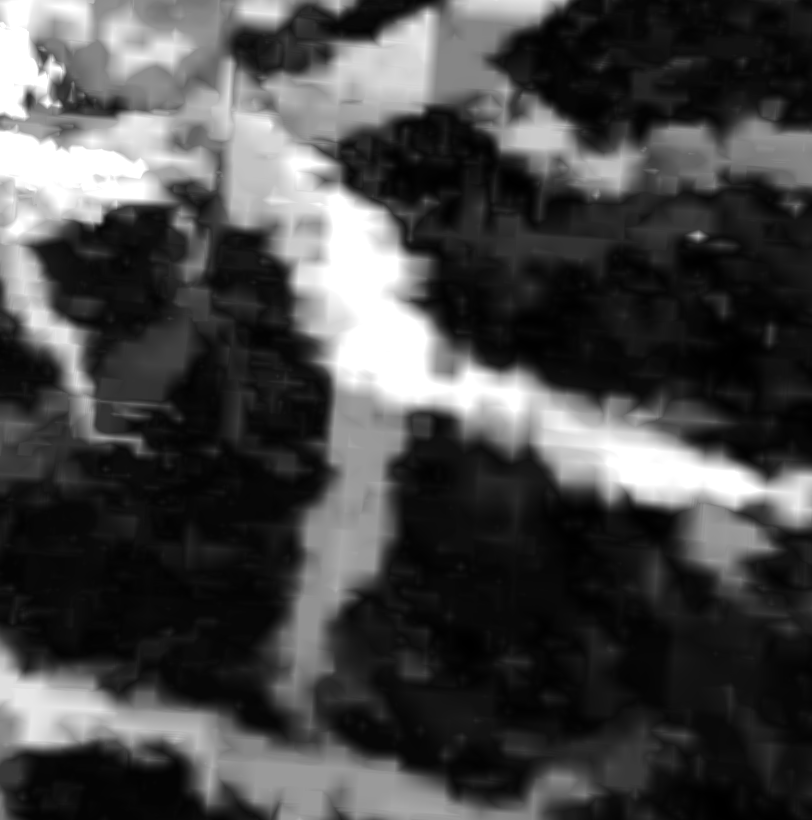
\includegraphics[clip = true, trim  = 0 50 0 80, width=30mm]{Images/Ircad_k_RORPO.png}
        \caption{RORPO}
      \end{subfigure}
      \begin{subfigure}[t]{0.30\textwidth}
        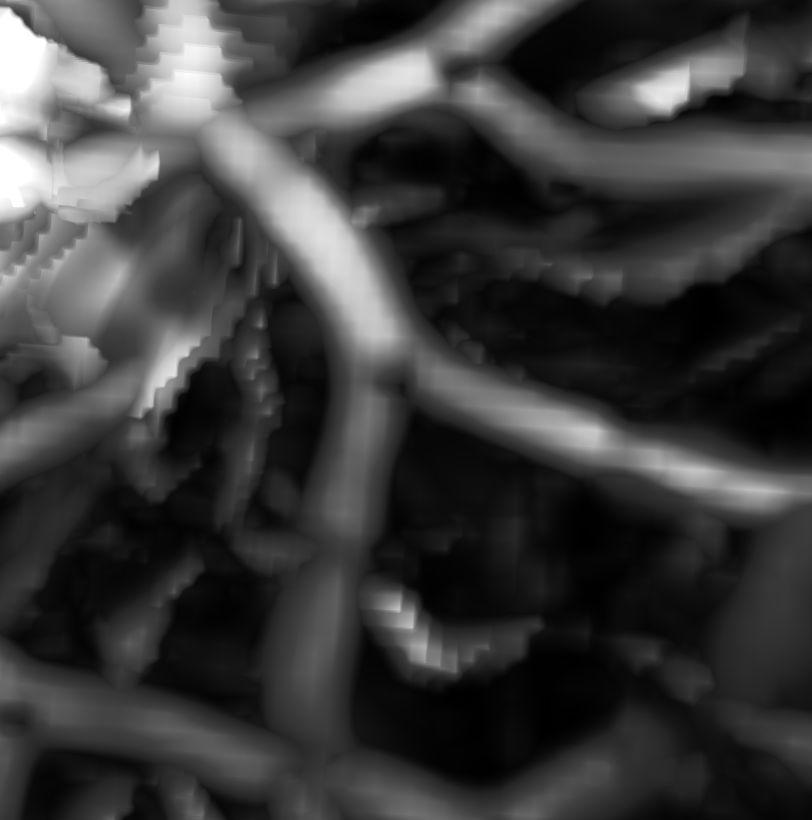
\includegraphics[clip = true, trim  = 0 50 0 80, width=30mm]{Images/Ircad_k_Sato.png}
        \caption{Sato}
      \end{subfigure}
      \begin{subfigure}[t]{0.30\textwidth}
        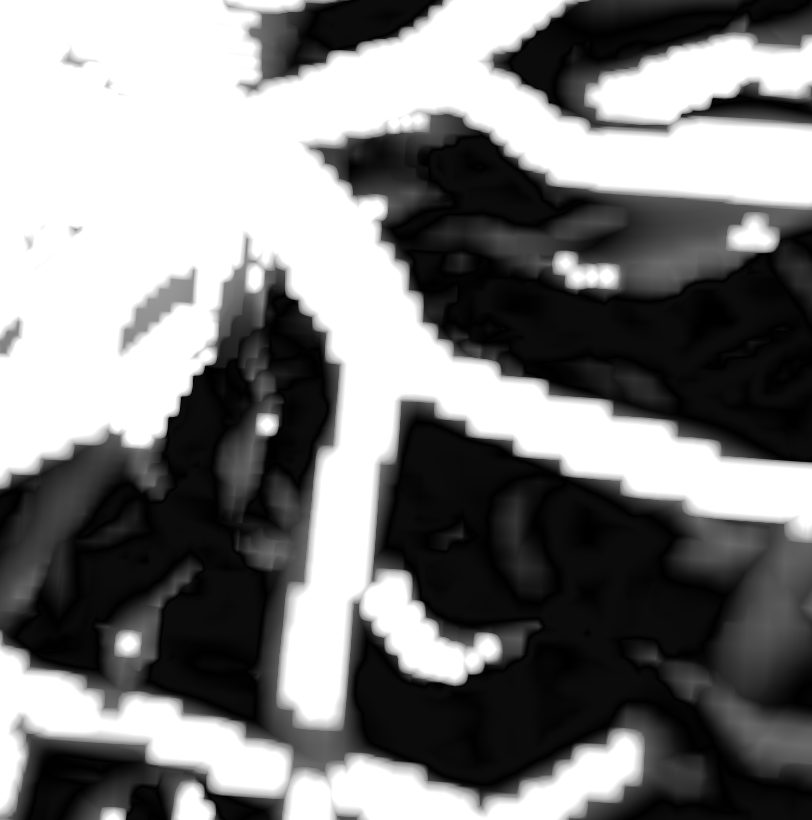
\includegraphics[clip = true, trim  = 0 50 0 80, width=30mm]{Images/Ircad_k_Zhang.png}
        \caption{Zhang}
      \end{subfigure}

      \caption{MIP des filtres avec les meilleurs paramètres sur une bifurcation pour le jeu de données de l'Ircad. La référence est l'image originale masquée et seuillée de manière optimale par rapport au MCC.
      }
      \label{fig:bifurcation_Ircad}
  \end{figure}
  
  \begin{figure}[H]
    \centering
    \begin{subfigure}[t]{0.24\textwidth}
      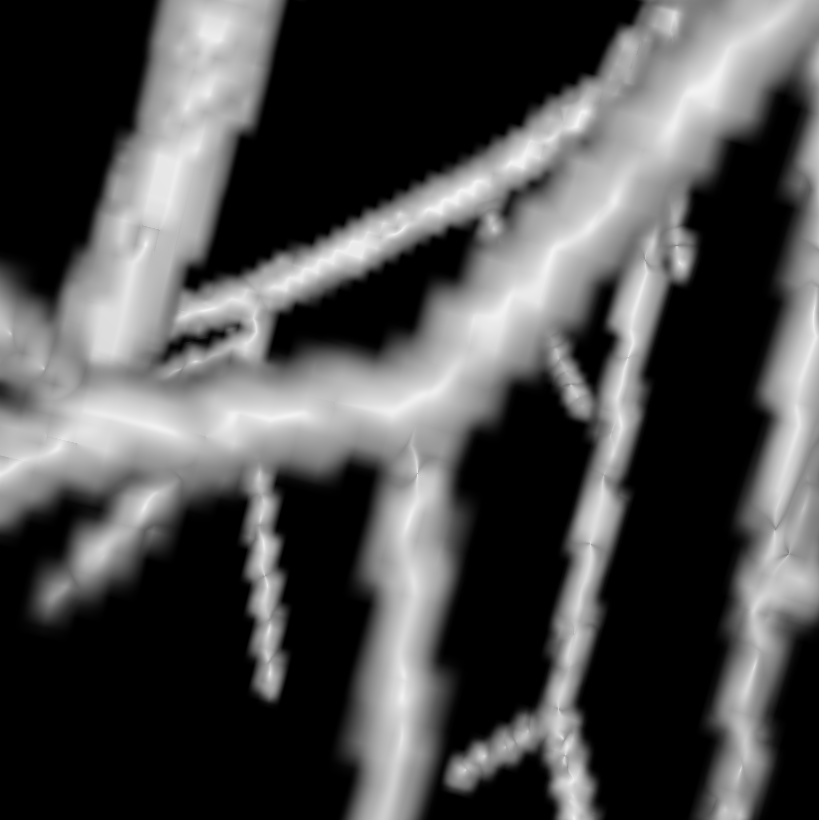
\includegraphics[clip = true, trim  =  170 230 150 240, width=30mm]{Images/Vascu_2_k_GT.png}
      \caption{Vérité terrain}
    \end{subfigure}
    \begin{subfigure}[t]{0.24\textwidth}
      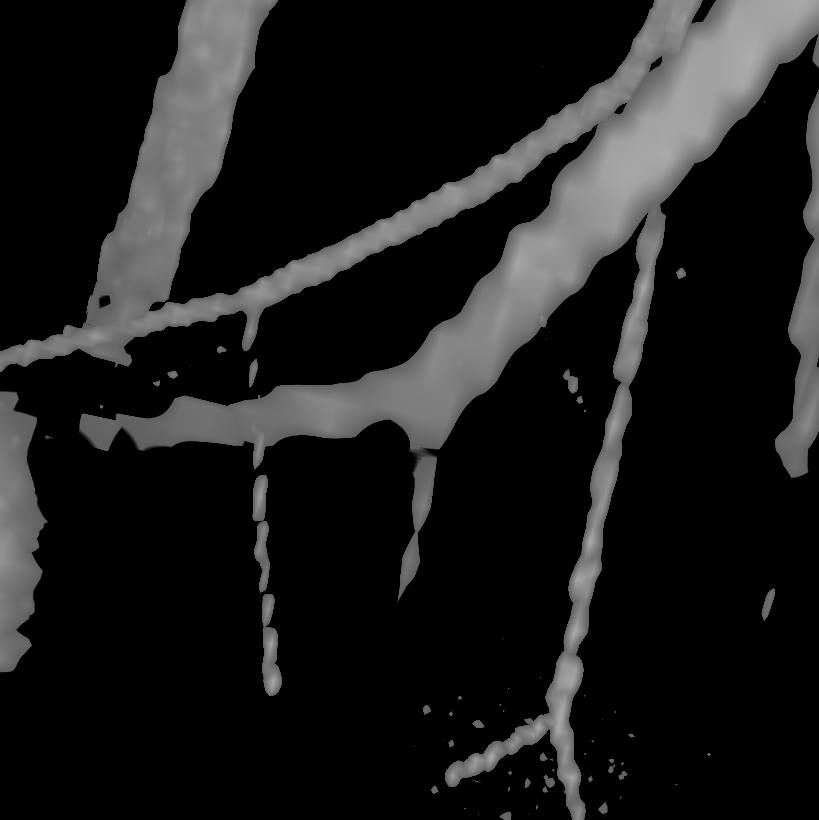
\includegraphics[clip = true, trim  =  170 230 150 240, width=30mm]{Images/Vascu_2_k_Baseline.png}
      \caption{Référence}
    \end{subfigure}
    \begin{subfigure}[t]{0.24\textwidth}
      \includegraphics[clip = true, trim  =  170 230 150 240, width=30mm]{Images/Vascu_2_k_Frangi.png}
      \caption{Frangi}
    \end{subfigure}
    \begin{subfigure}[t]{0.24\textwidth}
      \includegraphics[clip = true, trim  =  170 230 150 240, width=30mm]{Images/Vascu_2_k_Jerman.png}
      \caption{Jerman}
    \end{subfigure}
    \begin{subfigure}[t]{0.24\textwidth}
      \includegraphics[clip = true, trim  =  170 230 150 240, width=30mm]{Images/Vascu_2_k_OOF_GM.png}
      \caption{OOF}
    \end{subfigure}
    \begin{subfigure}[t]{0.24\textwidth}
      \includegraphics[clip = true,trim  =  170 230 150 240, width=30mm]{Images/Vascu_2_k_Meijering.png}
      \caption{Meijering}
    \end{subfigure}
    \begin{subfigure}[t]{0.24\textwidth}
      \includegraphics[clip = true, trim  =  170 230 150 240, width=30mm]{Images/Vascu_2_k_RORPO.png}
      \caption{RORPO}
    \end{subfigure}
    \begin{subfigure}[t]{0.24\textwidth}
      \includegraphics[clip = true, trim  =  170 230 150 240, width=30mm]{Images/Vascu_2_k_Sato.png}
      \caption{Sato}
    \end{subfigure}
    \begin{subfigure}[t]{0.24\textwidth}
      \includegraphics[clip = true, trim  =  170 230 150 240, width=30mm]{Images/Vascu_2_k_Zhang.png}
      \caption{Zhang}
    \end{subfigure}

        \caption{MIP des filtres avec les meilleurs paramètres sur une bifurcation pour le jeu de données VascuSynth avec $\sigma=2$. La référence est l'image originale masquée et seuillée de manière optimale par rapport au MCC.
        }
      \label{fig:bifurcation_vascu}
  \end{figure}


\begin{figure}[H]
  \centering
      \begin{subfigure}[t]{0.33\textwidth}
          \begin{tikzpicture}
              \node[anchor=south west,inner sep=0] (image) at (0,0) {\includegraphics[clip = true, trim = 40 100 40 70, width=4cm]{Images/Bullitt_k_GT.png}};
              \begin{scope}[x={(image.south east)},y={(image.north west)}]
                  \draw[green,thick] (0.33,0.60) rectangle (0.43,0.75);
                  \draw[red,thick] (0.50,0.10) rectangle (0.65,0.35);
              \end{scope}
          \end{tikzpicture}
          \caption{Vérité terrain}
        \end{subfigure}
      \begin{subfigure}[t]{0.33\textwidth}
          \begin{tikzpicture}
              \node[anchor=south west,inner sep=0] (image) at (0,0) {\includegraphics[clip = true, trim = 40 100 40 70,  width=4cm]{Images/Bullitt_k_Baseline.png}};
              \begin{scope}[x={(image.south east)},y={(image.north west)}]
                  \draw[green,thick] (0.33,0.60) rectangle (0.43,0.75);
                  \draw[red,thick] (0.50,0.10) rectangle (0.65,0.35);
              \end{scope}
          \end{tikzpicture}
          \caption{Référence}
        \end{subfigure}
      \begin{subfigure}[t]{0.33\textwidth}
          \begin{tikzpicture}
                  \node[anchor=south west,inner sep=0] (image) at (0,0) {\includegraphics[clip = true, trim = 40 100 40 70,  width=4cm]{Images/Bullitt_k_Frangi.png}};
              \begin{scope}[x={(image.south east)},y={(image.north west)}]
                  \draw[green,thick] (0.33,0.60) rectangle (0.43,0.75);
                  \draw[red,thick] (0.50,0.10) rectangle (0.65,0.35);
              \end{scope}
          \end{tikzpicture}
          \caption{Frangi}
        \end{subfigure}
      \begin{subfigure}[t]{0.33\textwidth}
          \begin{tikzpicture}
                  \node[anchor=south west,inner sep=0] (image) at (0,0) {\includegraphics[clip = true, trim = 40 100 40 70,  width=4cm]{Images/Bullitt_k_Jerman.png}};
              \begin{scope}[x={(image.south east)},y={(image.north west)}]
                  \draw[green,thick] (0.33,0.60) rectangle (0.43,0.75);
                  \draw[red,thick] (0.50,0.10) rectangle (0.65,0.35);
              \end{scope}
          \end{tikzpicture}
          \caption{Jerman}
        \end{subfigure}

      \begin{subfigure}[t]{0.33\textwidth}
          \begin{tikzpicture}
                  \node[anchor=south west,inner sep=0] (image) at (0,0) {\includegraphics[clip = true, trim = 40 100 40 70,  width=4cm]{Images/Bullitt_k_OOF_GM.png}};
              \begin{scope}[x={(image.south east)},y={(image.north west)}]
                  \draw[green,thick] (0.33,0.60) rectangle (0.43,0.75);
                  \draw[red,thick] (0.50,0.10) rectangle (0.65,0.35);
              \end{scope}
          \end{tikzpicture}
          \caption{OOF}
        \end{subfigure}
      \begin{subfigure}[t]{0.33\textwidth}
          \begin{tikzpicture}
                  \node[anchor=south west,inner sep=0] (image) at (0,0) {\includegraphics[clip = true, trim = 40 100 40 70,  width=4cm]{Images/Bullitt_k_Meijering.png}};
              \begin{scope}[x={(image.south east)},y={(image.north west)}]
                  \draw[green,thick] (0.33,0.60) rectangle (0.43,0.75);
                  \draw[red,thick] (0.50,0.10) rectangle (0.65,0.35);
              \end{scope}
          \end{tikzpicture}
          \caption{Meijering}
      \end{subfigure}
      \begin{subfigure}[t]{0.33\textwidth}
          \begin{tikzpicture}
                  \node[anchor=south west,inner sep=0] (image) at (0,0) {\includegraphics[clip = true, trim = 40 100 40 70,  width=4cm]{Images/Bullitt_k_RORPO.png}};
              \begin{scope}[x={(image.south east)},y={(image.north west)}]
                  \draw[green,thick] (0.33,0.60) rectangle (0.43,0.75);
                  \draw[red,thick] (0.50,0.10) rectangle (0.65,0.35);
              \end{scope}
          \end{tikzpicture}
          \caption{RORPO}
        \end{subfigure}
      \begin{subfigure}[t]{0.33\textwidth}
          \begin{tikzpicture}
                  \node[anchor=south west,inner sep=0] (image) at (0,0) {\includegraphics[clip = true, trim = 40 100 40 70,  width=4cm]{Images/Bullitt_k_Sato.png}};
              \begin{scope}[x={(image.south east)},y={(image.north west)}]
                  \draw[green,thick] (0.33,0.60) rectangle (0.43,0.75);
                  \draw[red,thick] (0.50,0.10) rectangle (0.65,0.35);
              \end{scope}
          \end{tikzpicture}
          \caption{Sato}
        \end{subfigure}
      \begin{subfigure}[t]{0.33\textwidth}
          \begin{tikzpicture}
                  \node[anchor=south west,inner sep=0] (image) at (0,0) {\includegraphics[clip = true, trim = 40 100 40 70,  width=4cm]{Images/Bullitt_k_Zhang.png}};
              \begin{scope}[x={(image.south east)},y={(image.north west)}]
                  \draw[green,thick] (0.33,0.60) rectangle (0.43,0.75);
                  \draw[red,thick] (0.50,0.10) rectangle (0.65,0.35);
              \end{scope}
          \end{tikzpicture}
          \caption{Zhang}
        \end{subfigure}
      
        \caption{
        MIP des vaisseaux au centre du cerveau pour le jeu de données Bullitt. Ces vaisseaux sont situés sur le même plan, illustrant ainsi les vaisseaux proches (rouge) et les bifurcations (vert).}
      \label{fig:bifurcation_Bullitt}
\end{figure}

Le filtrage des bifurcations est présenté visuellement dans les figures \ref{fig:bifurcation_Ircad} et \ref{fig:bifurcation_vascu} pour VascuSynth et l'Ircad, tandis que les bifurcations et les vaisseaux adjacents de Bullitt sont présentés dans les figures \ref{fig:bifurcation_Bullitt}.

Qualitativement, nous observons que les filtres de Frangi et Sato présentent une perte de signal au centre des bifurcations pour l'Ircad et Bullitt et sur les pourtours de la bifurcation pour VascuSynth. Cette perte de signal n'a pas été observée pour les autres filtres. Le déplacement de la perte de signal s'éloignant des bords pour VascunSynth peuvent s'expliquer par une géométrie particulière pour ce jeu de données. En effet, les nouvelles branches partant d'un vaisseau principal, plus gros, ont une épaisseur plus réduite. Le centre de la bifurcation se retrouve translaté de l'intersection des deux vaisseaux à la base du plus petit. Concernant les vaisseaux adjacents, certains filtres ont une tendance à fusionner les vaisseaux très proches. Ces filtres sont Jerman, Meijering et Zhang. Les autres filtres tels que Frangi, Sato, OOF et RORPO semblent plus robustes à cet effet. En particulier, cette robustesse est assurée par la propriété d'anti-extensivité pour RORPO.

\section{Discussion}

En se basant sur ces résultats d'expériences, il est possible de formuler quelques recommandations en fonction du masque de région d'intérêt.

Nous avons observé que les performances de Meijering sont faibles sur les jeux de données réels, car le filtre rehausse fortement le bruit. Ce comportement est consistant avec le fait que Meijering est un filtre dédié au rehaussement dans des images très faiblement contrastés pour des applications de tracking. Il faut toutefois noter que Meijering présente de bons résultats sur les données synthétiques de VascuSynth. Il peut être intéressant d’appliquer ce Meijering dans plusieurs contextes :

\begin{itemize}
  \item Les images sont faiblement contrastées et présentent une géométrie des vaisseaux relativement droite sans variations de diamètres.
  \item L'utilisateur choisit d'appliquer une segmentation basée sur une stratégie de tracking et/ou applique une stratégie de post-traitement capable d'identifier les faux positifs.
\end{itemize}

OOF, couplé avec la mesure de tubularité de la moyenne géométrique, présente des résultats relativement faibles sur les jeux de données, ce qui peut s'expliquer par deux éléments : (1) le choix de la mesure dont le pouvoir de discrimination entre les plateaux et les structures tubulaires est faible; et (2) OOF est basé sur l'hypothèse de coupes des vaisseaux à géométrie circulaire, ce qui en pratique n'est pas toujours le cas, en particulier pour l'Ircad. Il convient aussi de noter que OOF est un cadre d'espace d'échelles et que différentes mesures de tubularité peuvent être utilisées en fonction de l'application d'intérêt. OOF est un bon choix dans les cas suivants : 

\begin{itemize}
  \item Les vaisseaux présentent des coupes circulaires.
  \item Les réseaux vasculaires présentent un nombre important de vaisseaux adjacents.
\end{itemize}

Sato et Frangi présentent tous les deux de bonnes performances dans notre banc de test. Ces deux filtres proposent un bon compromis entre sensibilité et spécificité, mais produisent la plupart du temps une perte de signal au niveau des bifurcations. Nous recommandons Frangi dans les cas suivants :

\begin{itemize}
  \item Les vaisseaux dans les images sont de tailles supérieures à quelques voxels.
  \item L'utilisateur a besoin d'un contrôle efficace sur le niveau de bruit à filtrer, au prix de la perte des petits vaisseaux.
\end{itemize}

Sato est recommandé dans les cas suivants :

\begin{itemize}
  \item Les images présentent peu de bruit.
  \item Les vaisseaux ont des coupes circulaires.
  \item Les réseaux vasculaires comportent des vaisseaux adjacents.
\end{itemize}

Jerman présente de bonnes performances avec une sensibilité importante et rehausse nettement les contours de vaisseaux. Cependant, le filtre a tendance à être plus sensible au bruit que les filtres hessiens classiques (i.e. Frangi et Sato) et partage la même tendance à surestimer le volume des vaisseaux. Nous recommandons le filtre de Jerman dans les cas suivants : 

\begin{itemize}
\item Les images avec de petits vaisseaux.
\item Les images avec un faible niveau de bruit.
\end{itemize} 

Zhang est une version modifiée de Jerman, créé pour être moins sensible aux bords et aux artefacts de bordure. Malheureusement la méthode est limitée à des organes spécifiques (ici le  foie). Bien que la méthode propose des résultats intéressants, celle-ci requiert une connaissance a priori de la distribution des intensités des structures de l'image seulement disponible pour certaines applications. Zhang est un bon filtre dans les cas suivants :

\begin{itemize}
\item Les applications où des masques sont disponibles.
\item Un contraste constant des vaisseaux dans l'image.
\end{itemize}

RORPO obtient la première place dans les deux jeux de données réels, mais produit des résultats faibles pour le jeu de données synthétique VascuSynth. Le filtre différencie de manière efficace les bords des organes des structures tubulaires et ne surestime jamais la taille des vaisseaux. Cependant RORPO favorise la spécificité par rapport à la sensibilité et de ce fait présente un plus grand nombre de faux négatifs que les autres méthodes. RORPO est un bon choix pour les applications suivantes~:

\begin{itemize}
  \item Les applications nécessitant la détection des contours précis des vaisseaux.
  \item Les applications avec une faible tolérance aux faux négatifs (e.g. quand la méthode d'extraction n'arrive pas à différencier les structures rehaussées). 
\end{itemize}

\subsection{Influence des paramètres}

Une des questions que nous nous sommes posées était de connaitre l'influence des paramètres des filtres ; d'identifier quels paramètres jouent un rôle significatif et de comprendre les choix des paramètres par défaut proposés par les auteurs lorsque c'est le cas. Les paramètres optimaux à la suite de nos expériences sont résumés dans la table \ref{tab:optimal_parameters}.

\begin{table}[!ht]
 
  \begin{center}
  \caption{Paramètres optimaux des 7 filtres dans les 3 jeux de données.}
      \begin{tabular}{llrrrrr}
                          \hline
             & Paramètres  & Ircad       &  \multicolumn{3}{c}{VascuSynth}            &  Bullitt\\
             & Paramètres  &         & $\sigma = 2$  & $\sigma = 4$ & $\sigma = 6$ &       \\
                         \hline
      Frangi &  $\alpha$  & $1$         & $0.2$     & $0.2$        & $0.2$           & $1.0$   \\
      ---    &  $\beta$   & $1$         & $0.6$     & $0.4$       & $0.4$           & $0.4$   \\
      ---    &  $C$       & $30$        & $30$       & $30$         & $30$            & $30$    \\
      Jerman & $\tau$     & $0.1$       & $0.2$     & $0.2$       & $0.3$          & $0.2$  \\
      OOF &  $\sigma$     & $1$         & $0.1$      & $0.1$        & $0.1$           & $0.1$   \\
      RORPO  & Scale min  & $70$        & $50$       & $50$         & $40$            & $20$    \\
      ---    &Factor      & $1.3$       & $1.1$     & $1.2$       & $1.4$          & $1.3$  \\
      ---    &  nbScales  & $4$         & $3$        & $2$          & $2$             & $4$     \\
      Sato   & $\alpha_1$ & $0.3$       & $0.3$      & $0.3$        & $0.5$          & $0.7$   \\
      Sato   & $\alpha_2$ & $1.6$       & $2$      & $1$        & $2$           & $1.0$   \\
      Zhang  & $\tau$     & $0.3$       & $0.4$     & $0.8$       & $0.9$          & $0.1$  \\
          \hline
      \end{tabular}
  \label{tab:optimal_parameters}
  \end{center}
\end{table}


\subsection{Influence des paramètres d'échelle}

Le choix des paramètres d'échelle sont déterminants pour l'ensemble des filtres. Lorsque la technique de rehaussement est efficace, les variations entre une échelle non optimisée et une échelle optimisée sont très importantes. Entre le moins bon jeu de paramètres et le meilleur jeu de paramètres (étape 1 de l'optimisation), des variations de MCC entre $0.23$ et $0.30$ ont été observées pour les filtres hessien. Pour RORPO, dont le paramétrage repose exclusivement sur l'échelle des chemins composés par les élements structurants, une variation moyenne de $0.18$ du MCC a été observée. OOF présente le delta le plus faible, avec des variations de MCC moyennes de $0.07$. Une hypothèse, est que la majeure partie des vaisseaux sont capturés dans une seule échelle, limitant ainsi l'impact de l'optimisation.

\subsection{Influence des paramètres intrinsèques}

Pour l'optimisation des paramètres intrinsèques, Frangi est le filtre montrant le plus de variations de performances avec un MCC variant de $0.30$ entre le pire jeu de paramètres et le meilleur. 

On pouvait s'y attendre, puisque les paramètres composants la mesure de tubularité de Frangi affectent une diversité de géométries plus importante  que pour les autres filtres. De plus, l'optimisation montre que des combinaisons de jeux de paramètres assez éloignées produisent des résultats assez similaires en terme de MCC. Par exemple les paramètres $\alpha=0.40,\beta=1,C=30$, $\alpha=0.60,\beta=1.00,C=30$ et $\alpha=1,\beta=0.40,C=30$ produisent des MCC moyens sur l'Ircad de $0.342$, $0.351$ et $0.3515$. On obtient donc des résultats quantitatifs similaires avec des valeurs de suppression de blobs et de plateaux assez différents (Fig. \ref{fig:frangi_params}).

\begin{figure}[H]
  \centering
  \includegraphics[height=8cm]{Images/frangi_params.png}
  \caption{Paramètres intrinsèque de Frangi. À gauche, chaque point représente un jeu de paramètre dont la couleur indique le MCC moyen associé. À droite, représentation en surface des jeux de paramètres. Les surfaces représentées correspondent, de bas en haut, à $C=0$, $C=60$ et $C=30$. On observe un plateau de performances pour un nombre important de jeux de paramètres.}
  \label{fig:frangi_params}
  
\end{figure}
On peut visualiser de quelle manière les paramètres impactent le rehaussement en simulant une grille de valeurs propres négatives (Fig. \ref{fig:exemple_geometry}). Chaque axe représente l'évolution d'une valeur propre de 0 à une borne négative $B$ avec un pas $P$. Pour chaque triplet ($\lambda_1,\lambda_2,\lambda_3$) on peut ainsi calculer le rehaussement en connaissant en amont la géométrie. Sur cette grille, la diagonale de 0 à ($B_1,B_2,B_3$) correspond aux blobs, 3 points correspondent à des structures tubulaires parfaites, le reste des points forment des structures en plateaux.

\begin{figure}[H]
  \centering
  \includegraphics[height=8cm]{Images/eigen_meaning.png}
  \caption{Correspondance entre géométrie et valeurs propre. Les 3 structures tubulaires parfaites sont en bleu. La diagonale rouge représente les blobs. Les plateaux sont représentés par des structures vertes. Le reste correspond à des interpolations de ces trois configurations.}
  \label{fig:exemple_geometry}
\end{figure}


En moyenne, une variation de MCC de $0.2$ a été observée entre les paramètres par défaut proposés par Frangi et les paramètres optimisés. D'un point de vue géométrique, les paramètres par défaut ($\alpha=0.5,\beta=0.5$) correspondent à un modèle de tubularité modéré. Les paramètres optimisés correspondent à un modèle plus relâché qui accepte plus de structures planaires et sphériques (Fig. \ref{fig:exemple_geometry_frangi}). Le filtre de Frangi présente le mécanisme d'atténuation de bruit le plus paramétrable et le plus efficace.

\begin{figure}[H]

  \begin{subfigure}[t]{0.45\textwidth}
    \includegraphics[height=5cm]{Images/Bullitt_Frangi_BP.png}
    \caption{Bullitt}
  \end{subfigure}
  \begin{subfigure}[t]{0.45\textwidth}
    \includegraphics[height=5cm]{Images/Ircad_Frangi_BP.png}
    \caption{Ircad}
  \end{subfigure}
  \begin{subfigure}[t]{0.45\textwidth}
    \includegraphics[height=5cm]{Images/Vascu_2_Frangi_BP.png}
    \caption{Vascu $\sigma=2$}
  \end{subfigure}
  \begin{subfigure}[t]{0.45\textwidth}
    \includegraphics[height=5cm]{Images/Frangi_default_P.png}
    \caption{Paramètres de Frangi}
  \end{subfigure}
  \caption{Visualisation de la réponse des filtres en fonction des paramètres optimaux obtenus pour Frangi (Tab. \ref{tab:optimal_parameters}). Les paramètres par défauts sont présentés à titre indicatif (d).}
  \label{fig:exemple_geometry_frangi}
\end{figure}


Les filtres de Jerman et Zhang montrent de très faibles variations de MCC autour de $0.04$ entre le moins bon et le meilleur jeu de paramètres. Ceci est probablement causé par le seuillage automatique qui compense l'effet du paramètre $\tau$, dont le rôle est de contrôler l'homogénéité de la réponse du filtre. En termes de géométrie, les filtres de Jerman et Zhang sont les filtres qui relâchent le plus les contraintes sur le modèle de tubularité avec un rehaussement fort aussi bien pour les structures tubulaires que les blob/bifurcations. La contrainte est aussi beaucoup plus relâchée sur les vaisseaux qui présenteraient des structures planaires (Fig. \cite{fig:exemple_geometry_jerman}).

\begin{figure}[H]

  \begin{subfigure}[t]{0.45\textwidth}
    \includegraphics[height=5cm]{Images/Bullitt_Jerman_BP.png}
    \caption{Bullitt}
  \end{subfigure}
  \begin{subfigure}[t]{0.45\textwidth}
    \includegraphics[height=5cm]{Images/Ircad_Jerman_BP.png}
    \caption{Ircad et VascuSynth}
  \end{subfigure}
  \caption{Paramètres optimaux pour Bullitt, VascuSynth $\sigma=2$ et l'Ircad pour le filtre de Jerman. Le rehaussement est plus homogène et accepte des structures tubulaires de géométries plus variées qu'un filtre comme Frangi ou Sato.}
  \label{fig:exemple_geometry_jerman}
\end{figure}

Le filtre de Sato présente très peu de variations par jeu de paramètres, avec une variation maximale moyenne de MCC de 0.02. Les paramètres par défaut proposés par Sato, sont donc très proches des paramètres optimaux trouvés. D'un point de vue géométrie, Sato propose une mesure assez stricte par rapport à la définition de la tubularité, avec une réponse forte pour les tubes. En particulier, le paramètre $\alpha_1$ contrôle la relaxe du modèle par rapport aux blobs/bifurcations (Fig. \ref{fig:exemple_geometry_Sato}).


\begin{figure}[H]
  \centering
  \begin{subfigure}[t]{0.45\textwidth}
    \includegraphics[height=5cm]{Images/Bullitt_Sato_BP.png}
    \caption{Bullitt}
  \end{subfigure}
  \begin{subfigure}[t]{0.45\textwidth}
    \includegraphics[height=5cm]{Images/Ircad_Sato_BP.png}
    \caption{Ircad}
  \end{subfigure}
  
  \begin{subfigure}[t]{0.45\textwidth}
    \includegraphics[height=5cm]{Images/Ircad_Sato_BP.png}
    \caption{VascuSynth}
  \end{subfigure}
  \caption{Paramètres optimaux pour Bullitt, Ircad et VascuSynth $\sigma=2$ pour le filtre de Sato. Le rehaussement est plus strict en limitant le rehaussement à des variations plus faibles de la géométrie.}
  \label{fig:exemple_geometry_Sato}
\end{figure}

Il convient aussi noter que dans nos expériences, la plupart des paramètres optimaux des filtres ne sont pas choisis en fonction de leur capacité à produire une réponse forte en valeur absolue, mais à différencier les structures en valeurs relatives. Il est très probable que l'ajout de cette contrainte modifie les résultats, par exemple pour le cas du manque de signal des bifurcations.
Dans un cas réel, il est difficile de trouver le seuil optimal quand la vérité terrain n'est pas disponible. Dans un contexte avec un seuil de décision fixe, les paramètres optimaux changent très probablement, car le rehaussement en valeur absolue devient une contrainte supplémentaire. Par conséquent, il devient important d'obtenir le rehaussement en valeur absolue le plus haut de manière à franchir le seuil de décision. On pourrait probablement vérifier cette hypothèse en optimisant les paramètres afin qu'ils maximisent le PSNR.

En effet, on peut noter que dans notre expérience, la plupart des volumes de résultats nécessitent un ajustement de la fenêtre de représentation des niveaux de gris à la visualisation, car les valeurs absolues de rehaussement sont souvent basses.

\section{Bilan}

Dans ce chapitre, nous avons analysé sept filtres de rehaussement. Cette analyse repose à la fois sur les comparaisons des performances entre les filtres et la comparaison des performances de différents jeux de paramètres. 

Nous avons exposé des différences notables entre les filtres dans leur capacité à rehausser le réseau vasculaire dans son ensemble, mais aussi à rehausser des parties spécifiques du réseau, tels que les vaisseaux fins. Nous avons aussi montré que leur performance peut varier significativement en présence de bruit. De plus, nous avons exposé les différentes faiblesses des filtres par rapport à leur réponse au niveau des bords des organes.

Nous avons également démontré l'importance de la paramétrisation de l'espace d'échelles des filtres qui influe de manière significative sur la capacité des filtres à capturer l'ensemble des tailles de vaisseaux présents. Pour les paramètres intrinsèques, nous avons montré qu'ils jouaient, eux aussi, un rôle dans les performances des filtres. En effet, une mauvaise paramétrisation de ces paramètres peut faire chuter les performances des filtres de manière importante. Cette chute de performance est d'autant plus marquée dans des situations réelles lorsque choisir un seuil optimal après le rehaussement est particulièrement complexe. Cependant, dans un certain nombre de cas, des performances similaires peuvent être atteintes par un ensemble de jeux de paramètres,. Ce type de plateau justifie l'utilisation de paramètres "par défaut" proposés par les auteurs des méthodes.   

En tant que filtre sans paramètre intrinsèque, Meijering est le plus simple des filtres à paramétrer. RORPO et OOF sont aussi simples à paramétrer puisque RORPO n'a qu'un seul paramètre intrinsèque binaire (le paramètre de dilatation) et OOF dépend seulement d'un paramètre de lissage $\sigma$. Jerman et Zhang ont, eux aussi, un seul paramètre intrinsèque à régler, $\tau$, qui contrôle à la fois la netteté des bordures des vaisseaux et l'homogénéité du contraste. Dans la plupart des cas, le $\tau$ optimal est faible de manière à obtenir une réponse homogène. 

Sato et Frangi sont les filtres les plus complexes à paramétrer. Ils possèdent $2$ et $3$ paramètres intrinsèques pour lesquels la correspondance avec la réalité physique des images est difficile à déterminer. Ces paramètres influencent directement la géométrie des structures et le résultat est donc sensible au changement de paramètres. Nous avons pu observer que les paramètres optimaux pour les deux filtres étaient choisis de manière à relaxer la contrainte de tubularité et rehausser les vaisseaux aux formes plus variés. Cependant, le gain de performances n'est pas significatif par rapport aux paramètres par défaut recommandés par les auteurs.

Le temps de calcul moyen pour chaque filtre sur trois volumes de chaque jeu de données est présenté dans la table \ref{tab:Computation time benchmark}. Tous les filtres hessiens sont relativement équivalents (environ 1 minute par volume), excepté pour Zhang puisque l'étape de K-moyenne induit un surcoût calculatoire.

\begin{table}
  \centering
  \caption{Temps de calcul des 7 filtres (Temps CPU en secondes). moyenne effectuée sur 3 volumes de chaque jeu de données.}
  \label{tab:Computation time benchmark}
  \begin{tabular}{lrrr}
  \hline
                     & Ircad      & Bullit  & VascuSynth \\
                     \hline
  Frangi    & ~~~~~~~~~$72$  & ~~~~~~~~~$47$   & ~~~~~~~~~$6$   \\
  Sato      & $67$  & $44$   & $\tbf{5}$   \\
  Meijering & $43$  & $36$   & $6$   \\
  OOF       & $231$  & $274$   & $17$   \\
  RORPO     & $1776$  & $1227$   & $160$   \\
  Jerman    & $\tbf{39}$  & $\tbf{34}$   & $6$   \\
  Zhang     & $106$  & $80$   & $10$  \\
  \hline
  \end{tabular}
  \end{table}

OOF et RORPO requièrent beaucoup plus de puissance de calcul puisque leur complexité n'est pas linéaire avec la taille de l'image. Cependant, l'implémentation de RORPO est parallélisée pour réduire le temps de calcul. OOF peut être implémenté sur GPU comme démontré par Law \cite{Law2009_efficient_implementation}.

Enfin, il est important que noter que le résultat de ces expériences dépend des jeux de données et des vérités terrains associées. Les jeux de données publics sont rares et donc précieux, même si ceux-ci possèdent des limitations. En particulier, les vérités terrains de l'Ircad n'incluent pas certains vaisseaux larges, ce qui peut influencer les métriques calculées. De plus, le diamètre des vaisseaux est souvent sur estimé, ce qui ajoute un biais systématique (positif ou négatif en fonction des méthodes) dans les résultats quantitatifs. Le jeu de données VascuSynth étant synthétique, la géométrie des vaisseaux est plus simple que pour les vaisseaux réels, ce qui impacte le résultat des filtres. De plus, l'environnement dans lequel sont les vaisseaux sont plus simples que dans la plupart des images médicales, qui contiennent d'autres structures et organes.



